%%%%%%%%%%%%%%%%%%%%%%%%%%%%%%%%%%%%%%%%%%%%%%%%%%%%%%%%%%%%%%%%%%%%%%%%%%%%%%%%%%%%%%%%%%
%                                     SETTINGS                                           %
%%%%%%%%%%%%%%%%%%%%%%%%%%%%%%%%%%%%%%%%%%%%%%%%%%%%%%%%%%%%%%%%%%%%%%%%%%%%%%%%%%%%%%%%%%
\documentclass[aspectratio=169, t]{beamer}

\usepackage{amsmath,amssymb}
\usepackage{graphics}
\usepackage{graphicx}
\usepackage{subcaption}
\usepackage{standalone}
\usepackage[makeroom]{cancel}
\usepackage{appendixnumberbeamer}
\usepackage{hyperref}
\usepackage{booktabs}
\usepackage{tikz}
\usepackage{xcolor}
\usepackage{units}

\graphicspath{{../../../analysis/}{../../../descriptive/}}

\usetheme{default}

\setbeamertemplate{itemize items}[circle]
\setbeamertemplate{footline}[frame number]
\setbeamertemplate{navigation symbols}{}

\usepackage[backend = bibtex,
            style = authoryear,
            maxnames = 5,
            maxcitenames = 3,
            doi = false,
            eprint = false]{biblatex}
\addbibresource{../../biblio.bib}

\definecolor{BgBlue}{rgb}{0.2,0.2,0.7}

\AtBeginSection[]{
    \begin{frame}
        \vfill
        \centering
        \begin{beamercolorbox}[sep=8pt,center,shadow=false,rounded=true]{title}
            \usebeamerfont{title}\insertsectionhead\par%
        \end{beamercolorbox}
        \vfill
    \end{frame}
}

\newtheorem{assu}{Assumption}
\newtheorem{prop}{Proposition}

\newcommand{\Z}{\mathcal{Z}}
\newcommand{\MW}{\underline{W}}
\newcommand{\mw}{\underline{w}}
\newcommand{\wkp}{\text{wkp}}
\newcommand{\res}{\text{res}}
\newcommand{\pre}{\text{Pre}}
\newcommand{\post}{\text{Post}}

%%%%%%%%%%%%%%%%%%%%%%%%%%%%%%%%%%%%%%%%%%%%%%%%%%%%%%%%%%%%%%%%%%%%%%%%%%%%%%%%%%%%%%%%%%
%                                     TITLE                                              %
%%%%%%%%%%%%%%%%%%%%%%%%%%%%%%%%%%%%%%%%%%%%%%%%%%%%%%%%%%%%%%%%%%%%%%%%%%%%%%%%%%%%%%%%%%
\title{Minimum Wage as a Place-Based Policy:}
\subtitle{Evidence from US Housing Rental Markets}
\date{\today}
%\date{}
\author{Diego Gentile Passaro \and Santiago Hermo \and Gabriele Borg}
\institute{Brown University $ \quad\quad\quad\quad $ Brown University $ \quad\quad\quad\quad$  AWS}
% \titlegraphic{\hfill\includegraphics[height=1.5cm]{logo.pdf}}

%%%%%%%%%%%%%%%%%%%%%%%%%%%%%%%%%%%%%%%%%%%%%%%%%%%%%%%%%%%%%%%%%%%%%%%%%%%%%%%%%%%%%%%%%%
%                                         BODY                                           %
%%%%%%%%%%%%%%%%%%%%%%%%%%%%%%%%%%%%%%%%%%%%%%%%%%%%%%%%%%%%%%%%%%%%%%%%%%%%%%%%%%%%%%%%%%
\begin{document}
\maketitle


%%% Introduction %%%

\begin{frame}
    \frametitle{Motivation}
    
    Minimum wage policies attempt to improve the livelihoods of low-wage workers.
    \begin{itemize}
        \item Increase wages with small effects on employment
        {\small \color{gray} \parencite[e.g.,][]{CegnizEtAl2019}}
        \item Decrease inequality {\small \color{gray} \textcite{AutorEtAl2016}}
        and poverty {\small \color{gray} \textcite{Dube2019Income}}
    \end{itemize}

    \vspace{2mm}
    \pause
    However, %as low-wage workers are more likely to rent houses, 
    a significant pass-through of MWs to rents may undermine the objectives of the policy.
    
    %% Plot showing probability of renting by income

\end{frame}

\begin{frame}
    \frametitle{Motivation}
    
    Research on minimum wage (MW) has mostly focused on labor market outcomes.
    % States: only workplace MW matters
    
    \begin{itemize}
        \item But MW policies are \textit{place-based} $\Rightarrow$ Housing market
    \end{itemize}

    \pause
    \vspace{3mm}
    Large variation of MW levels in the US even within metropolitan areas.
    
    \begin{itemize}
        \item Divergence between MW levels at workplace and residence
        \item Expect spatially heterogeneous effects
    \end{itemize}
\end{frame}

\begin{frame}
    \frametitle{This paper}
    
    What we do
    \begin{itemize}
        \vspace{.5mm} \item Accounting for spatial spillovers, estimate 
        elasticity of rents in the local housing market to
         {\color{red} workplace MW} and {\color{blue} residence MW} changes
        \vspace{.5mm} \item Estimate share of the extra dollar generated by
        MW increases pocketed by landlords in each local market
    \end{itemize}
    
    \vspace{3mm}
    \pause
    How we do it
    \begin{itemize}
        \vspace{.5mm} \item Propose a novel measure of exposure to MW changes 
        based on commuting shares
        \vspace{.5mm} \item Construct novel dataset of MW policies at ZIP code level
        \vspace{.5mm} \item Exploit high-frequency (month) high-resolution 
        (ZIP code) rents data from Zillow
        \vspace{.5mm} \item Leverage timing and spatial variation in MW changes 
        \textit{within} metropolitan areas
    \end{itemize}
\end{frame}

\begin{frame}
    \frametitle{An initial intuition}
    
    \vspace{3mm}
    
    Think of a metropolitan area and a MW increase in the business district (CBD). 
    
    \vspace{3mm}
    
    \textbf{Partial equilibrium: short term}
    \begin{itemize}
        \vspace{.5mm} \item Firms producing in the CBD will pay a higher wage. Income 
        redistribution from CBD consumers to low-income workers.
        \vspace{.5mm} \item Income changes are heterogeneous across space because people work 
        and reside in different locations.
        \vspace{.5mm} \item Housing is a normal good, so demand in some areas increases 
        and landlords charge a higher rent.
    \end{itemize}

    \pause
    \vspace{3mm}
    \textbf{General equilibrium: long term} (Not this paper!)
    \begin{itemize}
    \vspace{.5mm} \item People change residence and workplace locations (sorting).
    \vspace{.5mm} \item Developers build more houses (supply response).
\end{itemize}
\end{frame}

\begin{frame}
    \frametitle{A motivating example}
    \begin{columns}
        \begin{column}{0.44\textwidth}
            \vspace{-8mm}
            \begin{figure}
                \centering
                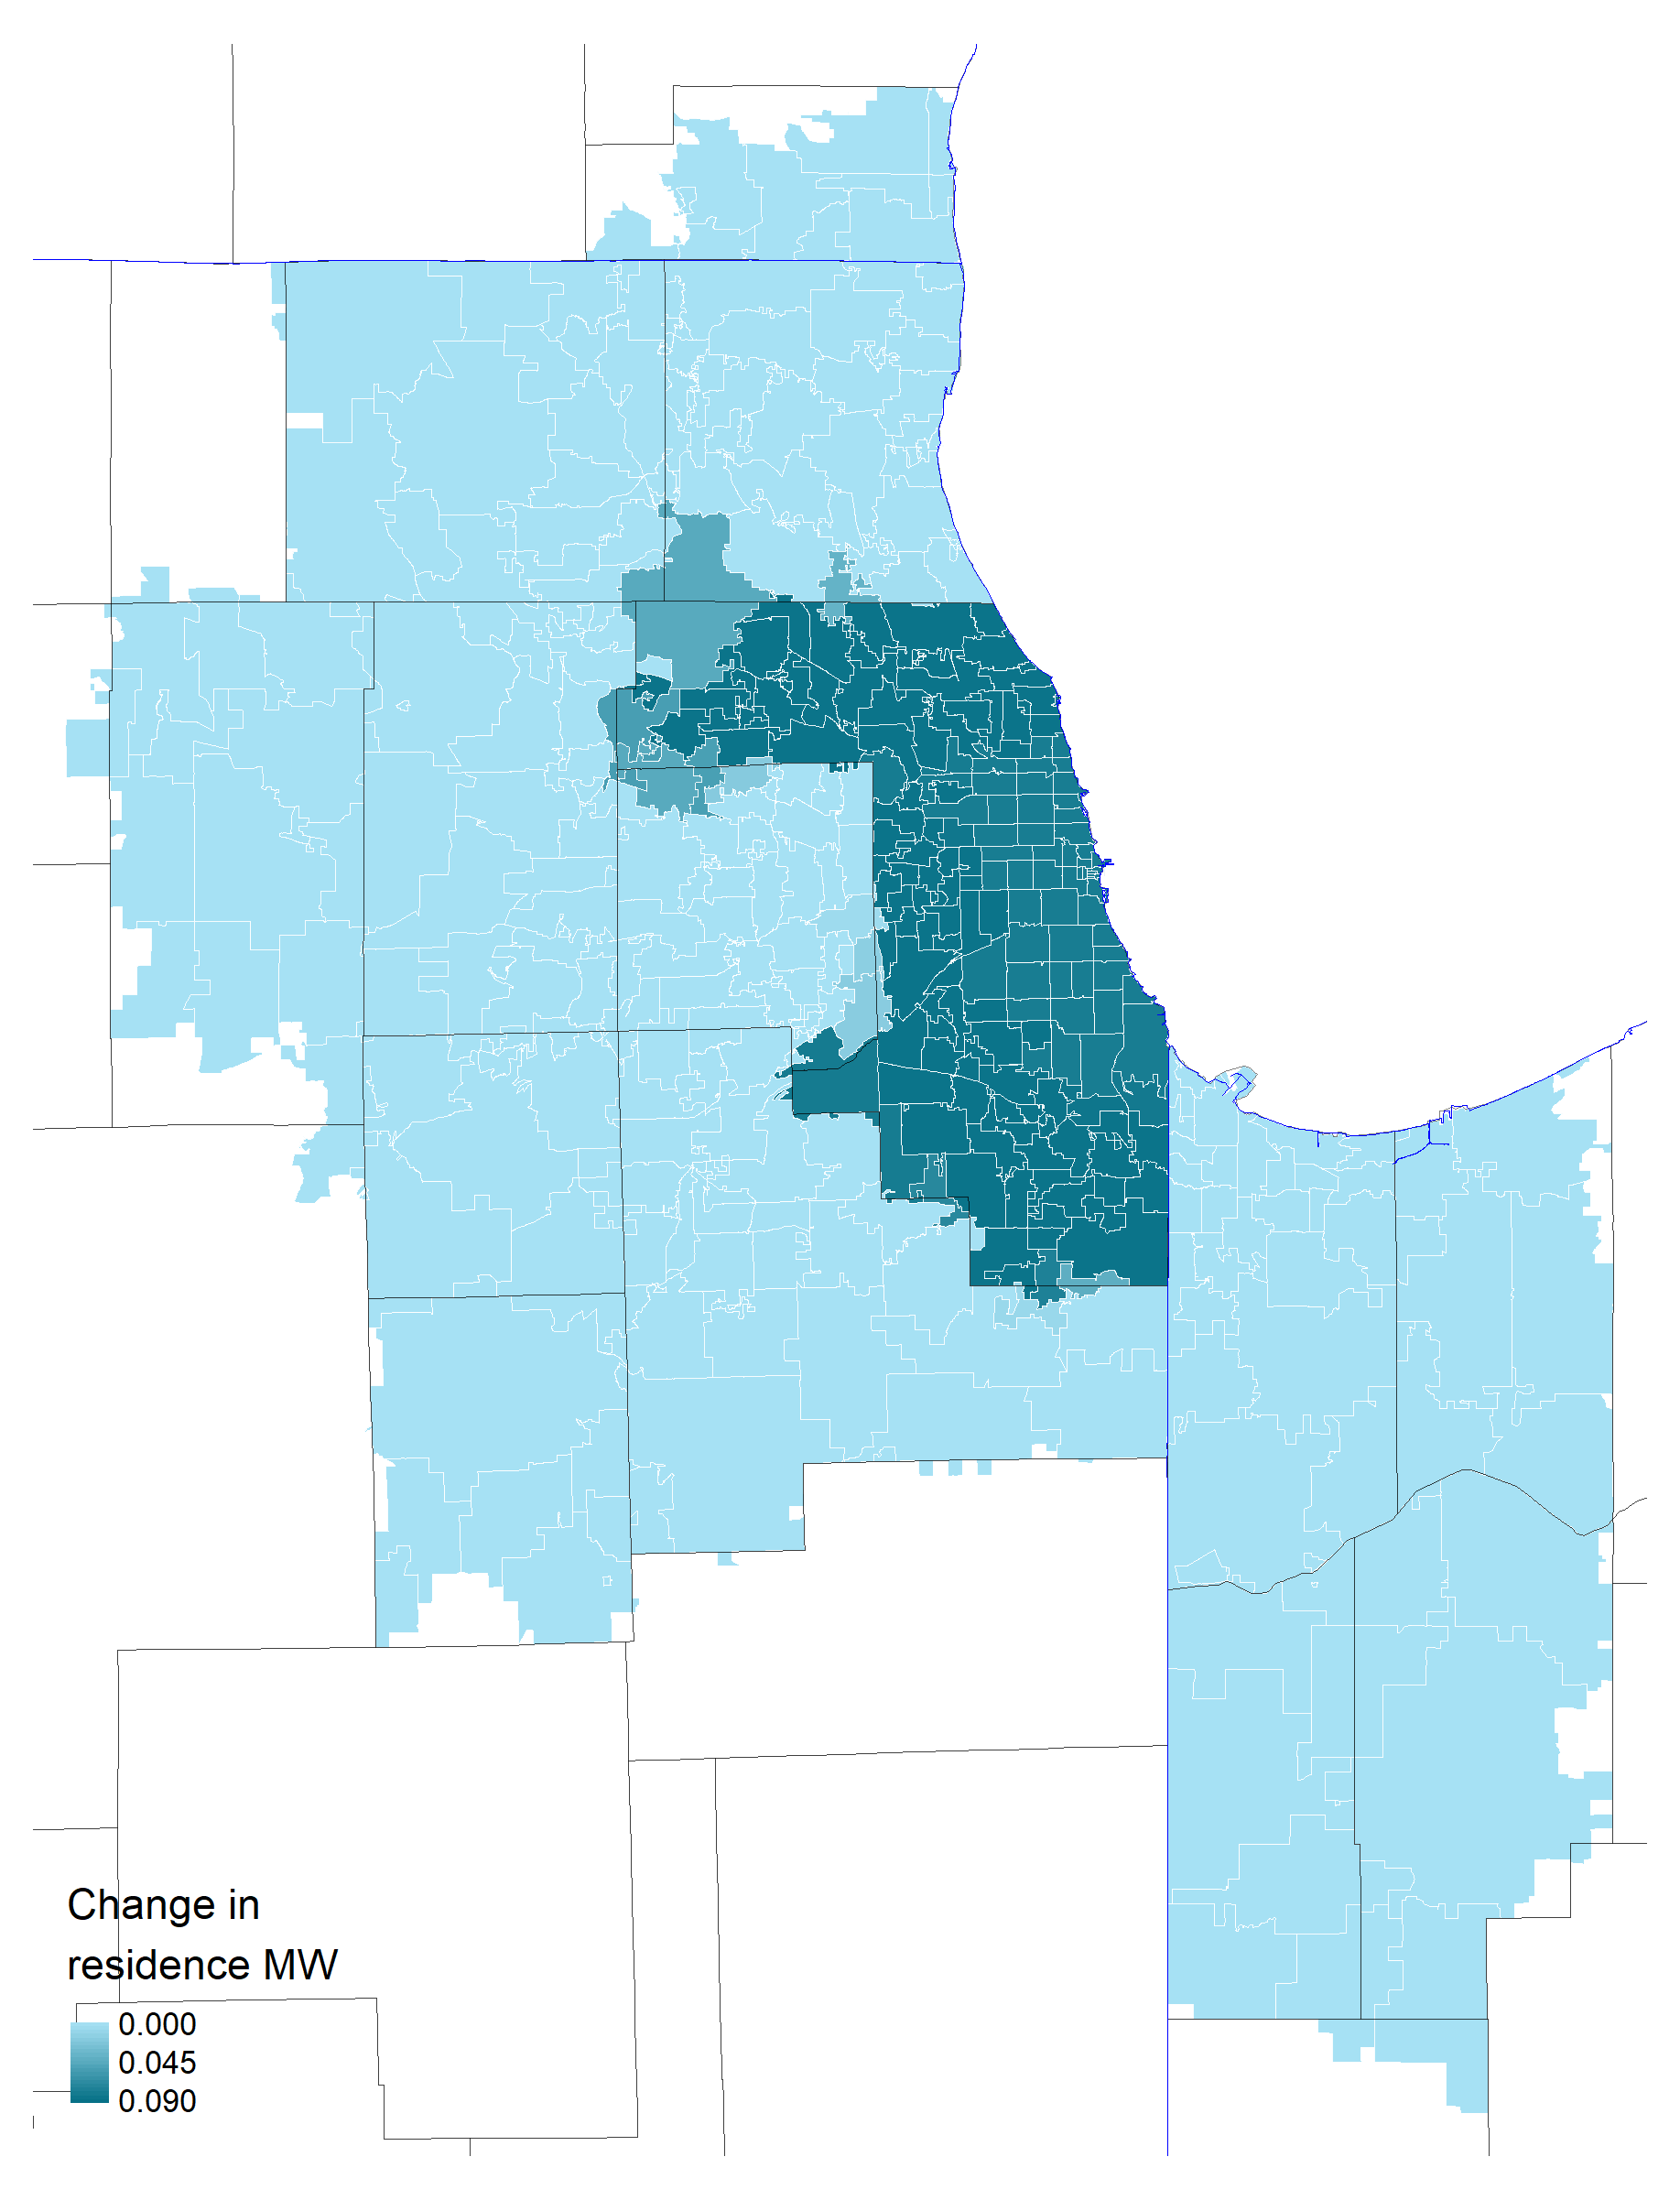
\includegraphics[scale = 0.38]{maps_events/output/chicago_2019-6_statutory_mw.png}
            \end{figure}   
        \end{column}
        \begin{column}{0.56\textwidth}
            Cook County, IL
            \begin{itemize}
                \item Raised local MW from \$12 to \$13 in July 2019. 
                \item State MW is \$8.25 since 2010, and federal MW is \$7.25 since 2009.
                \vspace{2mm}
                \pause
                \item A model where only same-location MW affects rents 
                would miss likely rents increases outside of Cook County
            \end{itemize}
        \end{column}
    \end{columns}
\end{frame}

\begin{frame}
\frametitle{A novel model-based measure of exposure to minimum wages}

    For ZIP code $i$ and month $t$ we define the {\color{red} workplace MW} as
    $$
    {\color{red} \mw^{\wkp}_{it}} = 
    \sum_{z \in \Z(i)} \pi_{i z} \ln \MW_{zt} \ ,
    $$
    %% IMPORTANT: We average the log of the MW! (Not log the average)
    \vspace{-2.5mm}
    where
    \vspace{1mm}
    \begin{itemize} \small
        \item $\MW_{zt}$ is statutory MW in $z$ at time $t$
        \item $\Z(i)$ are workplace locations of $i$'s residents
        \item $\pi_{i z} = L_{i z}/L_i$ is the share of $i$'s residents who work 
        in $z$
    \end{itemize}

    \vspace{3mm}
    The {\color{blue} residence MW} is simply
    $$
    {\color{blue} \mw^{\res}_{it}} = \ln \MW_{it}
    $$
\end{frame}

\begin{frame}[label = chi_example]
\frametitle{A motivating example (continuation)}
    \vspace{-6mm}
    \begin{columns}
        \begin{column}{0.50\textwidth}
            \vspace{-4mm}
            \begin{figure}
                \centering
                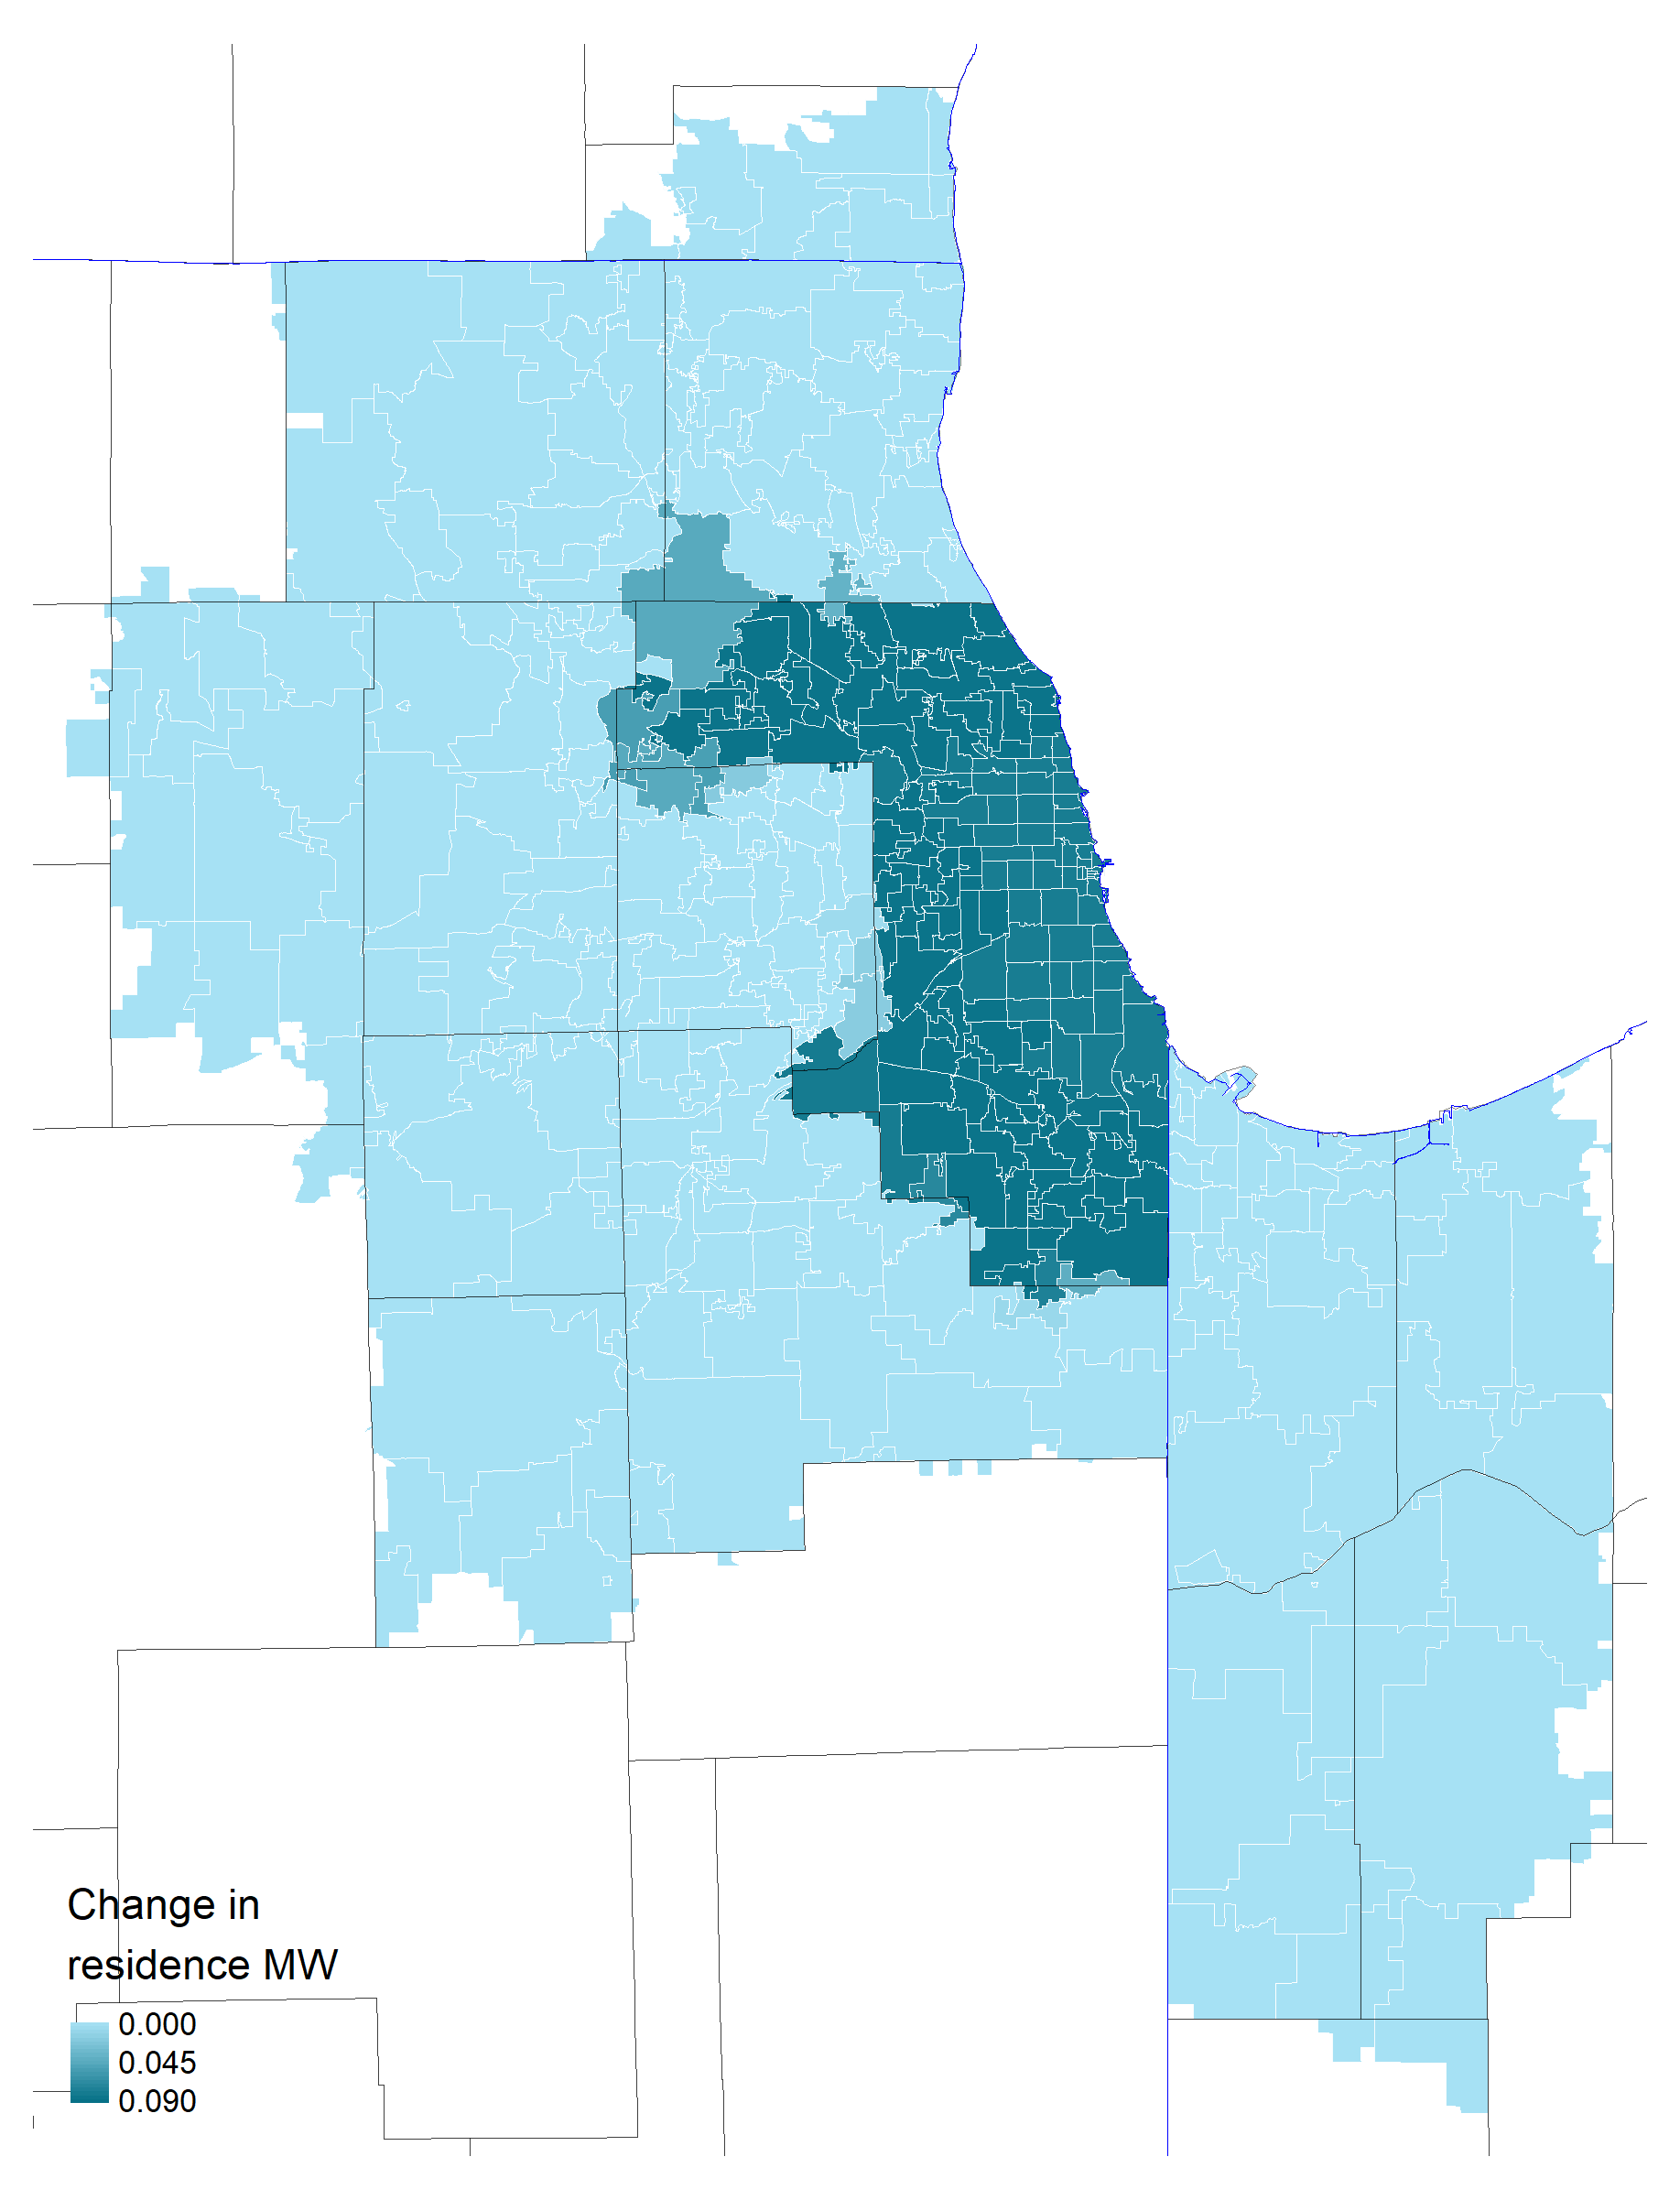
\includegraphics[scale = 0.35]{maps_events/output/chicago_2019-6_statutory_mw.png}
            \end{figure}   
        \end{column}
        \begin{column}{0.50\textwidth}
            \vspace{-4mm}
            \begin{figure}
                \centering
                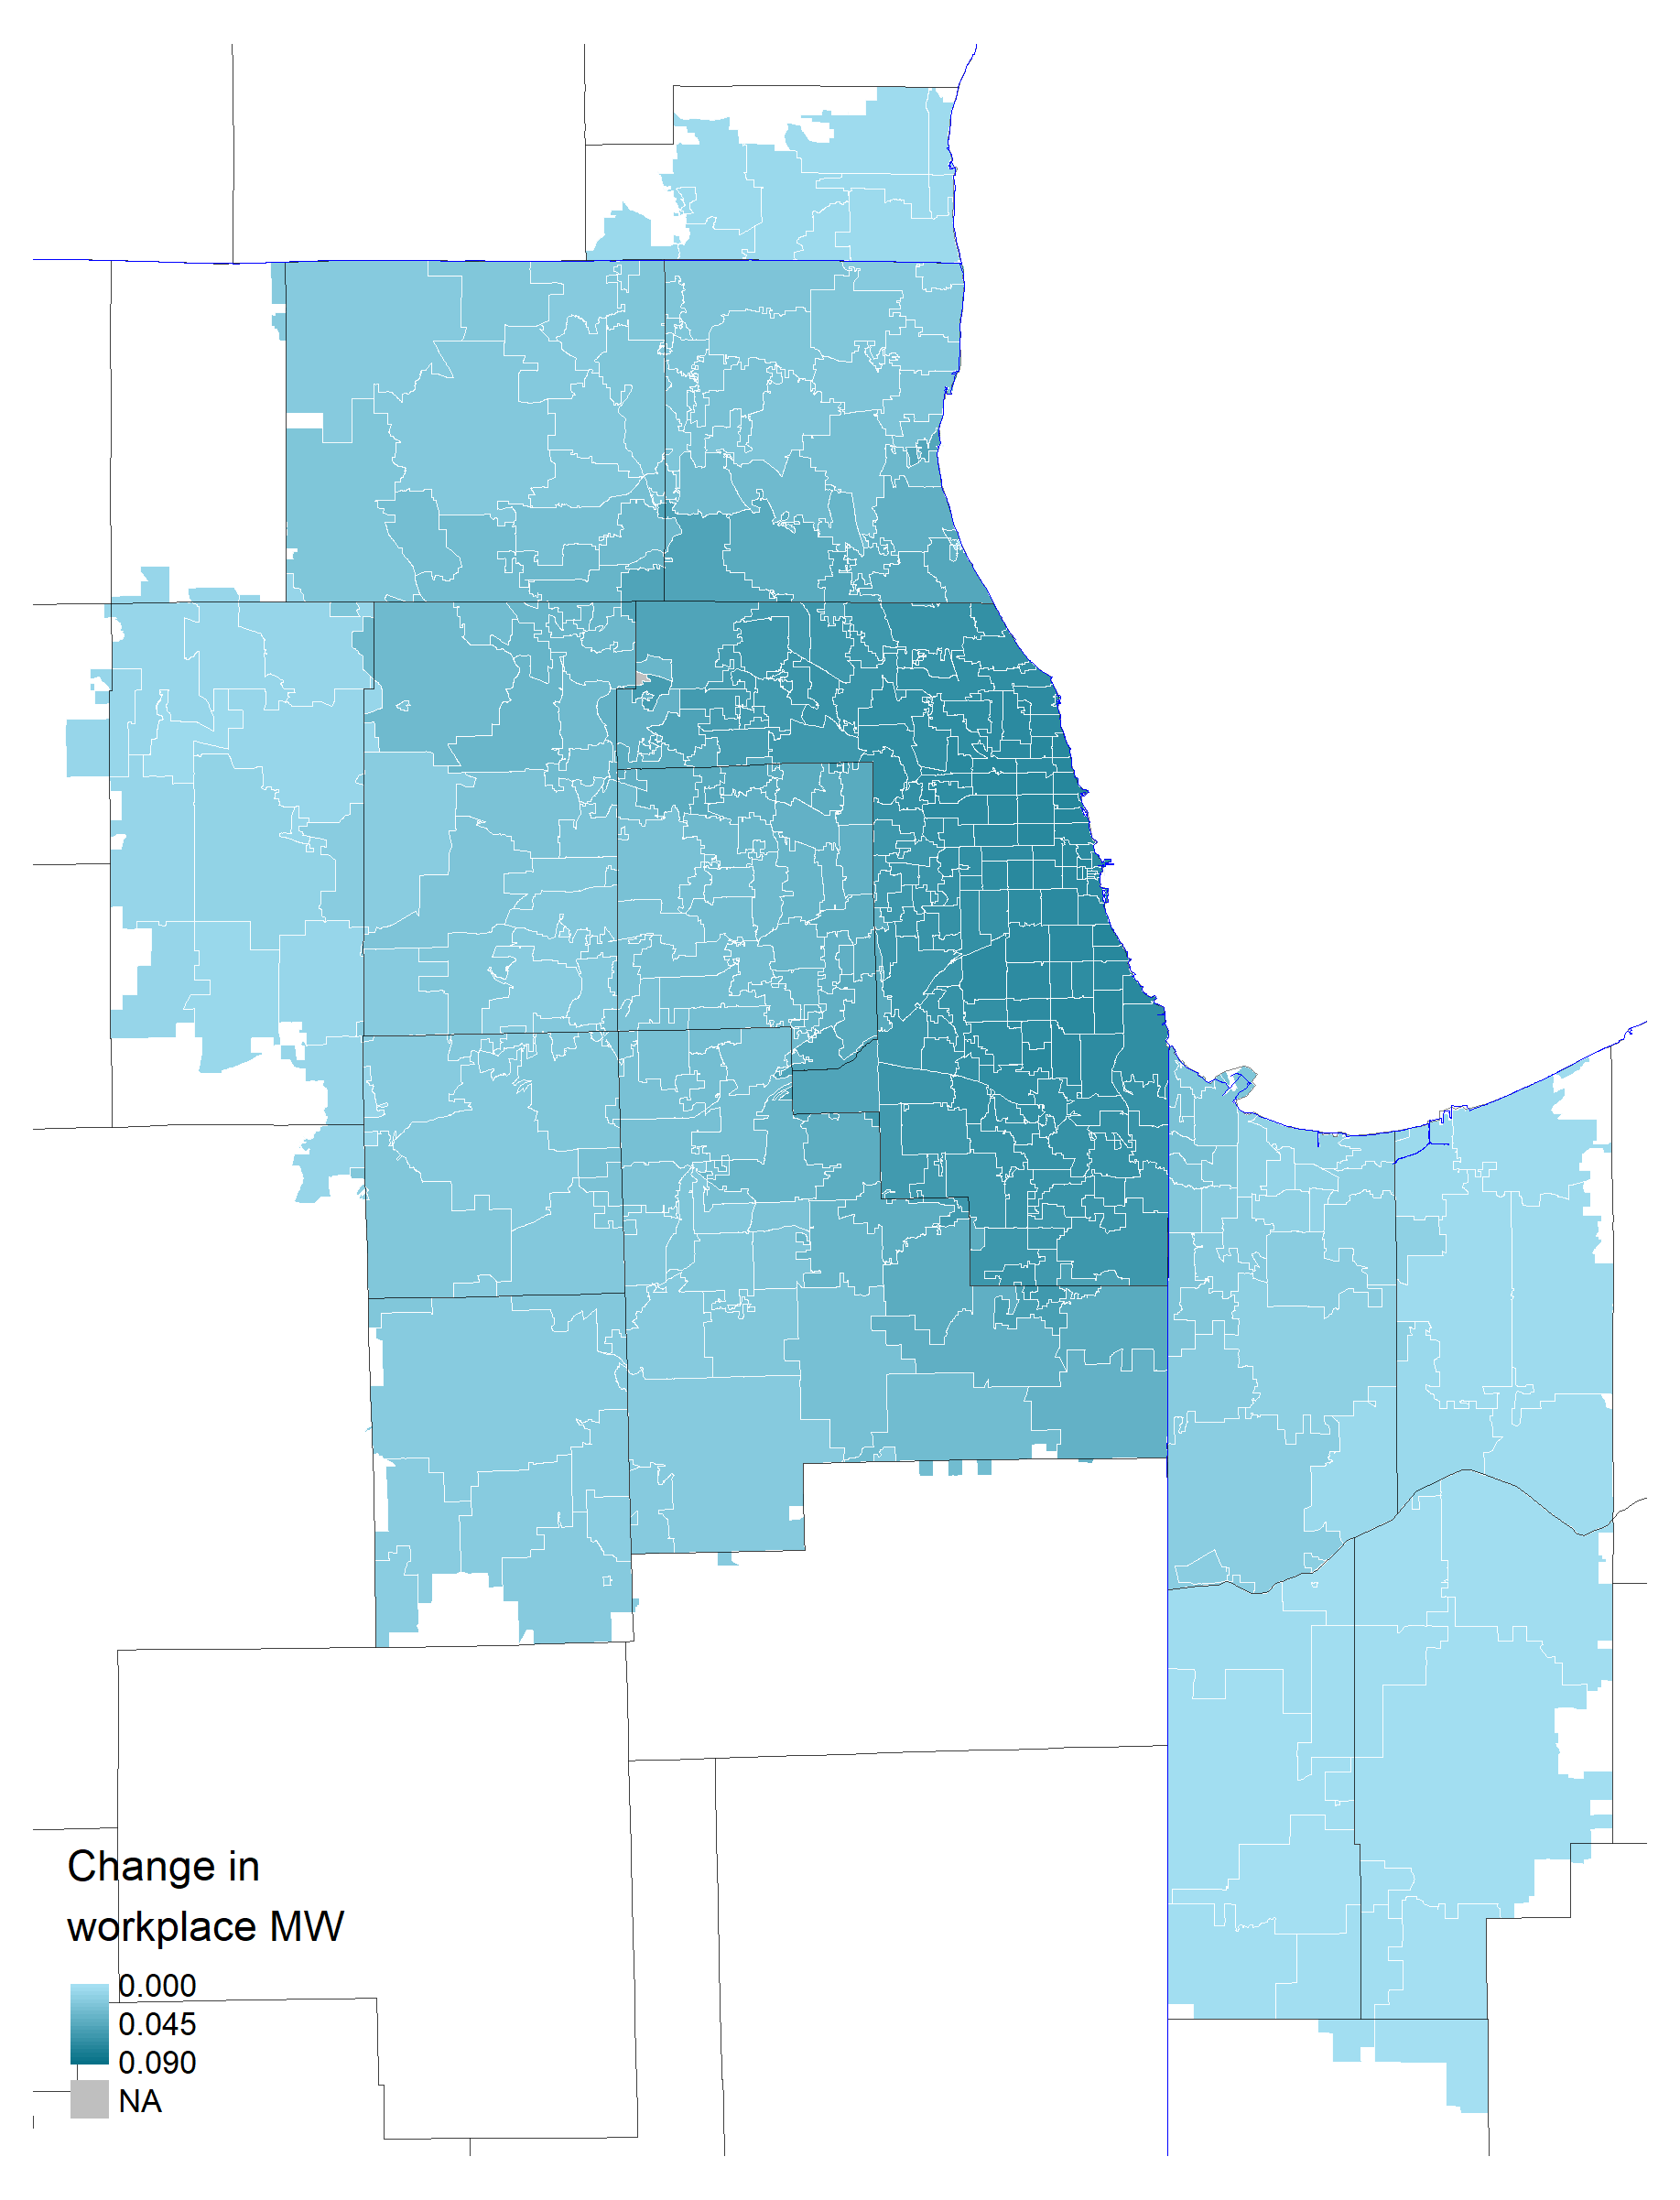
\includegraphics[scale = 0.35]{maps_events/output/chicago2019-6_wkp_mw.png}
            \end{figure}   
        \end{column}
    \end{columns}
    \vspace{3mm}
    \hyperlink{nyc_example}{\beamerbutton{NYC}} 
    \hyperlink{bay_example}{\beamerbutton{Bay Area}}
    \hyperlink{san_diego_example}{\beamerbutton{San Diego}}
    \hyperlink{kc_example}{\beamerbutton{Kansas City}}
\end{frame}

\begin{frame}
    \frametitle{Preview of findings}
    
    Main estimation results
    \begin{itemize}
        \vspace{1mm}
        \item 10 percent $\uparrow$ in {\color{red} workplace MW}
        $\implies$ 0.55 percent $\uparrow$ in rents
        \vspace{1mm}
        \item 10 percent $\uparrow$ in {\color{blue} residence MW}
        $\implies$ 0.21 percent $\downarrow$ in rents
        \vspace{1mm}
        \item 10 percent $\uparrow$ in both measures $\implies$ 0.34 percent $\uparrow$ in rents
    \end{itemize}
    %% Similar magnitude to estimates of MW effects on prices
    
    \vspace{5mm}
    \pause
    Counterfactual increase in federal MW from \$7.25 to \$9 in highly affected areas
    \begin{itemize}
        \vspace{1mm}
        \item Rent changes vary between $-0.4$ to $0.75$ percent (median $0.5$ percent)
        % A rental that costs 2000 would increase to 2100
        \vspace{1mm}
        \item Share pocketed by landlords is between $-15$ and $17$ cents (median $10$ cents)
    \end{itemize}
    %% Distribution are left skewed or negatively skewed
\end{frame}

\begin{frame}
    \frametitle{Outline for Today}
    \tableofcontents[hideallsubsections]
\end{frame}

%%%%%%%%%%%%%%%%%%%%%%%%%%%%%%%%%%%%%%%%%%%%%%%%%%%%%%%%%%%%%%%%%%%%%%%%%%%%%%%%
\section{Partial Equilibrium Model (intuition)}

\begin{frame}
    \frametitle{Overview}
    
    Goals of the model
    \begin{itemize}
        \item Stylized answer to what is the effect of MW changes on rents
        \item Motivate and derive a new measure of exposure to MW
    \end{itemize}
    
    \pause
    \vspace{3mm}
    Assumptions
    \begin{itemize}
        \item A higher MW increases income, which \textit{increases} housing demand
        \item A higher MW increases non-tradable, which \textit{decreases} housing demand
        \item Static model, so residence and workplace locations of workers are fixed
    \end{itemize}
    These assumptions are consistent with the literature

\end{frame}

\begin{frame}
    \frametitle{Comparative statics}
    
    \begin{columns}
        \begin{column}{0.35\textwidth}
            \begin{enumerate}
                \item Equilibrium in ZIP code $i$
                \item \onslide<2->{\color{red} MW increases in some $z$}
                \item \onslide<3->{\color{blue} MW increases in $i$}
            \end{enumerate}
        \end{column}
        \begin{column}{0.65\textwidth}
            \vspace{-2mm}
            \begin{figure}

                \begin{tikzpicture}[scale=.95]
                
                % Axis
                \draw[->, thick] (0,0) -- (6.5,0);
                \draw[->, thick] (0,0) -- (0,6.2);
                \node[left] at (0.2,6.5) {Rents};
                \node[right] at (5,-0.5) {Square feet};
                
                % Base demand and Supply Curves
                \draw (0.3,4.5) -- (4.8,0.5);
                \draw plot [smooth, tension = 1] coordinates {(0.3,1.4) (3,2.8) (5,4.7)};
                       
                \node[right] at (4.8,0.5) {$H_i\left(R_i, P_i^0, \{Y_z^0\}\right)$};
                \node[right] at (5,4.7) {$S_i\left(R_i\right)$};
                
                % Base Eq
                \def\x{2.51}
                \def\y{2.5}
                \draw[dashed] (\x,0) -- (\x,\y);
                \draw[dashed] (0,\y) -- (\x,\y);
                \node[below] at (\x,0) {$H_0^*$};
                \node[left] at (0,\y) {$R_0^*$};
                
                % Equilibrium 1 - Wkp MW increases
                \def\xOne{3.53}
                \def\yOne{3.22}
                \only<2>{
                \draw[color = red] (0.3,6.1) -- (4.8,2.1);
                \node[right] at (4.8,2.1) {$H_i\left(R_i, P_i^0, {\color{red}\{Y_z^1\}}\right)$};

                \draw[dashed, color = red] (\xOne,0) -- (\xOne,\yOne);
                \draw[dashed, color = red] (0,\yOne) -- (\xOne,\yOne);
                \node[below, color = red] at (\xOne,0) {$H_1^*$};
                \node[left, color = red] at (0, \yOne) {$R_1^*$};
                }

                % Equilibrium 1 - Res MW increases
                \def\xTwo{3.07}
                \def\yTwo{2.85}
                \only<3>{
                \draw[dashed, color = red] (0.3,6.1) -- (4.8,2.1);
                \draw[color = blue] (0.3,5.3) -- (4.8,1.3);
                \node[right] at (4.8,1.3) {$H_i\left(R_i, {\color{blue}P_i^2}, {\color{blue}\{Y_z^2\}}\right)$};

                \draw[dashed, color = red] (\xOne,0) -- (\xOne,\yOne);
                \draw[dashed, color = red] (0,\yOne) -- (\xOne,\yOne);
                \node[below, color = red] at (\xOne+.3,0) {$H_1^*$};
                \node[left, color = red] at (0, \yOne+.4) {$R_1^*$};

                \draw[dashed, color = blue] (\xTwo,0) -- (\xTwo,\yTwo);
                \draw[dashed, color = blue] (0,\yTwo) -- (\xTwo,\yTwo);
                \node[below, color = blue] at (\xTwo,0) {$H_2^*$};
                \node[left, color = blue] at (0,\yTwo+.2) {$R_2^*$};
                }
                
                \end{tikzpicture}
                
            \end{figure}
        \end{column}
    \end{columns}

\end{frame}

\begin{frame}
    \frametitle{Representation}

    In this model, assuming homogeneity across workplace locations of
    \begin{enumerate}
        \item elasticity of per-person housing demand to income, and
        \item elasticity of income to the MW
    \end{enumerate}
    we obtain
    \[
    \begin{split}
        \Delta \text{log rents} & = \beta_i  \times \Delta {\color{red}  \text{workplace MW}} \\
                                & + \gamma_i \times \Delta {\color{blue} \text{residence MW}} \\
    \end{split}
    \]

    \vspace{3mm}
    \pause
    Discussion:
    \begin{itemize}
        \item Assumption (1) would hold for homothetic preferences
        \item In estimation can allow for heterogeneity as long as not correlated with MW changes
    \end{itemize}

\end{frame}


%%%%%%%%%%%%%%%%%%%%%%%%%%%%%%%%%%%%%%%%%%%%%%%%%%%%%%%%%%%%%%%%%%%%%%%%%%%%%%%%
\section{Data}

\begin{frame}[label = zillow_data]
    \frametitle{Zillow Data}
    
    \begin{itemize}
        \item Leader online real estate and rental platform in the U.S. {\small (more 
        than 110 million homes and 170 million unique monthly users in 2019).}
        
        \vspace{2mm} \item
        Provides \textit{median} rents data at ZIP code, county, and state levels 
        at a monthly frequency for several housing categories.
        
        \pause
        \vspace{2mm} \item
        We use category single-family, condominium, and cooperative houses (SFCC):
        \begin{itemize}
            \item Most populated series in Zillow
            \item We also estimate our models with other housing categories
        \end{itemize}
        
        \vspace{2mm} \item
        Limitation: Zillow sample is not random.        
        \hyperlink{zillow_pop_density}{\beamerbutton{Zillow ZIP Codes and Population Density}}

    \end{itemize}
\end{frame}

\begin{frame}[label=stat_MW]
    \frametitle{The Statutory MW}
    
    \begin{itemize}
        \item
        Collect MW data at state, county and city levels between Jan 2010 and Dec 2019.
        
        \vspace{2mm}
        \item
        Spatial match:
        \begin{itemize}
            \item Assign census blocks to USPS ZIP codes based on blocks' centroids
            \item Add matching of places, counties, and states using census crosswalk
        \end{itemize}
        
        \vspace{2mm}
        \item
        Assign MWs to each block and take maximum between city, county, state, and federal level
        
        \vspace{2mm}
        \item
        Define statutory MW in ZIP code $i$ and month $t$, $\MW_{it}$, as weighted
        average of MWs at block, using housing units as weights.
         
        \hyperlink{dist_mw_changes}{\beamerbutton{Distribution of MW changes}}

    \end{itemize}
    
\end{frame}

\subsection{MW measures}

\begin{frame}
    \frametitle{Using LODES to construct the workplace MW}
    
    \vspace{2mm}
    
    Construct \textbf{origin-destination matrix} at ZIP code level from LODES 2009 to 2018.
    %% Original data comes at the block level
    
    \vspace{2mm}

    We observe:
    \begin{itemize} \small
        \item Number of workers residing in a ZIP code and working in every other ZIP code.
        \item Analogous matrix for number of workers aged less than 29 and earning less than 
        \$1,251.
    \end{itemize}
    
    \vspace{2mm}
    In our baseline specification we use constant commuter shares from 2017.
    \begin{itemize} \small
        \item Results are robust to using other years and groups.
    \end{itemize}

    \pause
    \vspace{5mm}
    Define the MW measures as
    $$
    {\color{red} \mw^{\wkp}_{it}} = \sum_{z \in \Z(i)} \pi_{i z} \ln \MW_{zt}
    \quad\quad\text{and}\quad\quad
    {\color{blue} \mw^{\res}_{it}} = \ln \MW_{it}
    $$
\end{frame}

%%%%%%%%%%%%%%%%%%%%%%%%%%%%%%%%%%%%%%%%%%%%%%%%%%%%%%%%%%%%%%%%%%%%%%%%%%%%%%%%
\section{Empirical Strategy and Results}

\begin{frame}[label = stat_only_model]
    \frametitle{Empirical (Naive) model}
    
    One may estimate the following first differences model:
    
    $$
    \Delta r_{it} = \tilde\delta_t + 
    \tilde\beta {\color{blue} \Delta \MW^{\text{res}}_{it}} + 
    \Delta \mathbf{X}^{'}_{c(i)t} \tilde\eta + 
    \Delta \tilde\varepsilon_{it} ,
    $$
    
    where    
    \begin{itemize} \small
    \item ZIP code $i$, county $c(i)$, month $t$.
    
    \item \vspace{1mm} $r_{it} = \ln R_{it}$: log of rents per square foot.
    
    \item \vspace{1mm} ${\color{blue} \MW^{\text{res}}_{it}} = \ln \MW_{it}$: log of the residence MW.
    
    \item \vspace{1mm} $\tilde\delta_t$: month fixed effects (ZIP code FE $\tilde\alpha_i 
    $ is 
    implicit).
    
    \item \vspace{.5mm} $\mathbf{X}_{c(i)t}$: time-varying controls at the county level.
    \end{itemize}
\end{frame}

\begin{frame}
    \frametitle{Empirical model}
        
    Now add experienced MW:
    $$
    \Delta r_{it} = \delta_t +
        \beta {\color{red}\Delta \MW^{\text{wrk}}_{it}} +
        \gamma {\color{blue} \Delta \MW^{\text{res}}_{it}} + 
        \Delta \mathbf{X}^{'}_{c(i)t} \eta + 
        \Delta \varepsilon_{it} ,
    $$
    
    where 
    \[
    {\color{red} \MW^{\text{wrk}}_{it}} = 
        \sum_{z \in \Z(i)} \pi_{i z} \ln \underline{w}_{zt}
    \] 
    
    is our measure of access to MW in workplace locations derived from the model.


    \pause
    \vspace{2mm}
    For causal effect of $\beta$ we need:
    $$
    E \left[\Delta \varepsilon_{ict} {\color{red} \Delta 
    \MW^{\text{wrk}}_{i\tau}} 
    \big| {\color{blue}\Delta \MW^{\text{res}}_{it}}, \delta_t, \Delta 
    \mathbf{X}_{c(i)t} \right] = 0
    \quad \quad \forall \tau \in \left[ \underline{T}, \overline{T} \right]
    $$
    
    \pause
    \vspace{2mm}
    \textbf{In words}: conditional on FEs, controls, and {\color{blue} MW in same ZIP 
    code}, unobserved innovations to rent shocks are uncorrelated with past and future 
    values of log MW changes {\color{red} in nearby ZIP codes}.
\end{frame}

\begin{frame}
    \frametitle{Discussion Identification Assumption}
    
    Thus, for causal effect of $\beta$ we need:
    $$
    E \left[\Delta \varepsilon_{it} \Delta \MW^{\text{wrk}}_{it}  
    \big| \Delta \MW^{\text{res}}_{it}, \delta_t, \Delta 
    \mathbf{X}_{c(i)t} \right] = 0
    \quad \quad \forall \tau \in \left[ \underline{T}, \overline{T} \right]
    $$
    \vspace{.5mm}
    Analogously, for causal effect of $\gamma$ we need:
    $$
    E \left[\Delta \varepsilon_{it} \Delta \MW^{\text{res}}_{it}  
    \big| \Delta \MW^{\text{wrk}}_{it}, \delta_t, \Delta \mathbf{X}_{c(i)t} 
    \right] = 0
    \quad \quad \forall \tau \in \left[ \underline{T}, \overline{T} \right]
    $$
    
    \pause
    \vspace{.5mm}
    \textbf{Is this plausible?}
    \begin{itemize} \small
        \vspace{.5mm}
        \item MW policies are rarely set by considering differential dynamics of the 
        rental housing market within metropolitan areas.
        %% For example, the Congressional Budget Office (CBO) doesn't mention rents even 
        %% once in it's study of the effects of the Wage Act of 2021
        %% https://www.cbo.gov/system/files/2021-02/56975-Minimum-Wage.pdf
        
        \vspace{.5mm}
        \item Furthermore, there is substantial heterogeneity in the housing market 
        across ZIP codes.
        
        \vspace{.5mm}
        \item Indirectly test assumption through pre-trends, assuming no anticipatory 
        effects in housing market.
    \end{itemize}
\end{frame}


\begin{frame}[label = dyn_model]
    \frametitle{Testing Identification with a Dynamic model}
    
    Adding leads and lags of the experienced log MW:
    
    $$
    \Delta r_{it} = \delta_t
        + \sum_{r=-s}^{s} \beta_r \Delta \MW^{\text{exp}}_{i,t+r}
        + \gamma \Delta \MW^{\text{res}}_{it}
        + \Delta \mathbf{X}^{'}_{c(i)t}\eta
        + \Delta \varepsilon_{it}
    $$    
    where $\{\beta_r\}_{r=-s}^{s}$ are the dynamic coefficients.
    
    \vspace{3mm}

    Analogously, one can add instead the leads and lags of the log residence MW
    to test the identification assumption of $\gamma$.
\end{frame}

%%%%%%%%%%%%%%%%%%%%%%%%%%%%%%%%%%%%%%%%%%%%%%%%%%%%%%%%%%%%%%%%%%%%%%%%%%%%%%%%
\section{Results}

\subsection{Main Results}

\begin{frame}[label = static_tab]
    \frametitle{Static Model}

    %\begin{table}
    \label{tab:static}
    \scalebox{0.8}{
        \begin{tabular}{l*{4}{c}}
            \toprule
            & \multicolumn{1}{c}{\shortstack{Change wkp.\ MW\\$\Delta\mw_{it}^{\wkp}$}}
                & \multicolumn{3}{c}{\shortstack{Change log rents\\$\Delta r_{it}$}} \\ \cmidrule(lr){2-2}\cmidrule(lr){3-5}
                                               & (1)   & (2)   & (3)   & (4)            \\ \midrule
            Change residence MW 
                      $\Delta\mw_{it}^{\res}$  &  #4#  &  #4#  &       &  #4#     \\
                                               & (#4#) & (#4#) &       & (#4#)    \\
            Change workplace MW 
                       $\Delta\mw_{it}^{\wkp}$ &       &       &  #4#  & #4#      \\
                                               &       &       & (#4#) & (#4#)    \\ \midrule
            Sum of coefficients                &       &       &       &  #4#     \\
                                               &       &       &       & (#4#)    \\ \midrule
            County-quarter economic controls   &  Yes  & Yes   & Yes   & Yes      \\
            P-value equality                   &       &       &       & #4#      \\
            R-squared                          &  #4#  &  #4#  &  #4#  & #4#      \\
            Observations                       & #0,#  & #0,#  & #0,#  & #0,#     \\\bottomrule
        \end{tabular}
    }
\end{table}

    \hyperlink{example_pred_chi_07_2019}{\beamerbutton{Example Predictions for Chicago July 2019}}
\end{frame}

\begin{frame}[label = dyn_baseline_plot]
    \frametitle{Including leads and lags of workplace MW}

    \begin{figure}
        \centering
        \vspace{-2mm}
        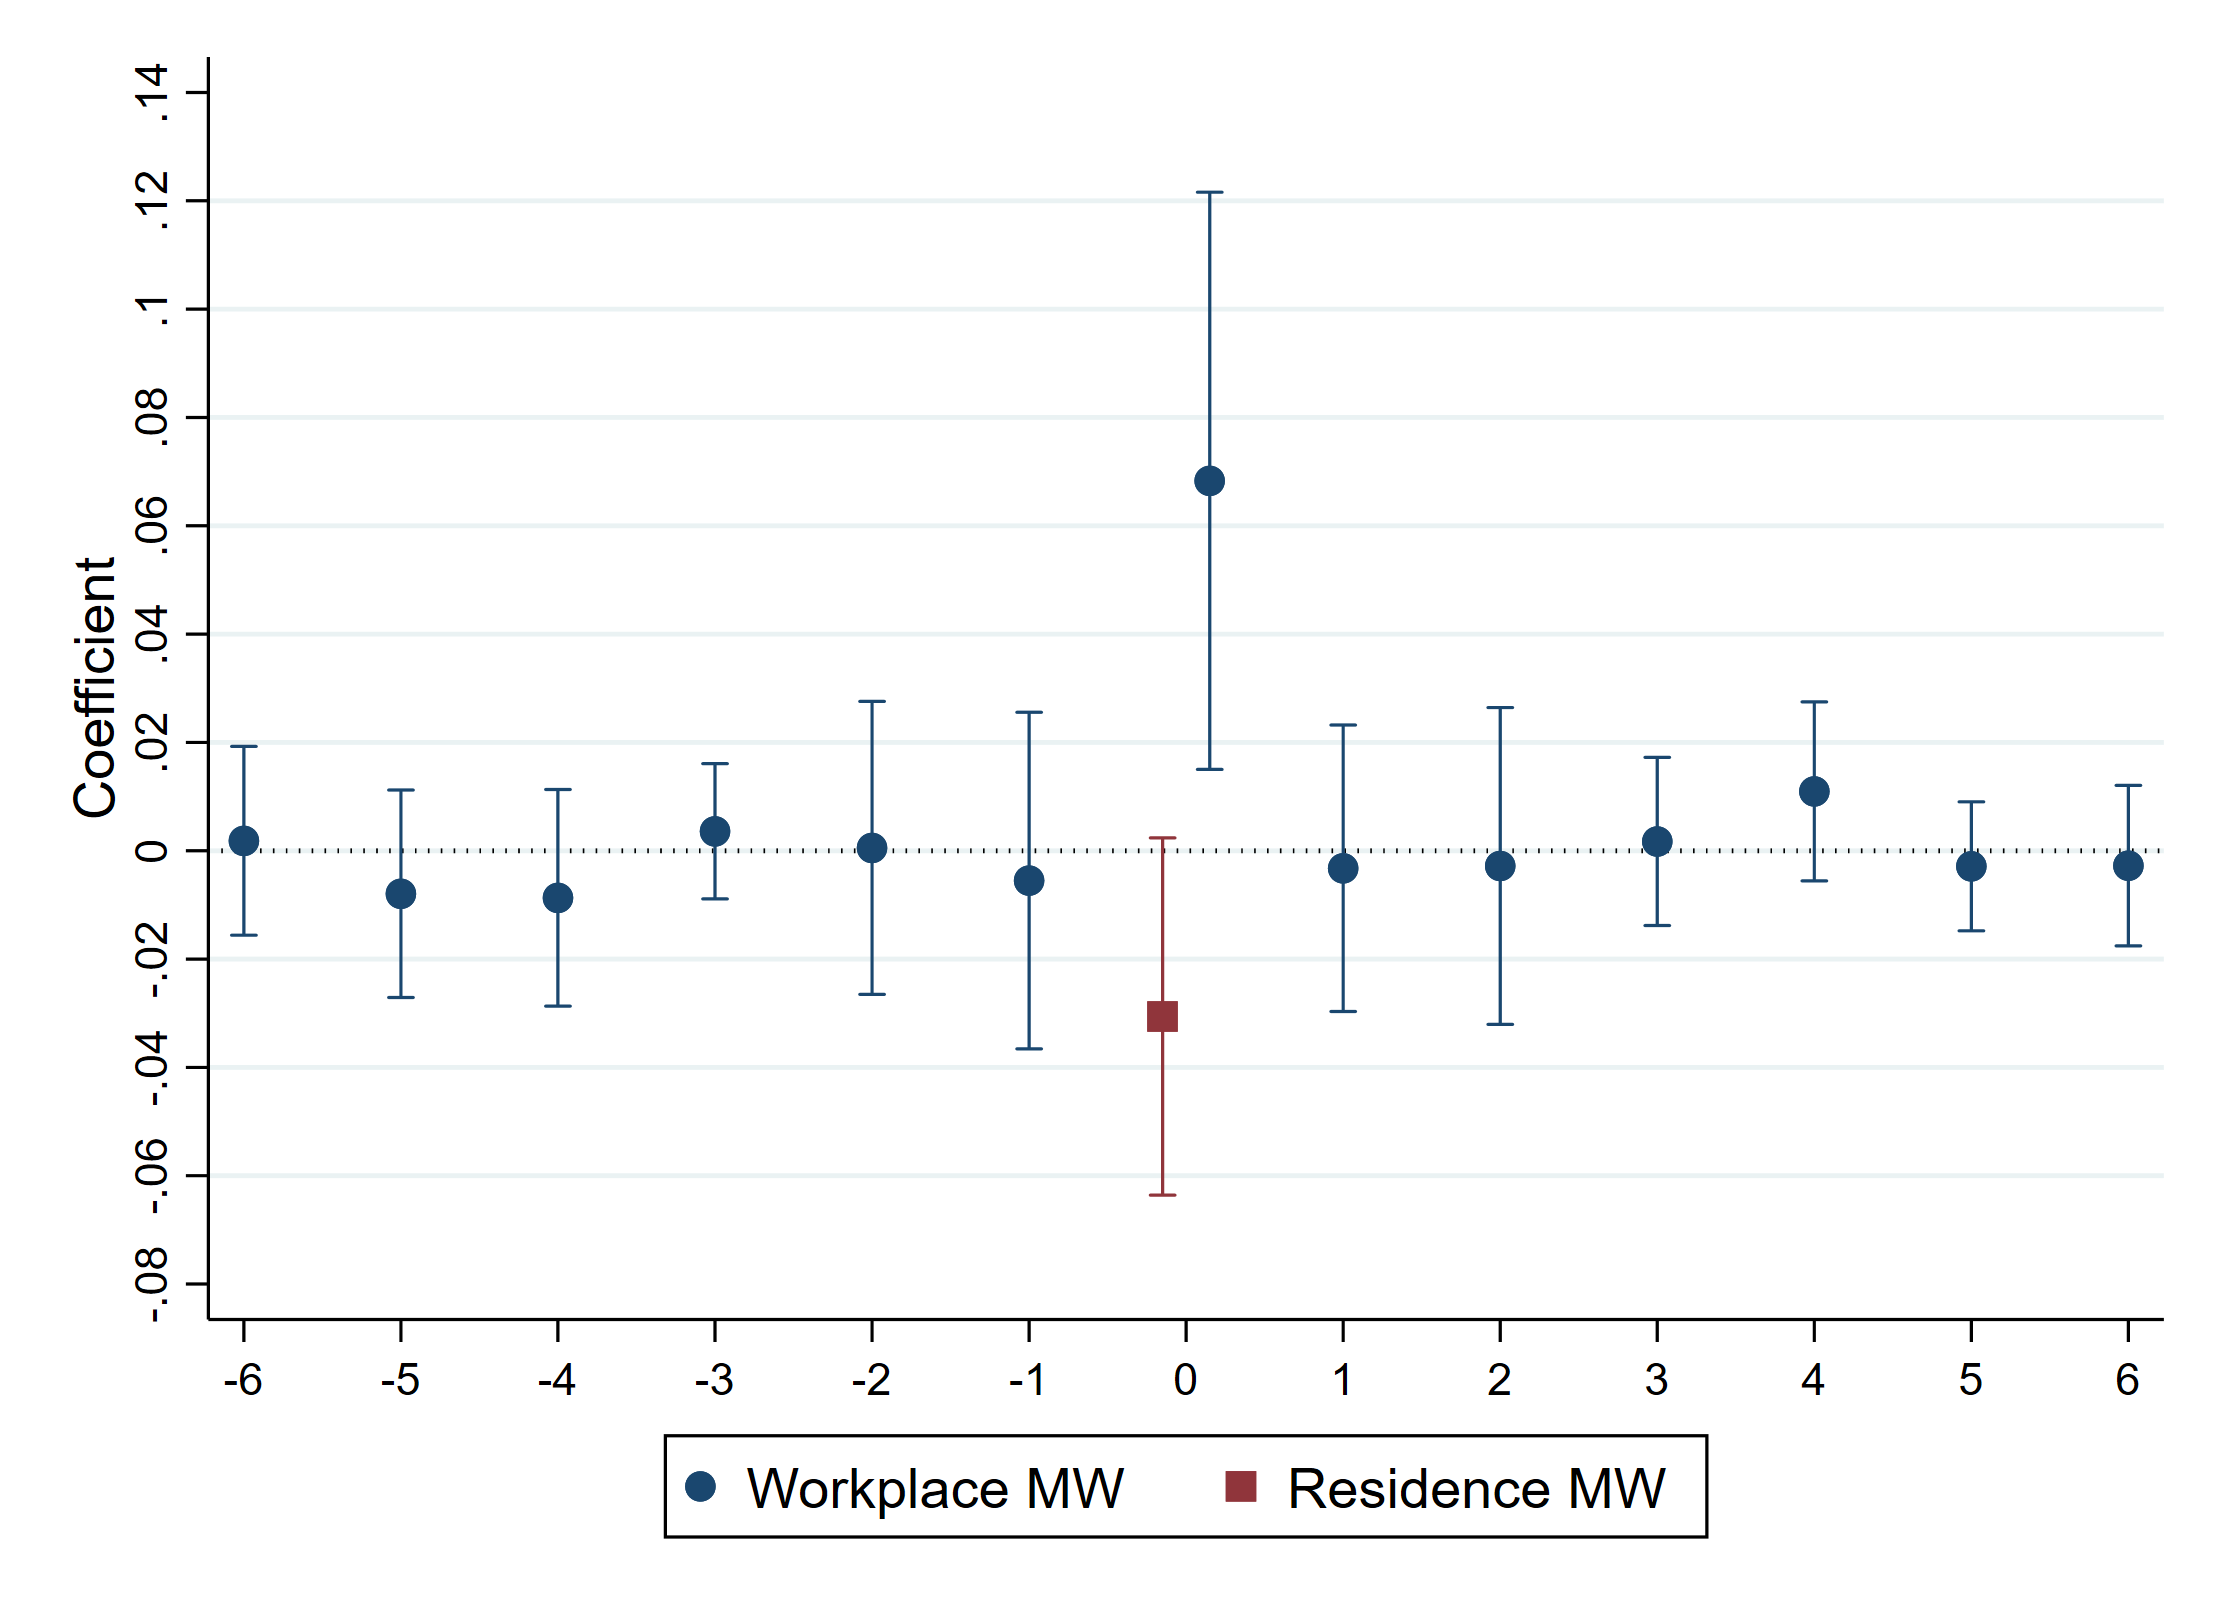
\includegraphics[width=0.70\textwidth]{fd_baseline/output/fd_both_mw_wkp_only_dynamic.png}
    \end{figure}
    
\end{frame}

\begin{frame}[label = robus_sample]
    \frametitle{Robustness checks and Sample Selection}

    Concerns about differential geographic trends across treated
    \begin{itemize}
        \item Inclusion of non-parametric geographical trends
        \item Inclusion of ZIP code-specific parametric trends
        \item Use only MW changes that are not pre-announced (work in progress)
        \item Stack events a lá \cite{CegnizEtAl2019} (work in progress)
    \end{itemize}
    \hyperlink{robustness_geo}{\beamerbutton{Robustness results}}

    \vspace{3mm}
    Concerns that results are particular to our sample or not generalizable
    \begin{itemize}
        \item Estimate model on fully balanced and unbalanced panels
        \item Reweight observations to match characteristics of average urban ZIP code
    \end{itemize}
    \hyperlink{robustness_geo}{\beamerbutton{Sample-issues results}}
    
    \vspace{3mm}
    Concerns about workplace MW definition:
    \begin{itemize}
        \item Estimate under different commuter shares.
    \end{itemize}
    \hyperlink{robustness_exp_mw}{\beamerbutton{Sensitivity to alternative commuter shares}}
\end{frame}

%%%%%%%%%%%%%%%%%%%%%%%%%%%%%%%%%%%%%%%%%%%%%%%%%%%%%%%%%%%%%%%%%%%%%%%%%%%%%%%%
\section{The incidence of a counterfactual federal MW change}

\begin{frame}
    \frametitle{Overview}
    
    Entire commuting structure determines the incidence of MW policies.
    \begin{itemize}
        \vspace{1mm}
        \item In some ZIP codes both residence and workplace MW increase
        \vspace{1mm}
        \item Other nearby ZIP codes are affected only through workplace
    \end{itemize}
    
    \pause
    \vspace{3mm}
    Consider an increase of the federal MW to \$9 in January 2020.
    \begin{itemize}
        \vspace{1mm}
        \item Changes income $\{\Delta Y_i\}_{i\in\Z}$ and housing expenditure $\{\Delta H_i\}_{i\in\Z}$
    \end{itemize}
    
    \pause
    \vspace{3mm}
    How much out of each extra dollar is captured by landlords?
   
\end{frame}

\begin{frame}
    \frametitle{Pass-through coefficients}

    Define pass-through coefficients as    
    \begin{equation*}
        \rho_i := \frac{\Delta H_i}{\Delta Y_i} =  \frac{h^{\text{Post}}_i R^{\text{Post}}_i - h^{\text{Pre}}_i R^{\text{Pre}}_i}{\Delta Y_i}
    \end{equation*}
    where 
    \begin{itemize}
        \item $h$ denotes rented space in $i$ (square feet)
        \item Pre and Post indicate moments before and after the increase
    \end{itemize}

    \pause
    \vspace{3mm}
    Change in rented space are unobserved. We assume $h^{\text{Pre}}_i = h^{\text{Post}}_i = h_i$ so
    \begin{equation*}
        \rho_i = \frac{h^{\text{Post}}_i R^{\text{Post}}_i - h^{\text{Pre}}_i R^{\text{Pre}}_i}{\Delta Y_i} = h_i \frac{\Delta R_i}{\Delta Y_i}
    \end{equation*}
    If $\Delta h_i > 0$ then our estimate of $\rho_i$ is a lower bound.

\end{frame}

\begin{frame}
    \frametitle{Pass-through under the model}

    According to the model,
    $$
    \Delta \ln R_i = \beta \MW_i^{\text{wkr}} + \gamma \MW_i^{\text{res}}
    $$
    We also define
    $$
    \Delta \ln Y_i = \varepsilon \MW_i^{\text{wkr}}
    $$

    \pause
    \vspace{2mm}
    Algebra implies
    \begin{equation*}
        \begin{split}
            \rho_i & = h_i \left[ 
                \frac{\exp \left(\Delta \ln R_i + \ln R_i \right) - R_i }{\exp \left( \Delta \ln Y_i + \ln Y_i \right) - Y_i }
                \right] \\
                & = \alpha_i \left[
                    \frac{\exp \left( \beta \MW_i^{\text{wkr}} + \gamma \MW_i^{\text{res}} \right) - 1 }{\exp \left( \varepsilon \MW_i^{\text{wkr}} \right) - 1 }
                \right]
        \end{split}
    \end{equation*}
    where
    \begin{itemize}
        \item $\alpha_i = \frac{h_i R_i}{Y_i}$ is the share of $i$'s expenditure in housing
    \end{itemize}

    \vspace{2mm}
    We use our estimates to compute $\rho_i$ for urban ZIP codes.
    %% URBAN ZIP codes according to who? KNOW THIS
\end{frame}

\begin{frame}
    \frametitle{Increases in residence and workplace MWs}
    \begin{figure}
        \begin{subfigure}{0.51\textwidth}
            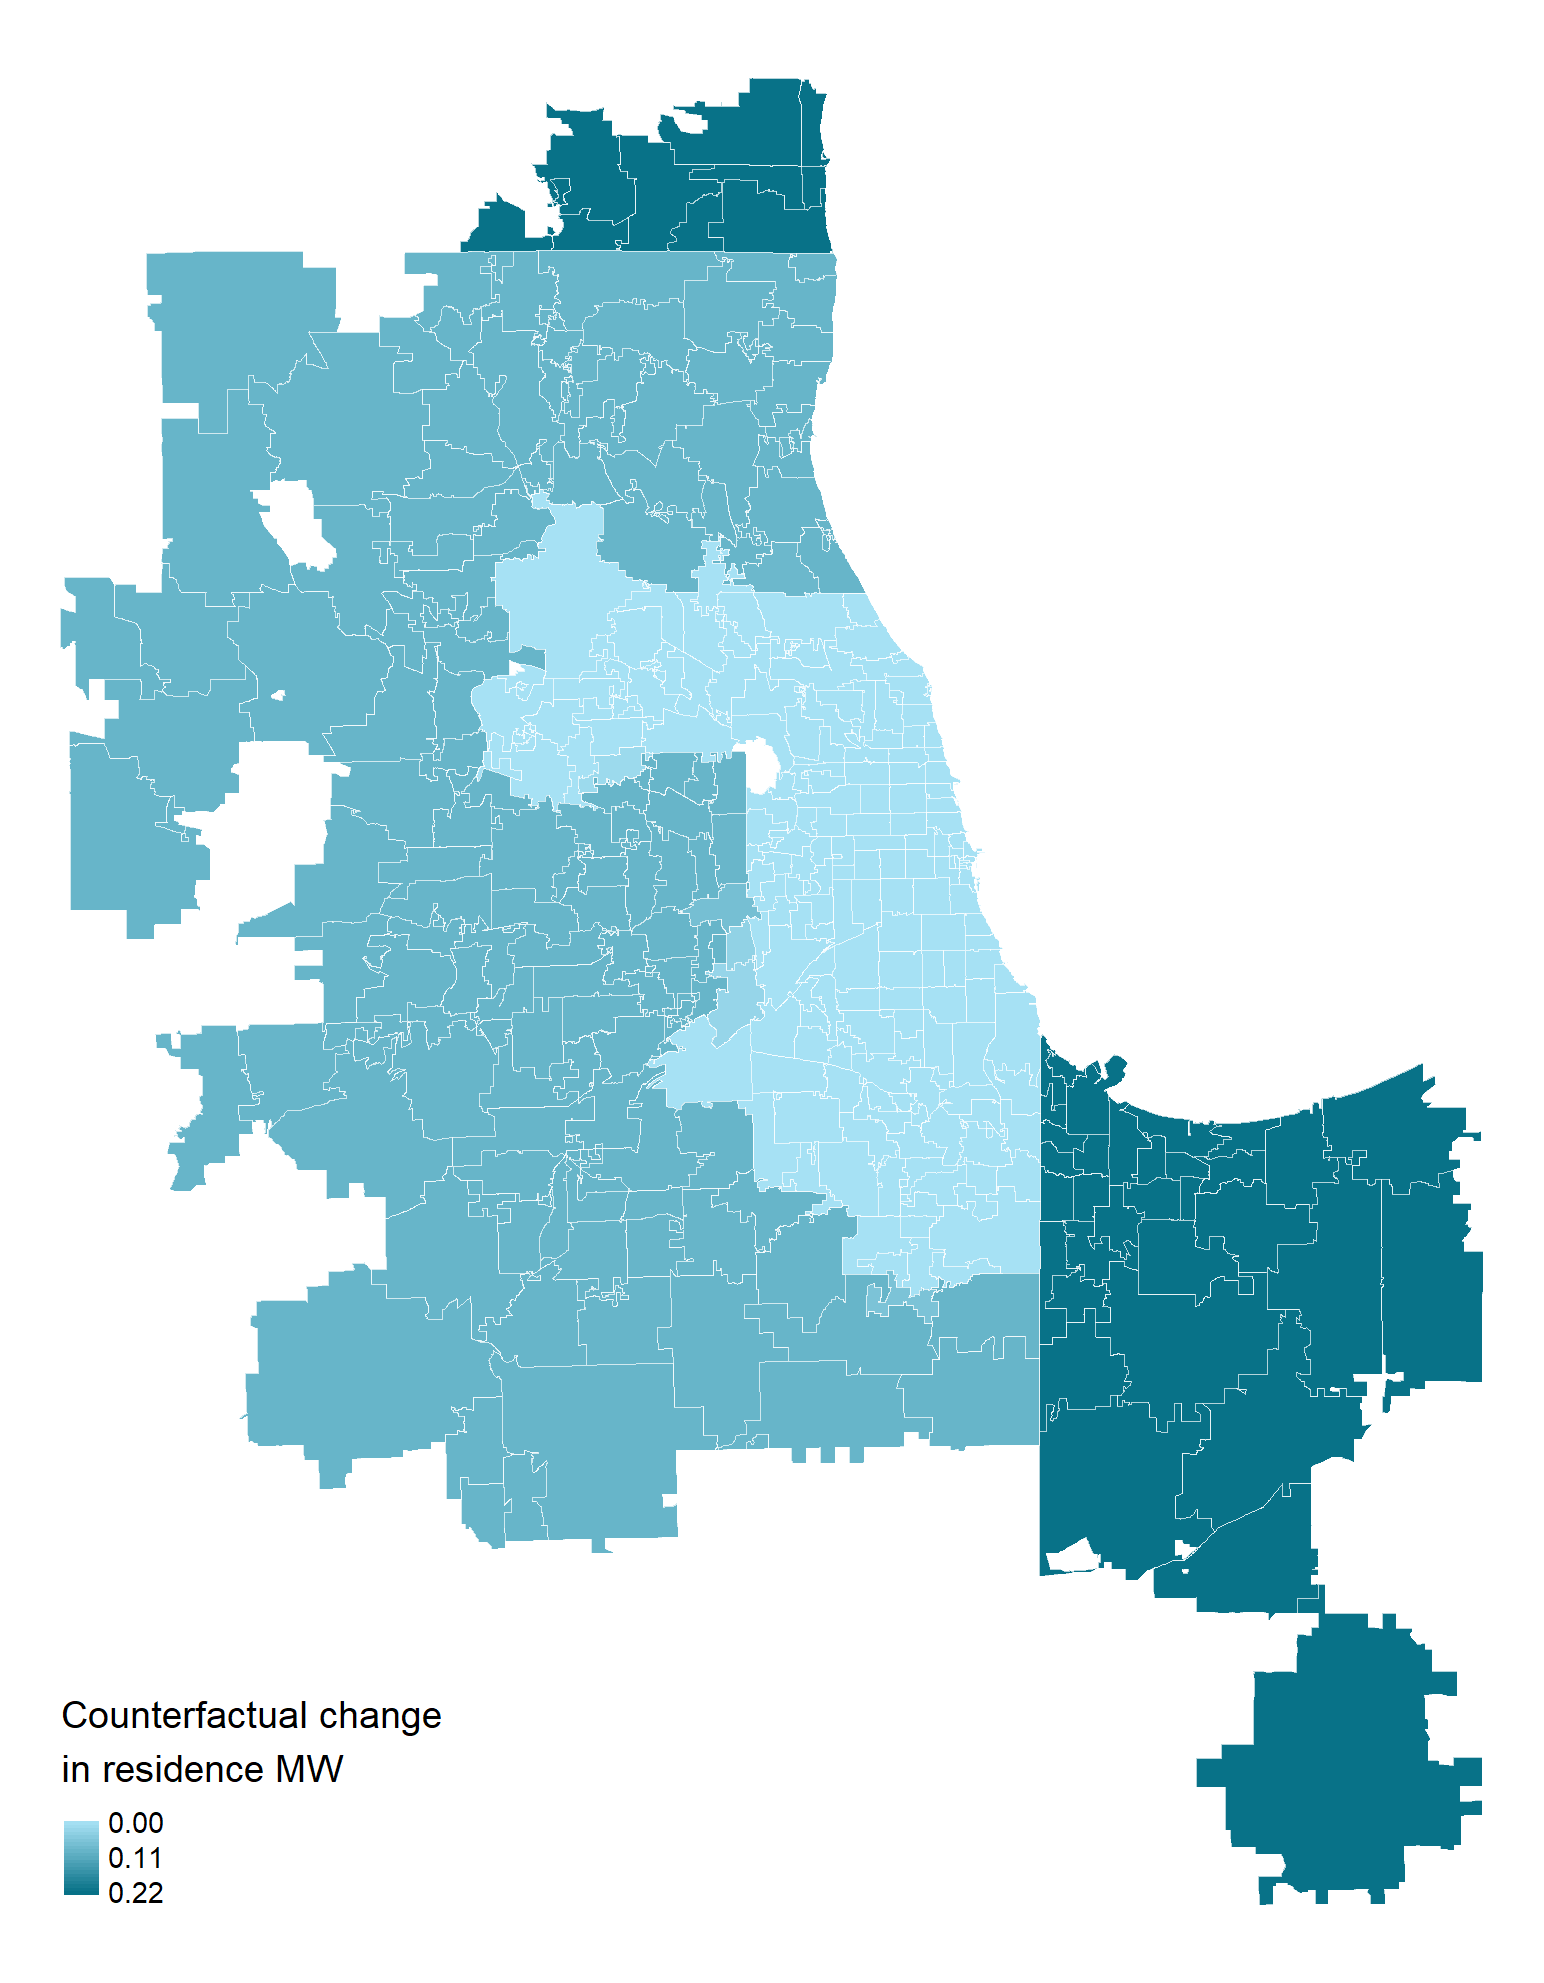
\includegraphics[width = 0.99\textwidth]{counterfactuals/output/chicago_d_mw_res.png}
            \caption*{Residence MW}
        \end{subfigure}%
        \begin{subfigure}{0.51\textwidth}
            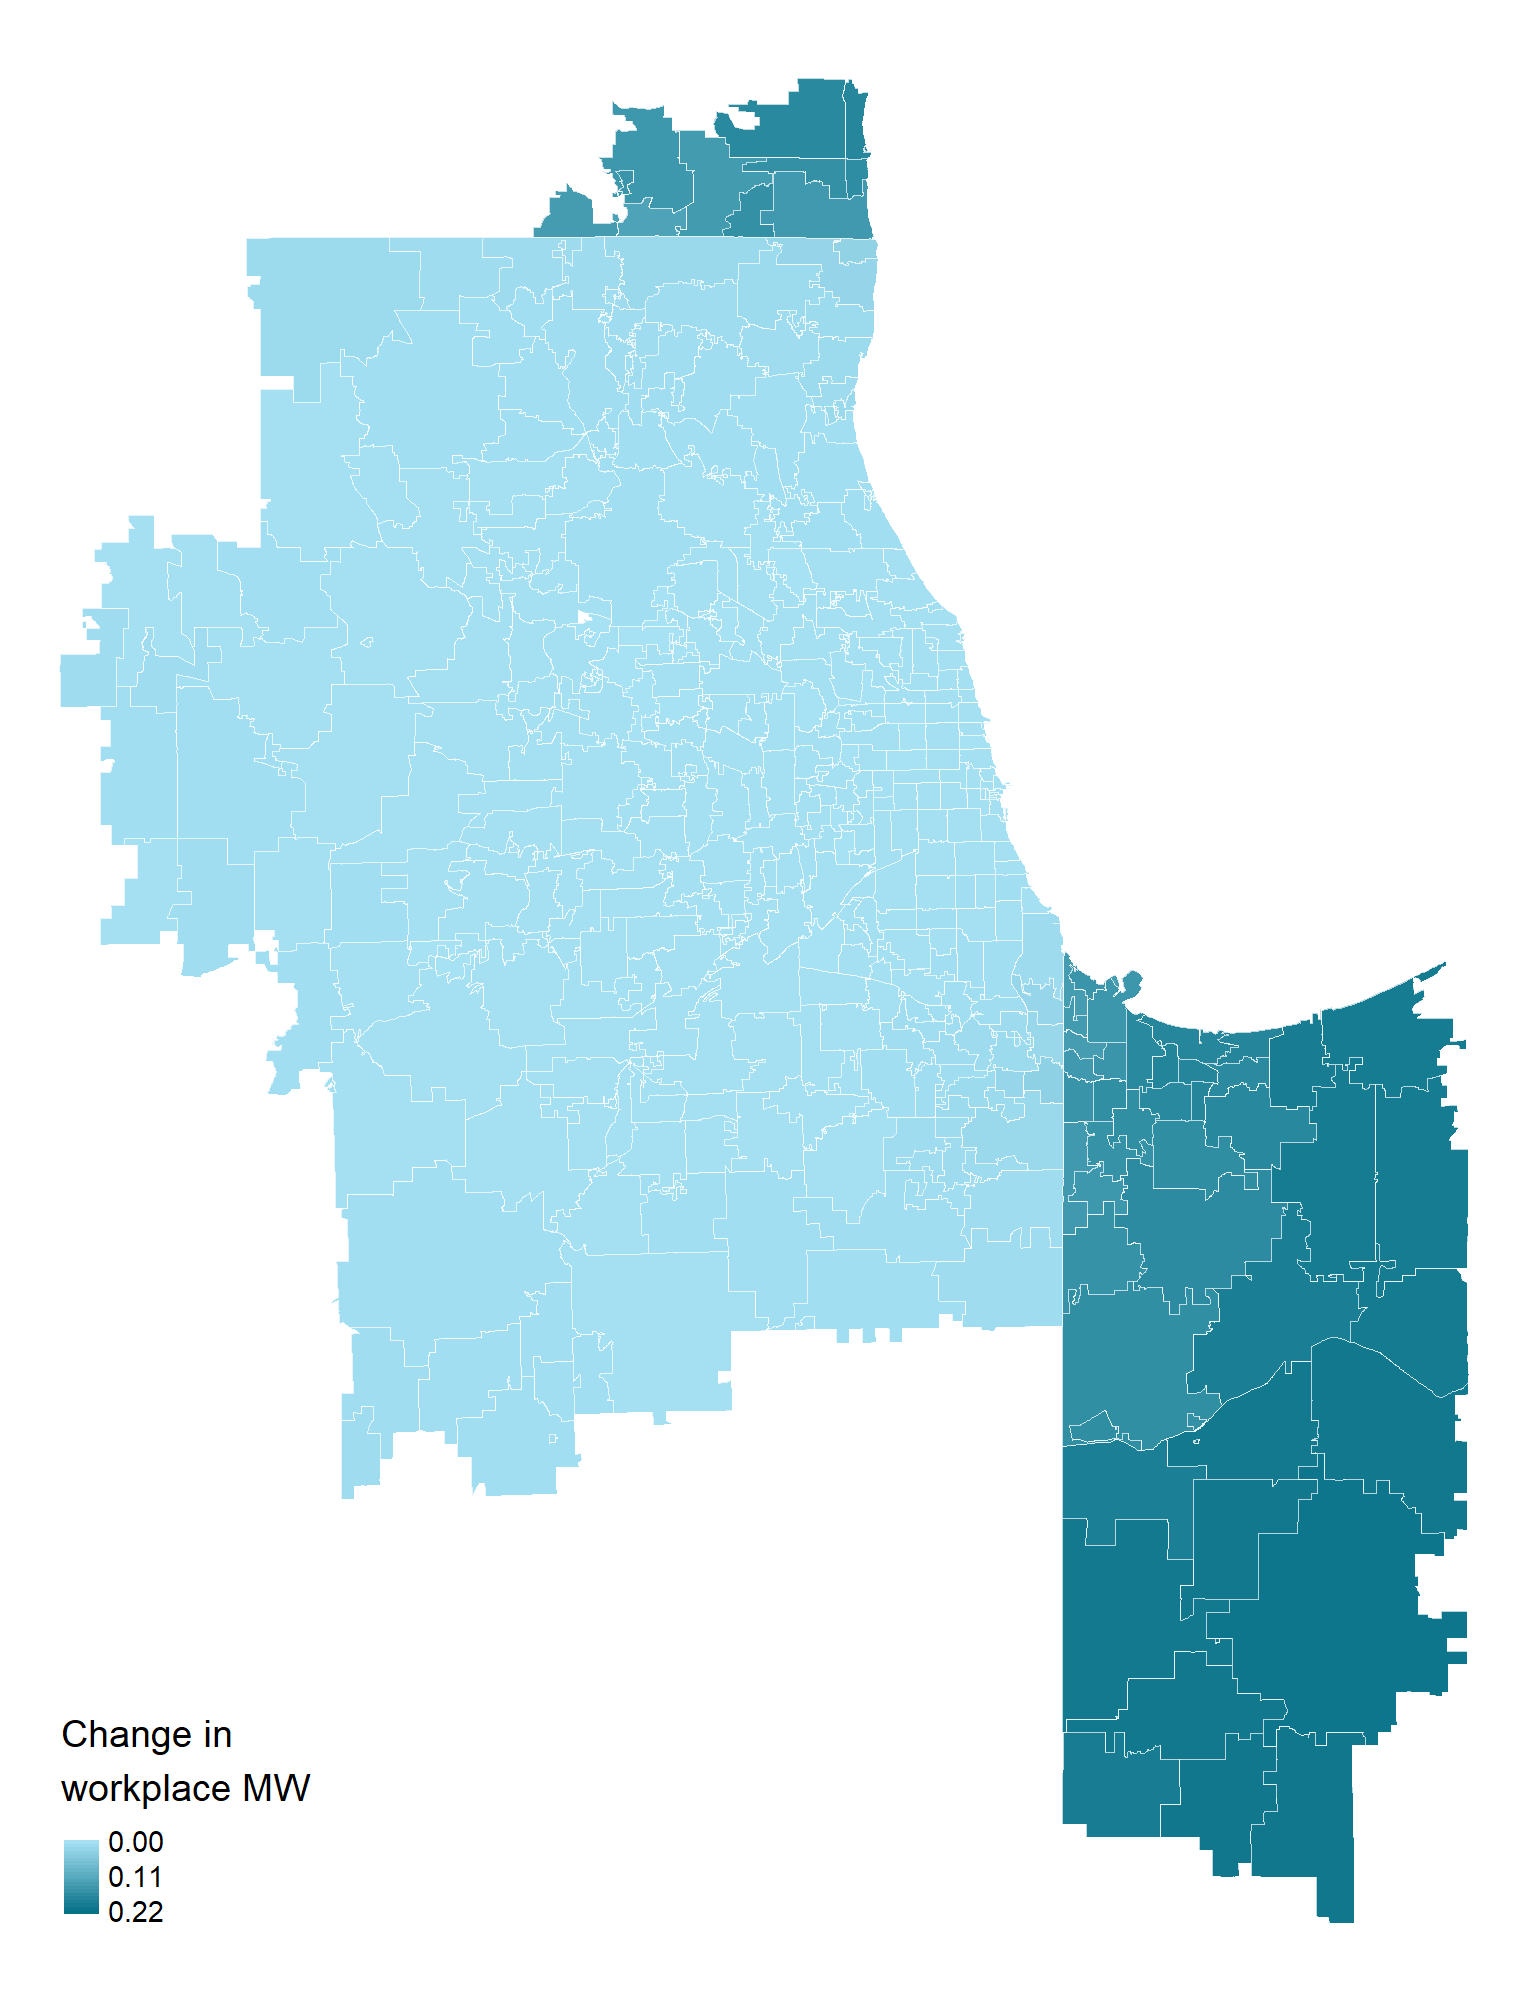
\includegraphics[width = 0.99\textwidth]{counterfactuals/output/chicago_d_mw_wkp.png}
            \caption*{Workplace MW}
        \end{subfigure}
    \end{figure}
\end{frame}

\begin{frame}
    \frametitle{Predicted increases in rents and wages}
    \begin{figure}
        \begin{subfigure}{0.51\textwidth}
            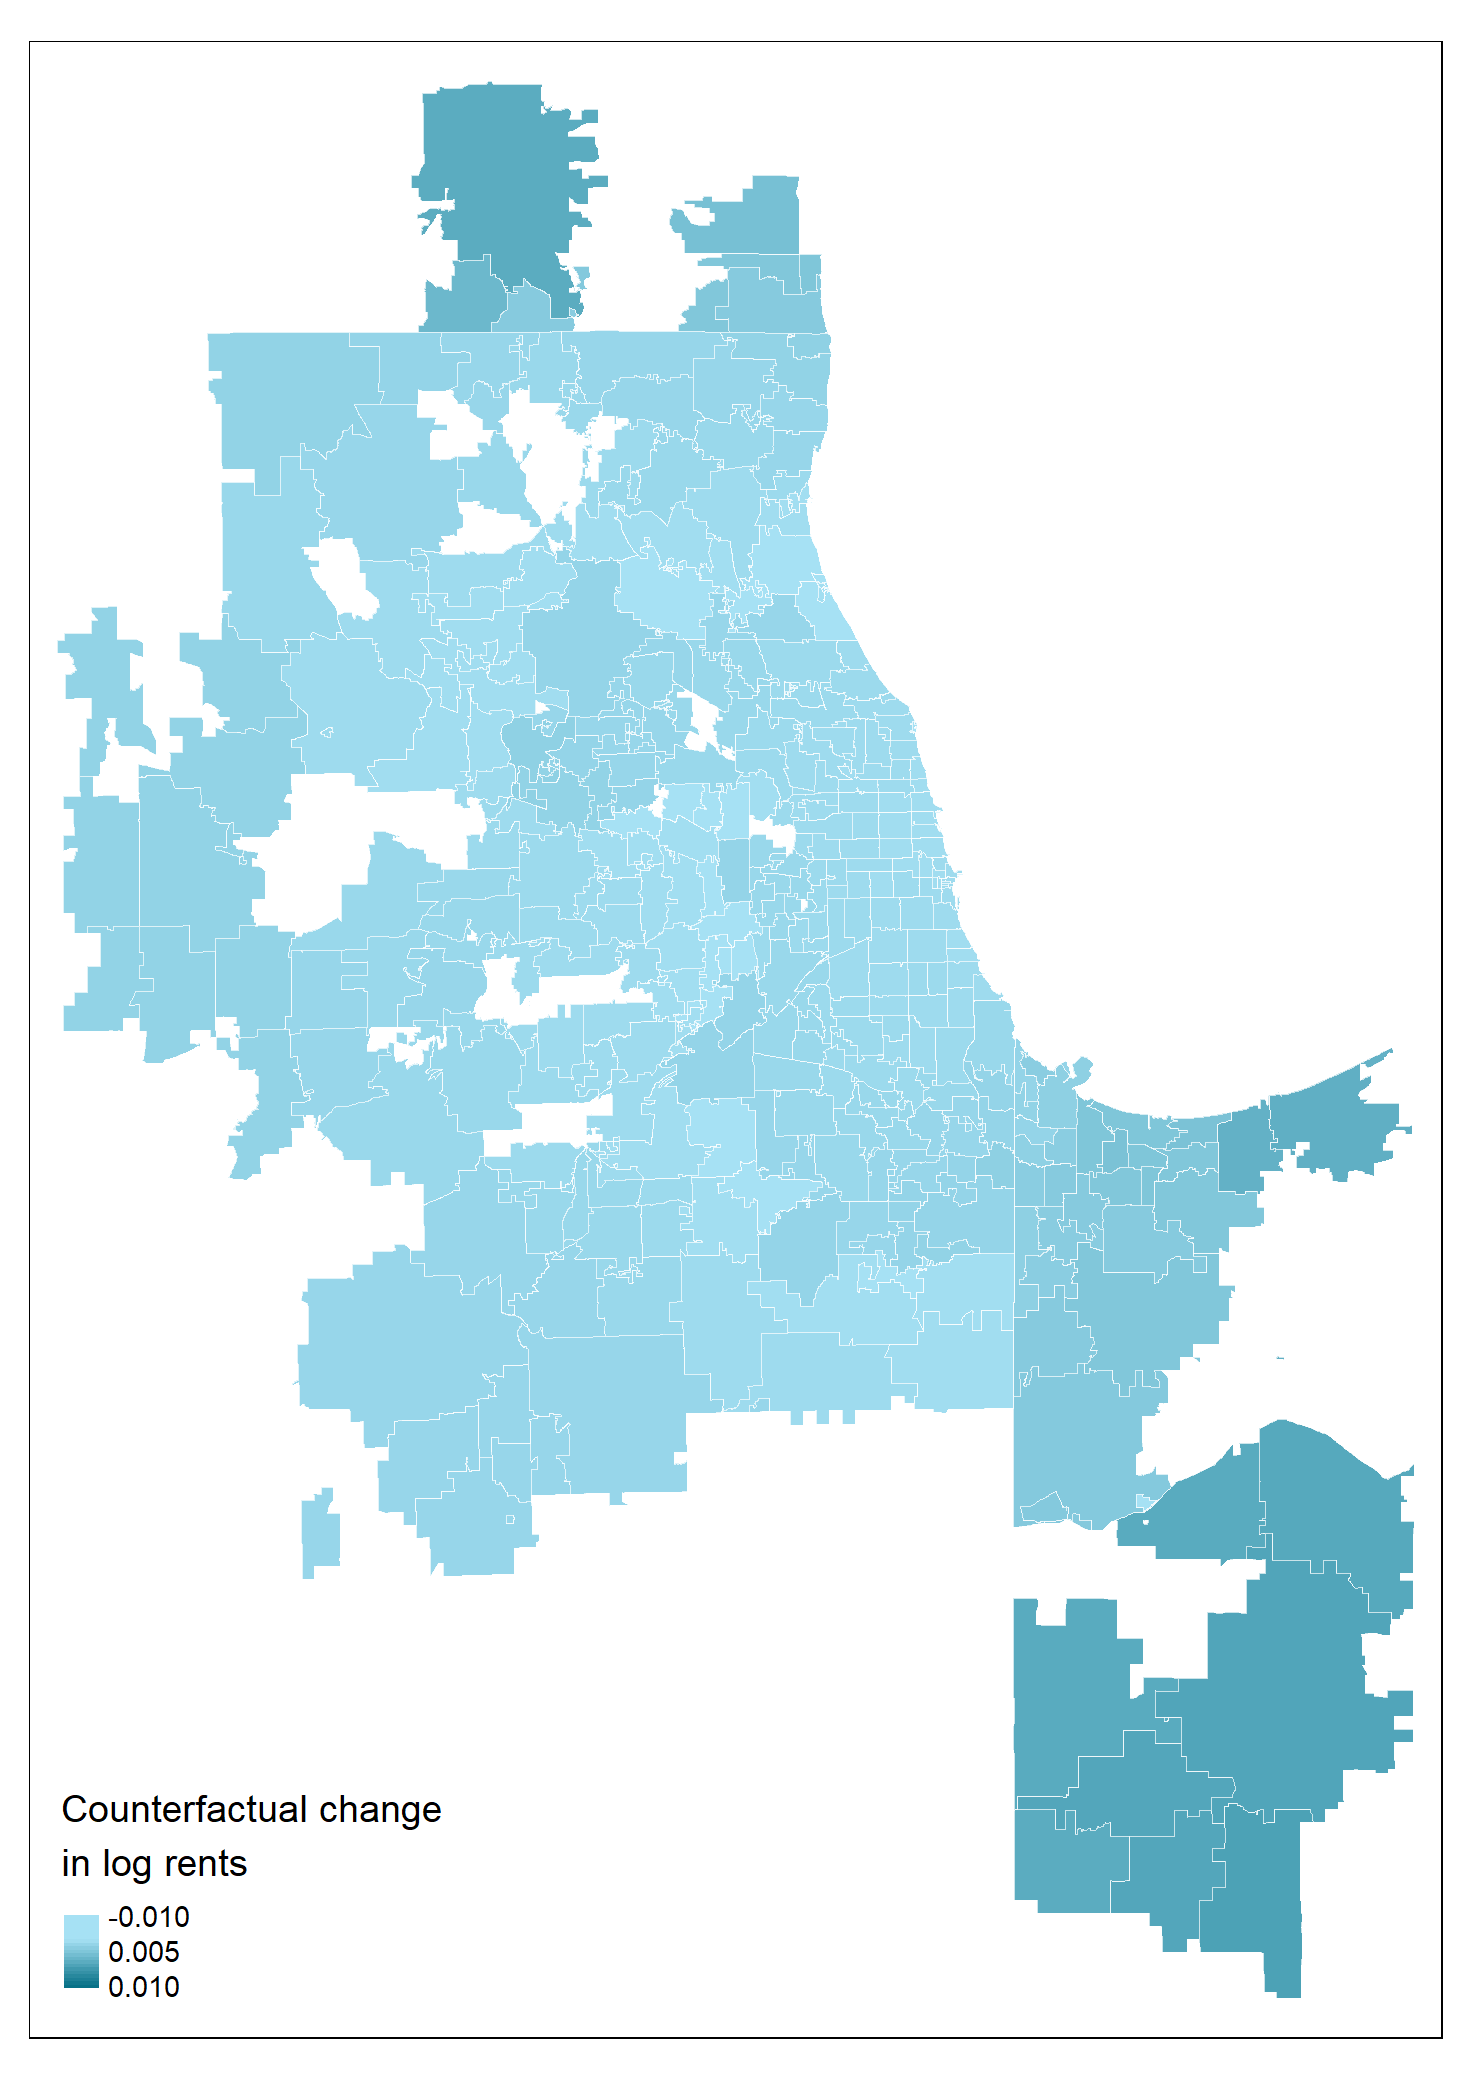
\includegraphics[width = 0.99\textwidth]{counterfactuals/output/chicago_d_ln_rents.png}
            \caption*{Predicted changes in log rents per sqft}
        \end{subfigure}%
        \begin{subfigure}{0.51\textwidth}
                         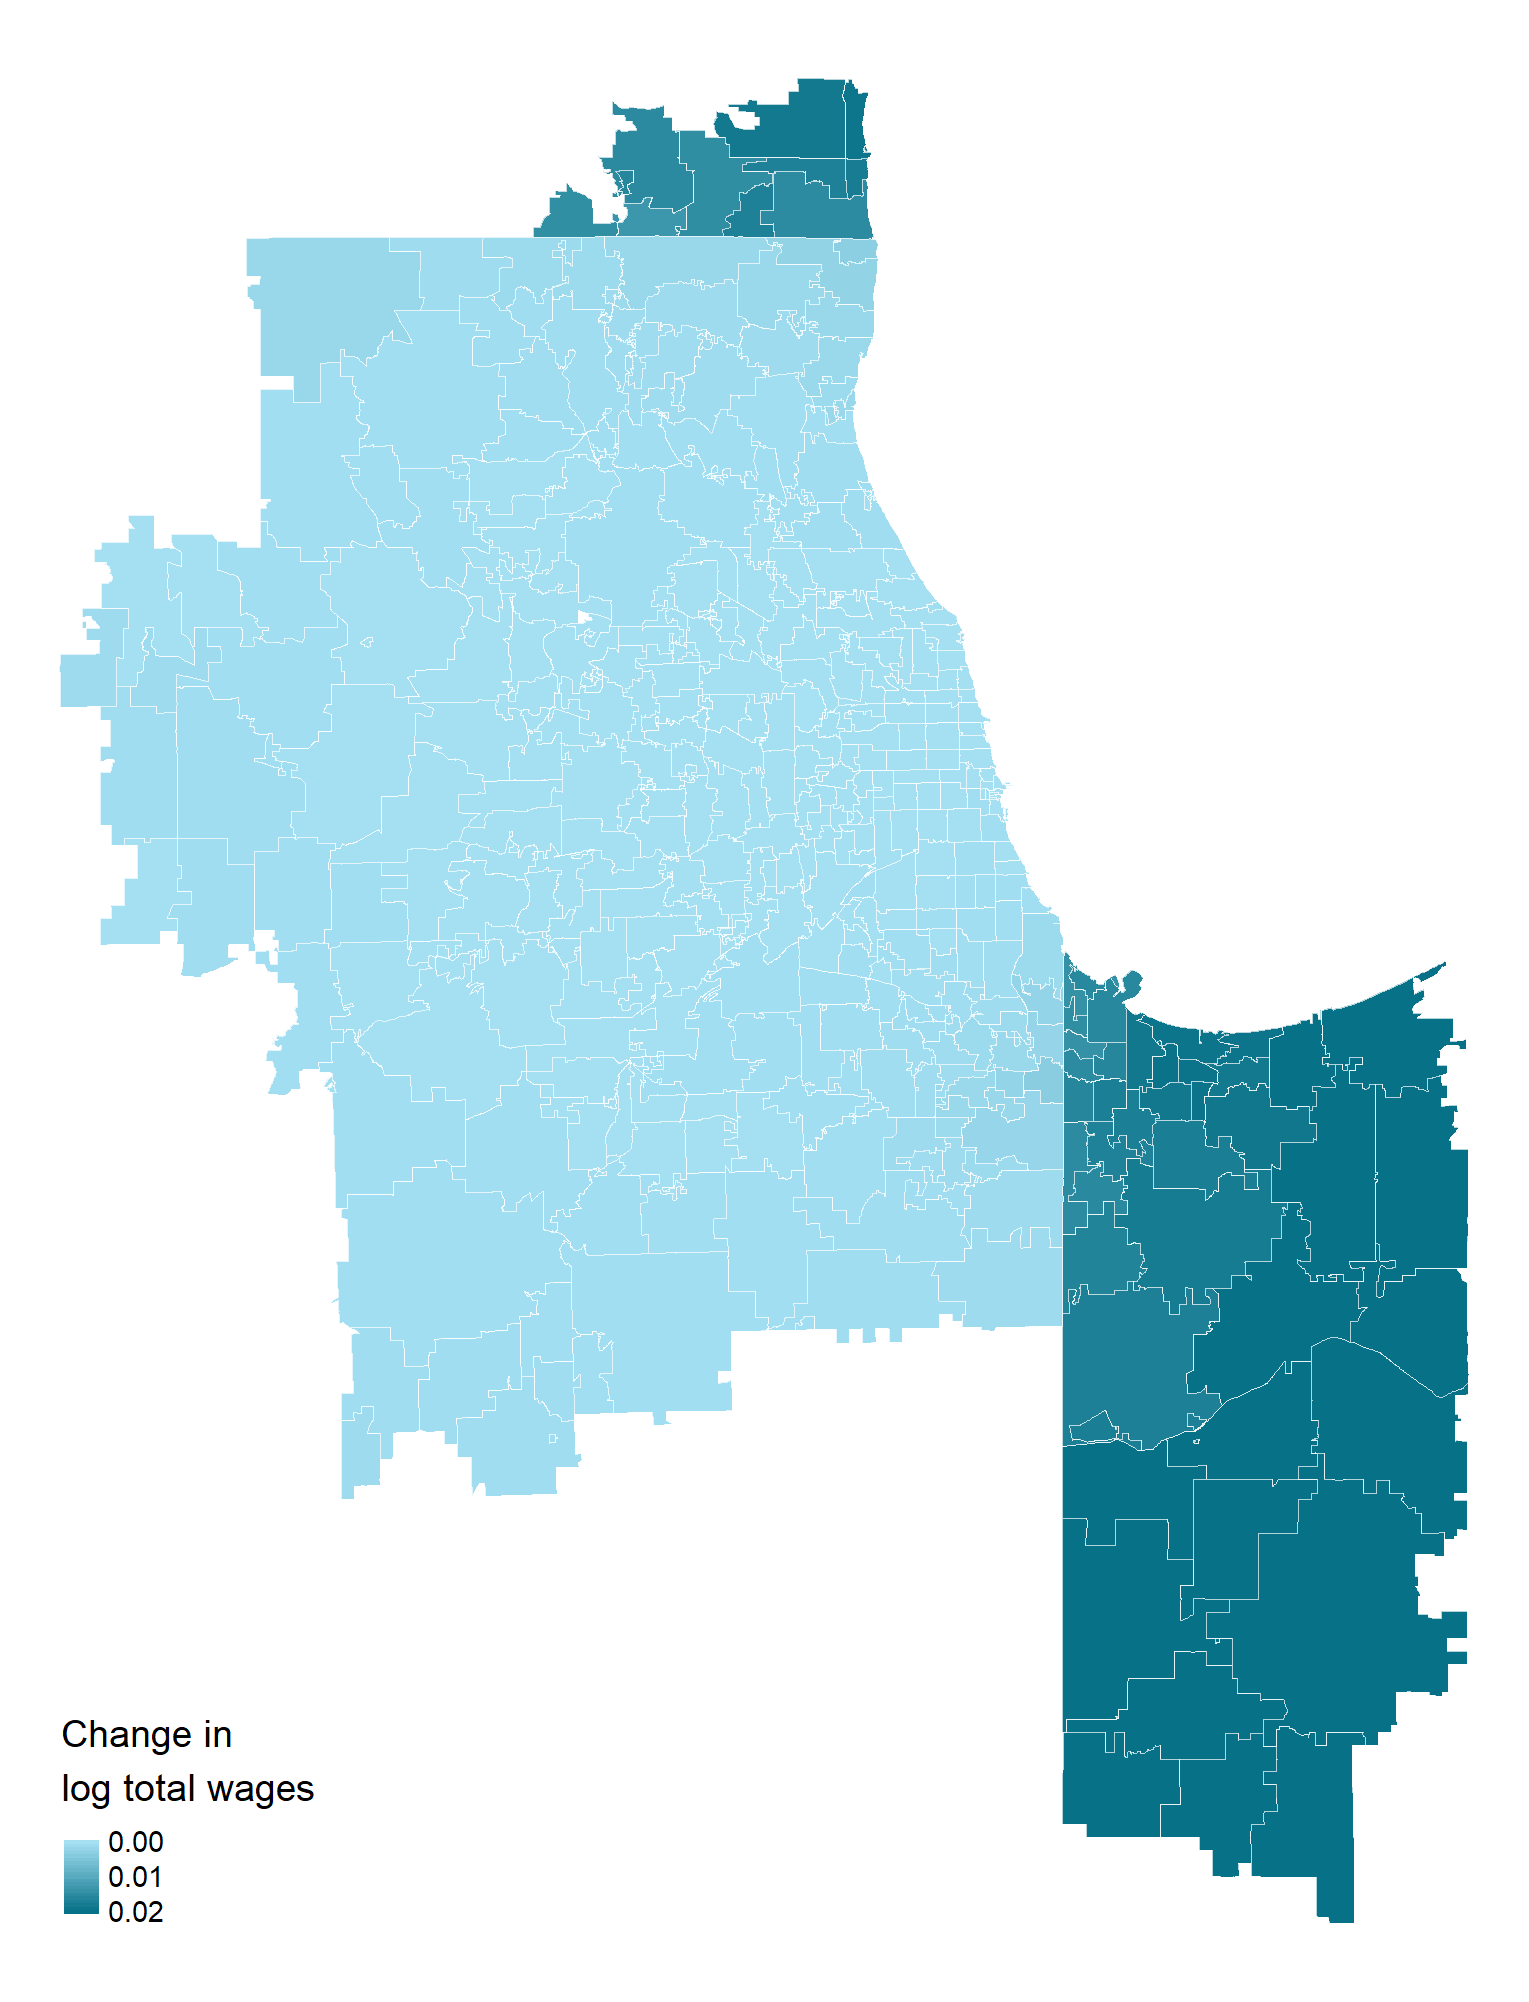
\includegraphics[width = 0.99\textwidth]{counterfactuals/output/chicago_d_ln_wagebill.png}
            \caption*{Predicted changes in log total wages}
        \end{subfigure}
    \end{figure}    
\end{frame}

\begin{frame}
    \frametitle{Predicted gradient of rent changes in the Chicago metro area}
    \begin{figure}
        \centering
        \begin{subfigure}{0.33\textwidth}
            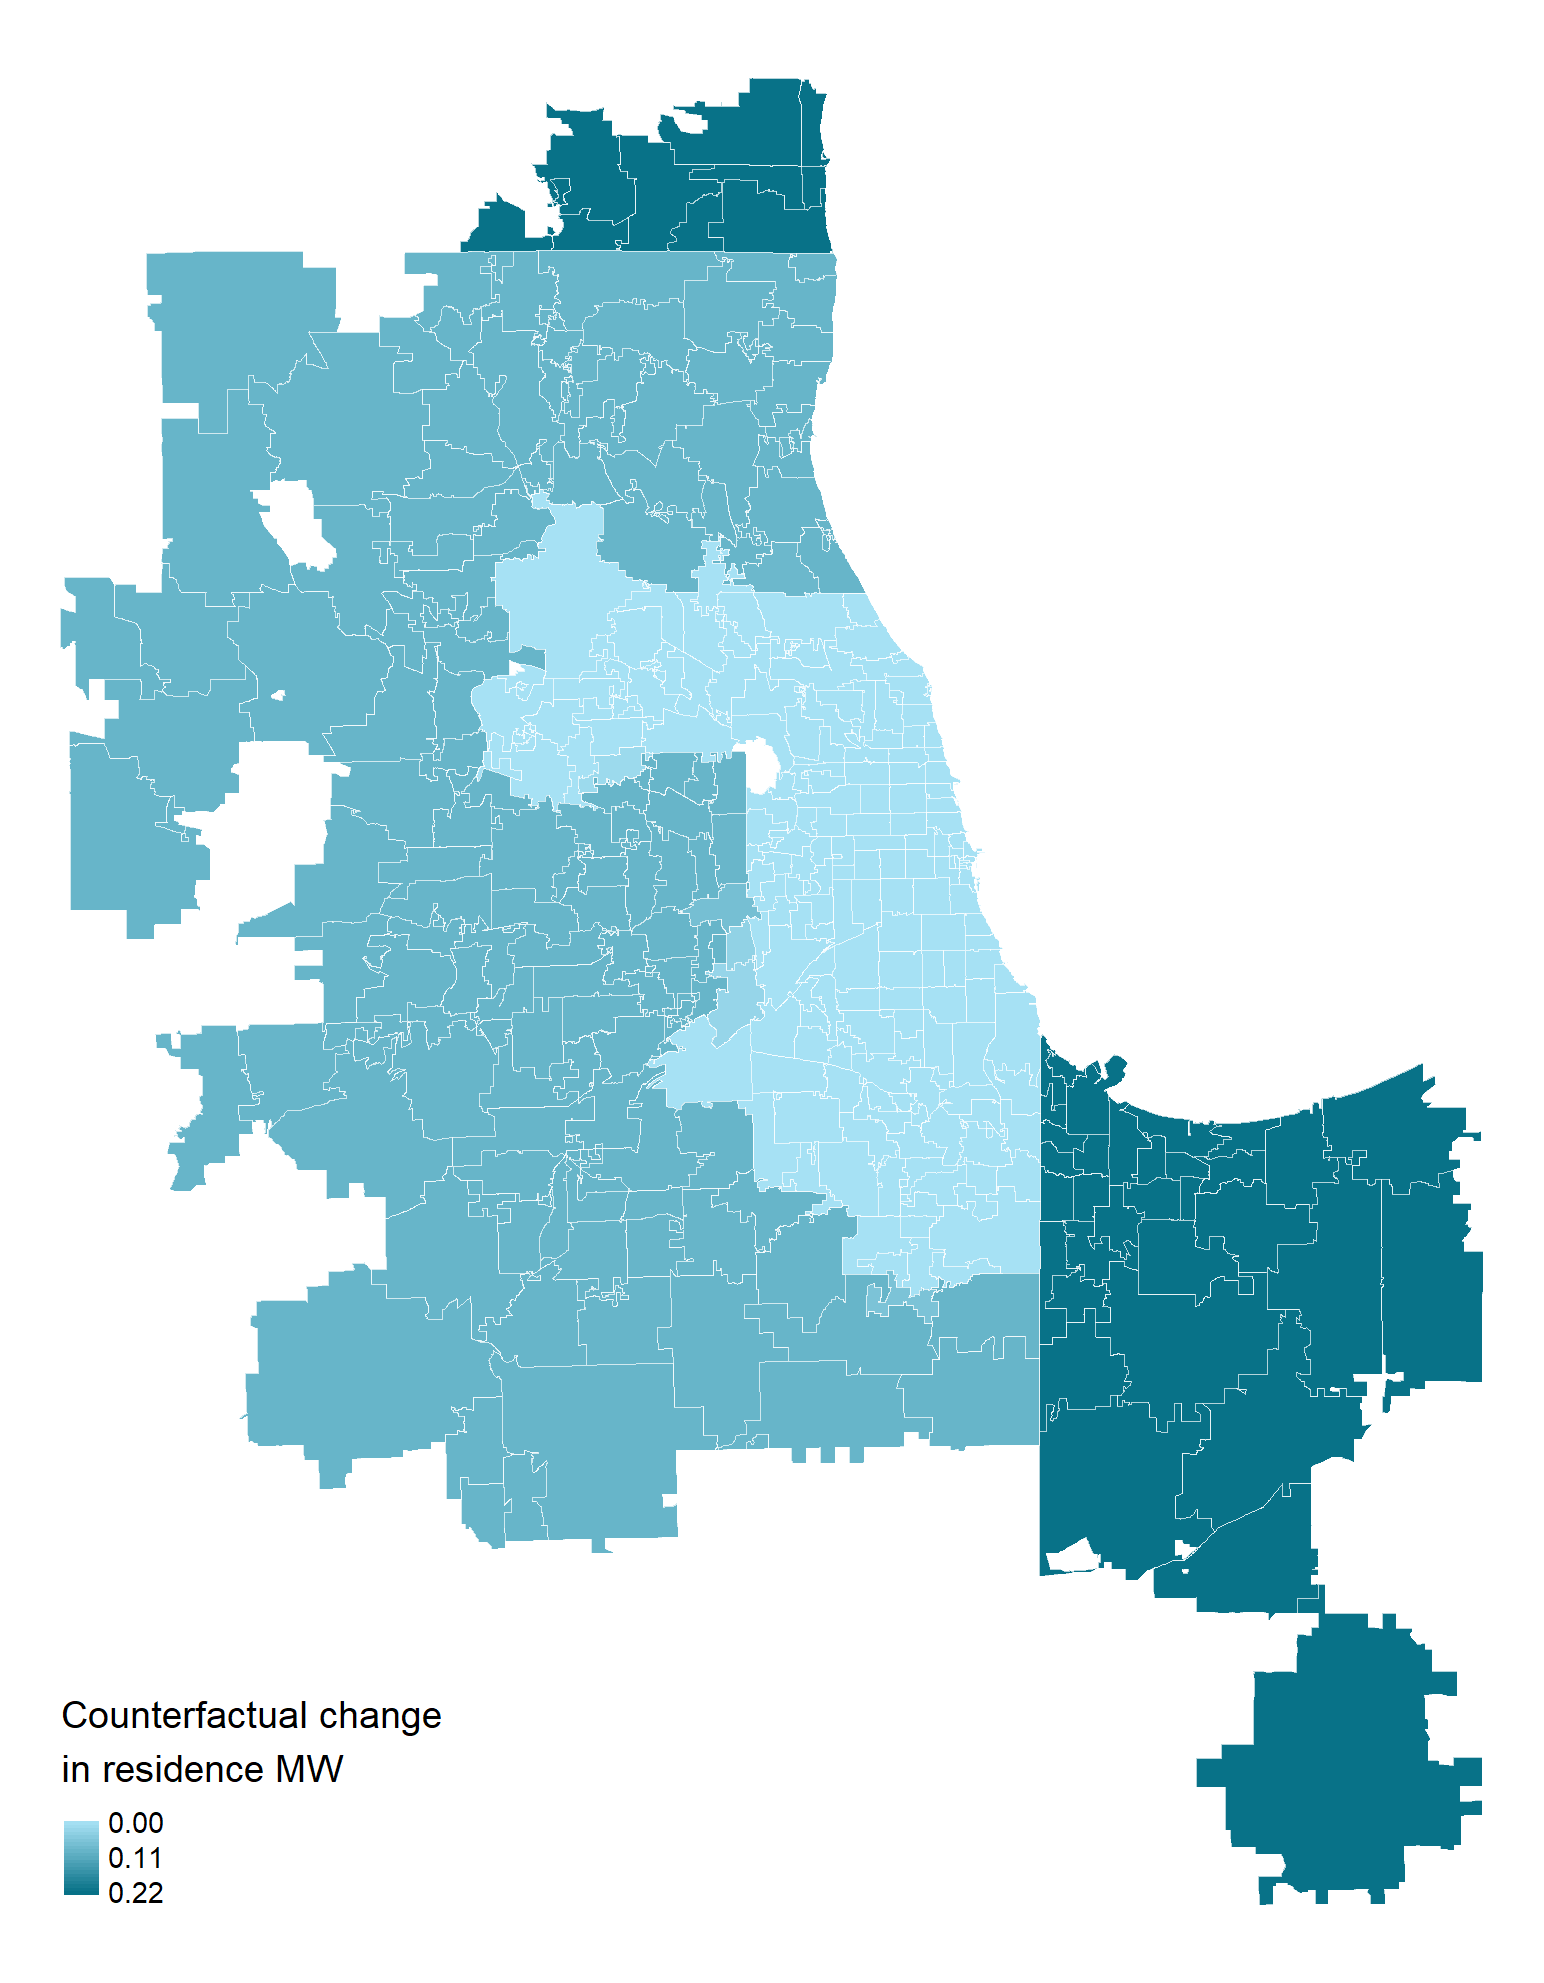
\includegraphics[width = 0.99\textwidth]{counterfactuals/output/chicago_d_mw_res.png}
            \caption*{Counterfactual change in residence MW}
        \end{subfigure}%
        \begin{subfigure}{0.33\textwidth}
                         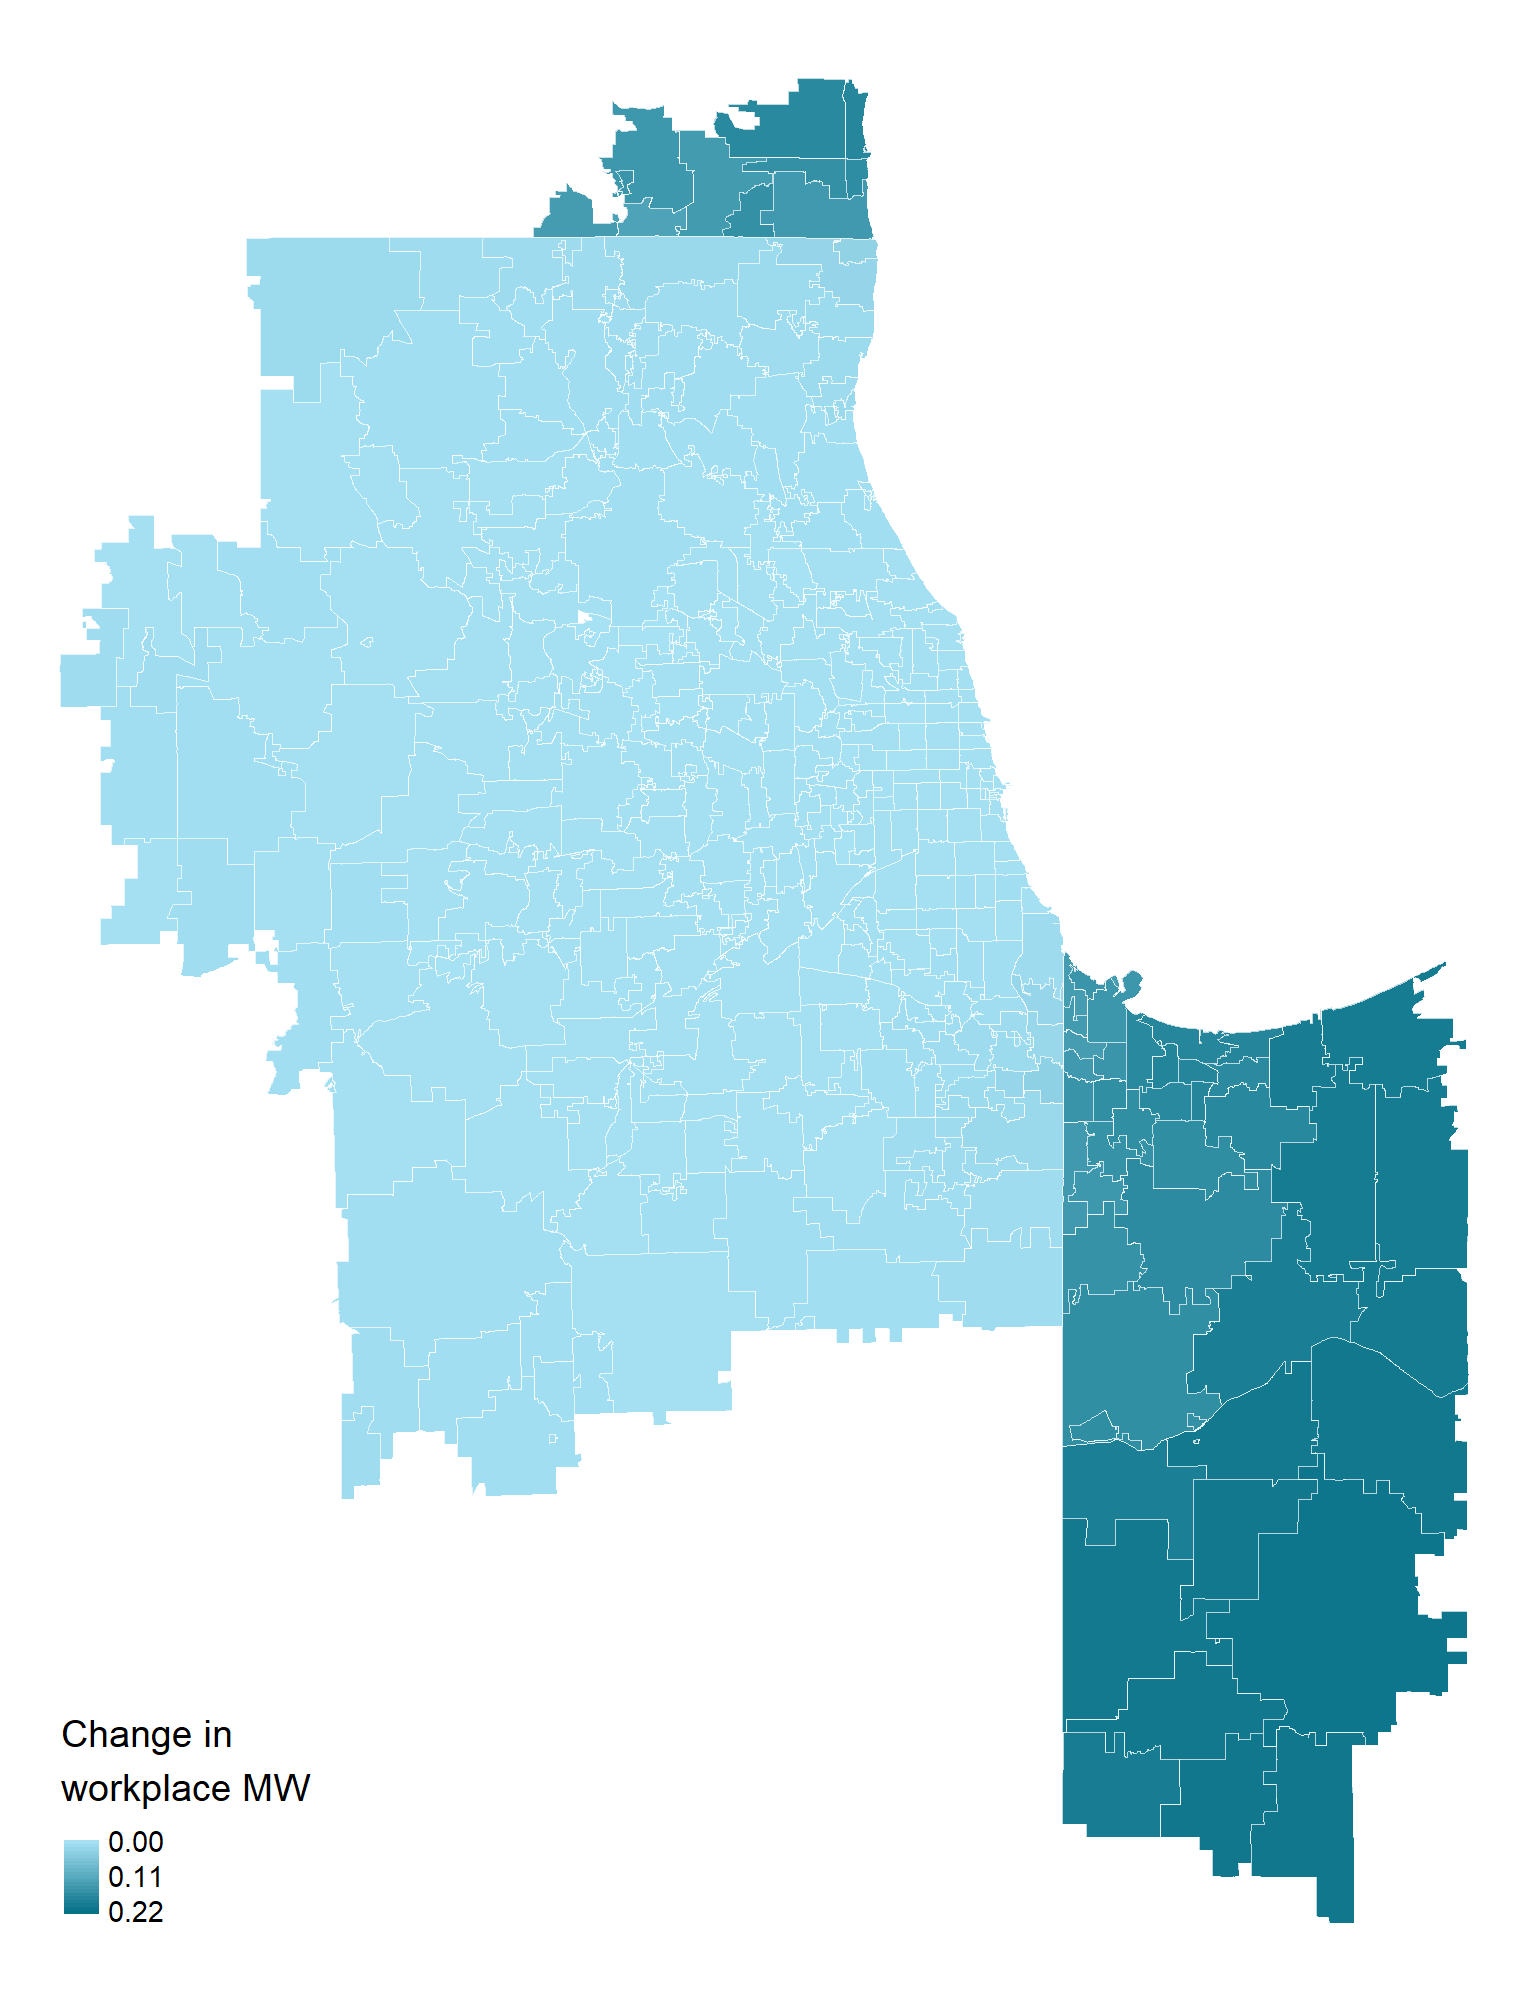
\includegraphics[width = 0.99\textwidth]{counterfactuals/output/chicago_d_mw_wkp.png}
            \caption*{Counterfactual change in workplace MW}
        \end{subfigure}
        \begin{subfigure}{0.33\textwidth}
                         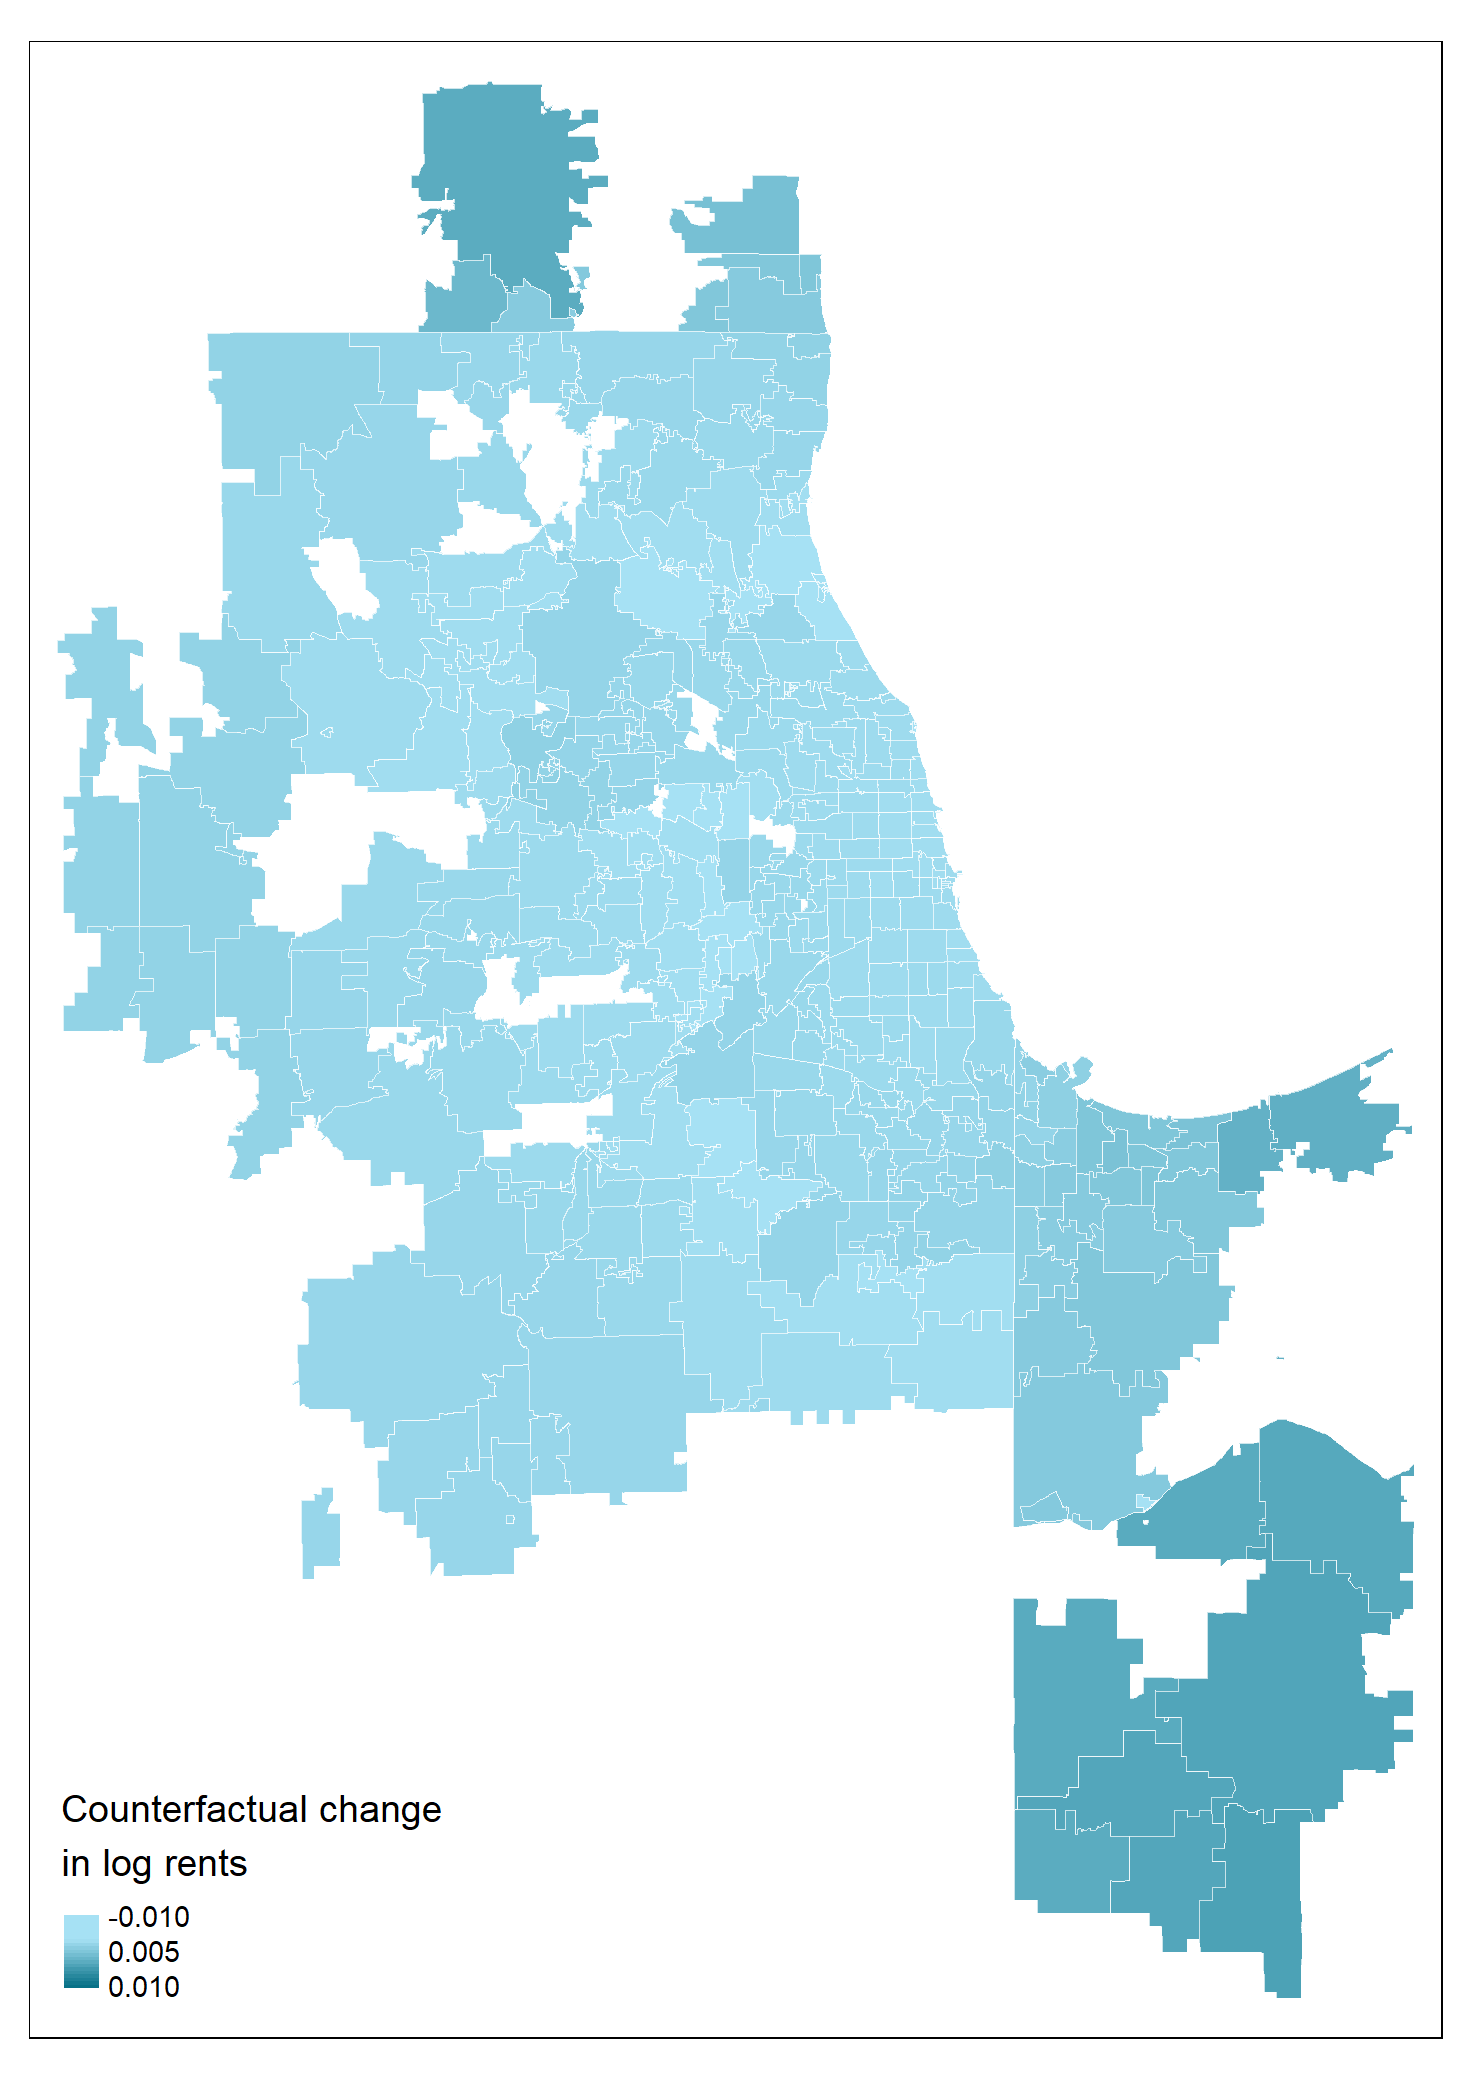
\includegraphics[width = 0.99\textwidth]{counterfactuals/output/chicago_d_ln_rents.png}
            \caption*{Counterfactual change in log rents}
        \end{subfigure}
    \end{figure}    
\end{frame}

\begin{frame}
    \frametitle{The incidence of MW changes on average}
    
    \vspace{3mm}
    %\begin{table}[]

    \label{tab:counterfactuals}
    \centering
    \scalebox{0.83}{
    \begin{tabular}{@{}lcccccc@{}}
        \toprule
                            &   & \multicolumn{2}{c}{Change in log MW}
                                    & \multicolumn{1}{c}{\multirow{2}{*}{\makecell{Ratio perc.\\increases}}} 
                                             & \multicolumn{2}{c}{Landlord share for $\alpha$}   \\ \cmidrule(lr){3-4} \cmidrule(l){6-7}
                            & N & Res.\ & Wrk.\
                                    & \multicolumn{1}{c}{}        
                                             & 0.25  & 0.45     \\ \midrule
        Effect in ZIP codes...                           &      &         &       &       &                &                 \\
        $\quad$with previous res. MW $\leq\$9\quad$    & 8,753 &  0.216   &  0.183  &  0.180  & 0.045 &  0.081   \\
        $\quad$with previous res. MW $>\$9\quad$       & 5,555 &  0   &  0.004  &  0.357  & 0.089  & 0.161   \\ \bottomrule
    \end{tabular}
    }
    \begin{minipage}{.95\textwidth} \footnotesize
        \vspace{2mm}
        Notes: The table shows computations of the pass-through share for the following
        parameters: $\beta = 0.064$, $\gamma = -0.030$, $\varepsilon = 0.180$, and $\alpha\in\{0.25, 0.45\}$.
    \end{minipage}
\end{table}


    \pause
    \vspace{3mm}

    More generally, one can think of the effect for different values of 
    $$
        \Delta \MW_i^{wrk} - \Delta \MW_i^{res}
    $$
\end{frame}

\begin{frame}
    \frametitle{The incidence of MW changes according to intensity of treatment}
    
    \begin{figure}
        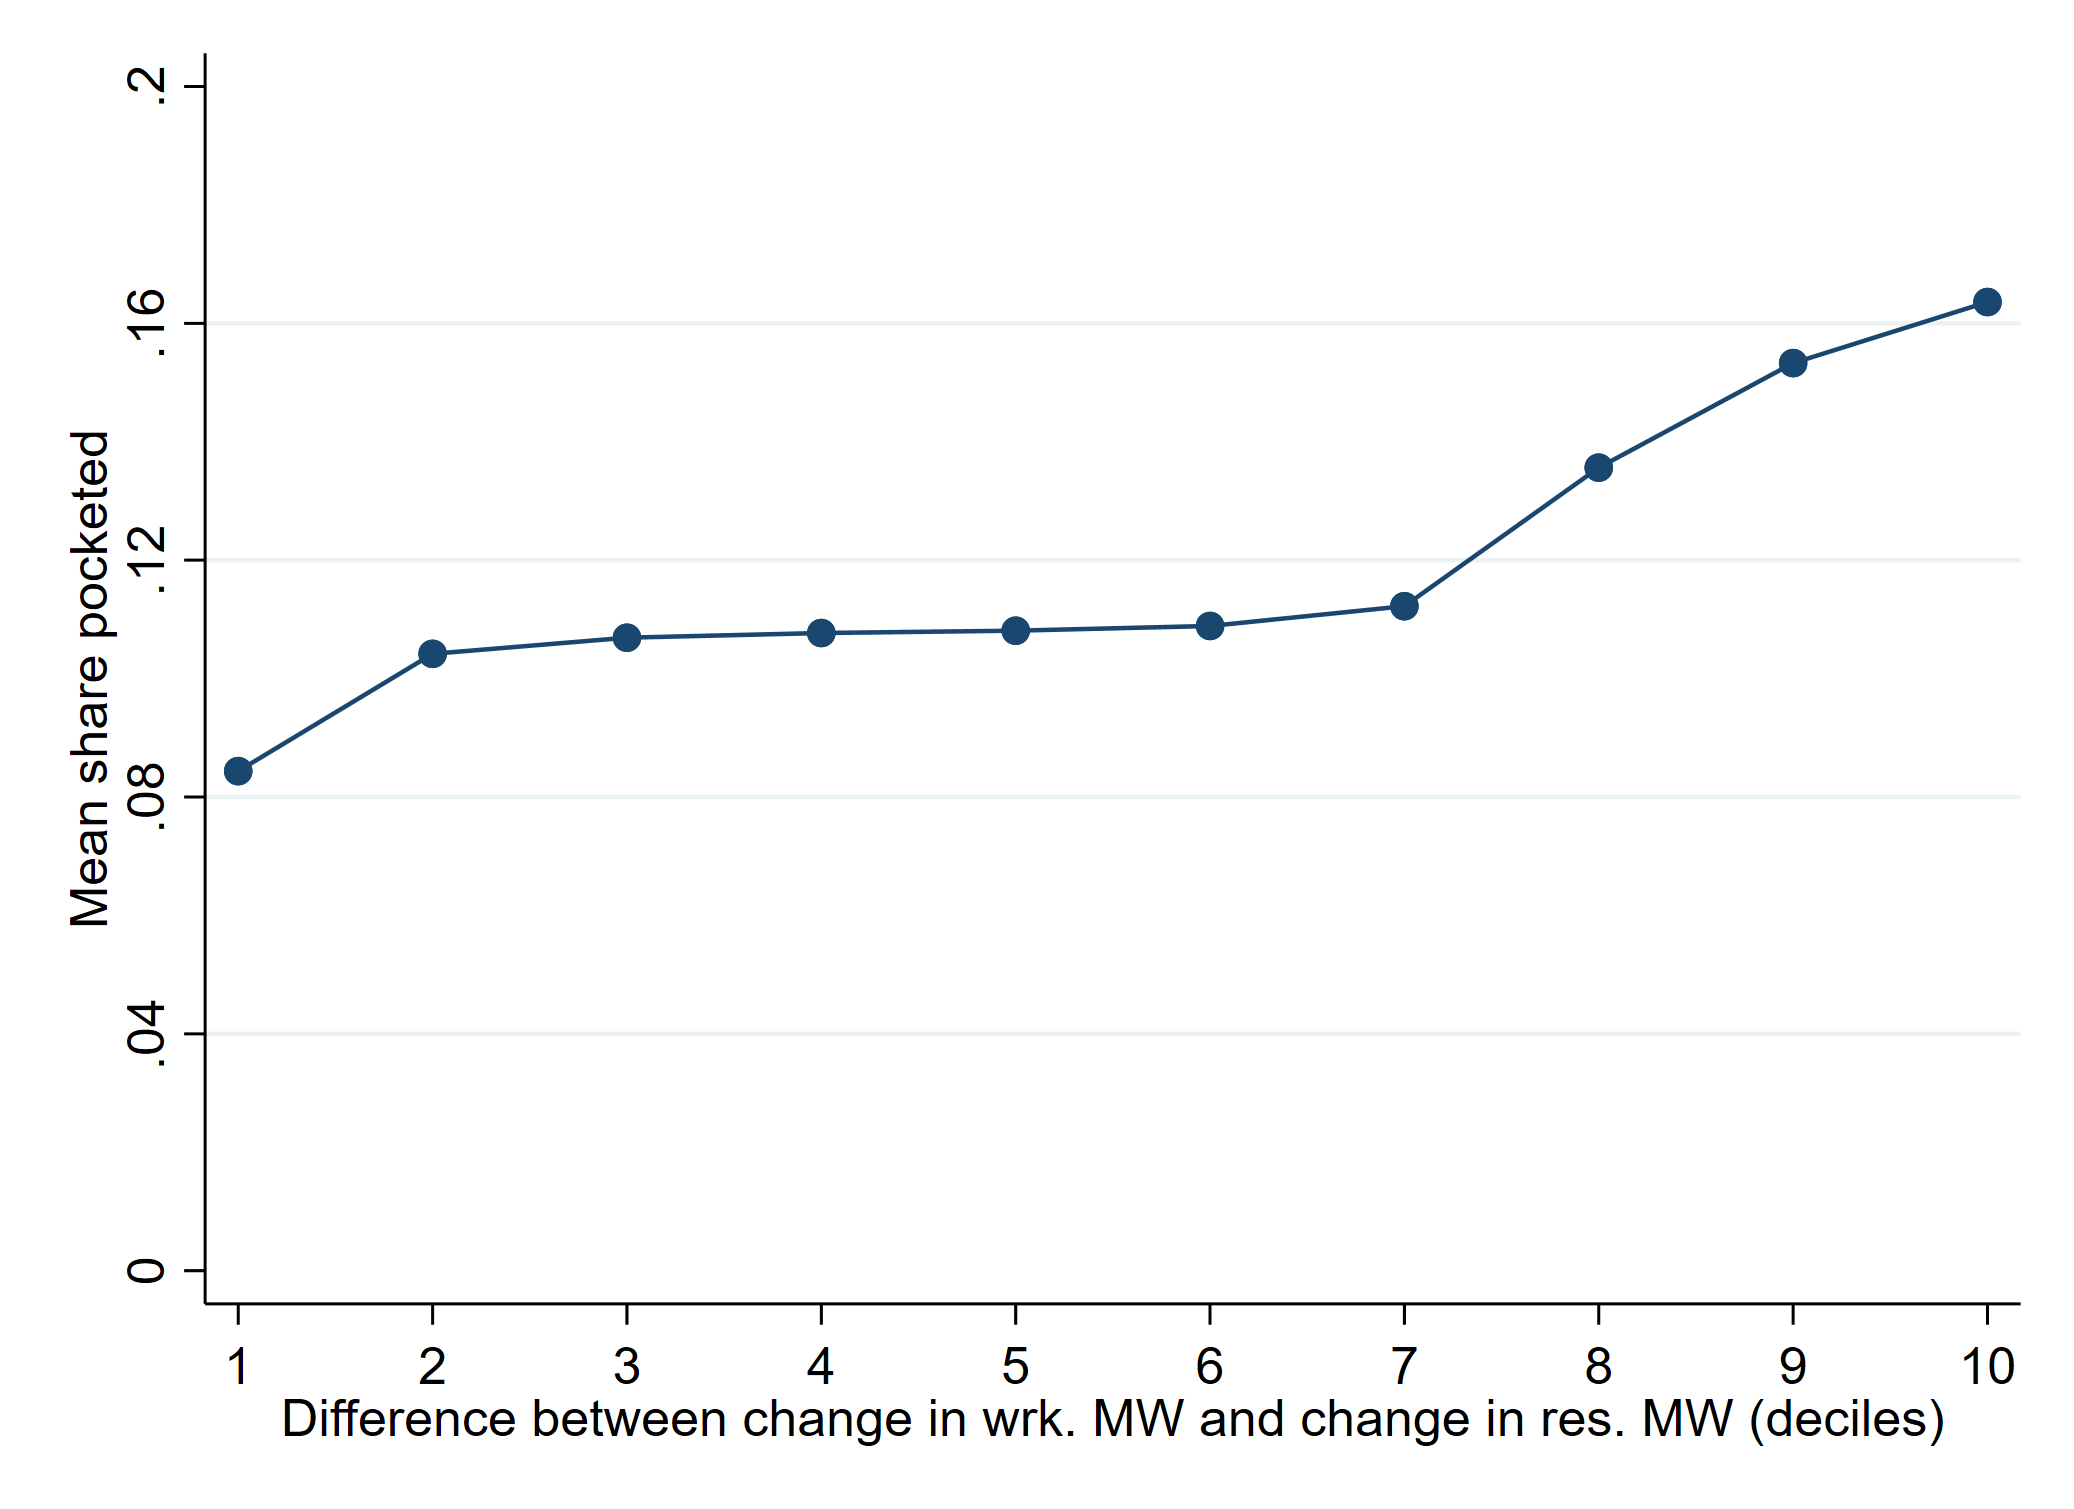
\includegraphics[width = 0.65\textwidth]{counterfactuals/output/deciles_diff.png}
        \begin{minipage}{.95\textwidth} \footnotesize
            \vspace{2mm}
            Notes: The figure shows computations of the pass-through share for the following
            parameters: $\beta = 0.064$, $\gamma = -0.030$, $\varepsilon = 0.180$, and $\alpha=0.35$.
        \end{minipage}
    \end{figure}
\end{frame}

%%%%%%%%%%%%%%%%%%%%%%%%%%%%%%%%%%%%%%%%%%%%%%%%%%%%%%%%%%%%%%%%%%%%%%%%%%%%%%%%
\section{Concluding remarks}

\begin{frame}
    \frametitle{Conclusion}
    
    \begin{itemize}
        \item When studying effects of place-based policies on the housing market it is crucial
         to account for the fact that agents live and work in different locations.
         \vspace{1mm}
         \item We estimate an elasticity of workplace MW to rents of about $0.065$, and of residence MW of $-0.03$.
         \vspace{1mm}
         \item Our estimates imply that landlords pocket between 5 and 15 cents cents on the dollar of the extra 
         income that MW policies put on the table.
         \vspace{1mm}
         \item Landlords in areas right outside of where the MW policies are implemented are those that are set to extract the most rents. 
         \item Even with a two-parameter model, we are able to describe and predict rich patterns in the rental markets.
    \end{itemize}
    
\end{frame}

\begin{frame}[c]
    \begin{center}
        \Large Thank You!
    \end{center}
\end{frame}

%%%%%%%%%%%%%%%%%%%%%%%%%%%%%%%%%%%%%%%%%%%%%%%%%%%%%%%%%%%%%%%%%%%%%%%%%%%%%%%%%%%%%%%%%%
%                                       APPENDIX                                        %
%%%%%%%%%%%%%%%%%%%%%%%%%%%%%%%%%%%%%%%%%%%%%%%%%%%%%%%%%%%%%%%%%%%%%%%%%%%%%%%%%%%%%%%%%%

\appendix

\renewcommand\thetable{\thesection.\arabic{table}}
\renewcommand\thefigure{\thesection.\arabic{figure}} 
\setcounter{table}{0}
\setcounter{figure}{0}

\section{Appendix}

\begin{frame}[label = nyc_example]
\frametitle{New York (MW changes in January 2019)}
    \begin{columns}
        \begin{column}{0.50\textwidth}
            \vspace{-4mm}
            \begin{figure}
                \centering
                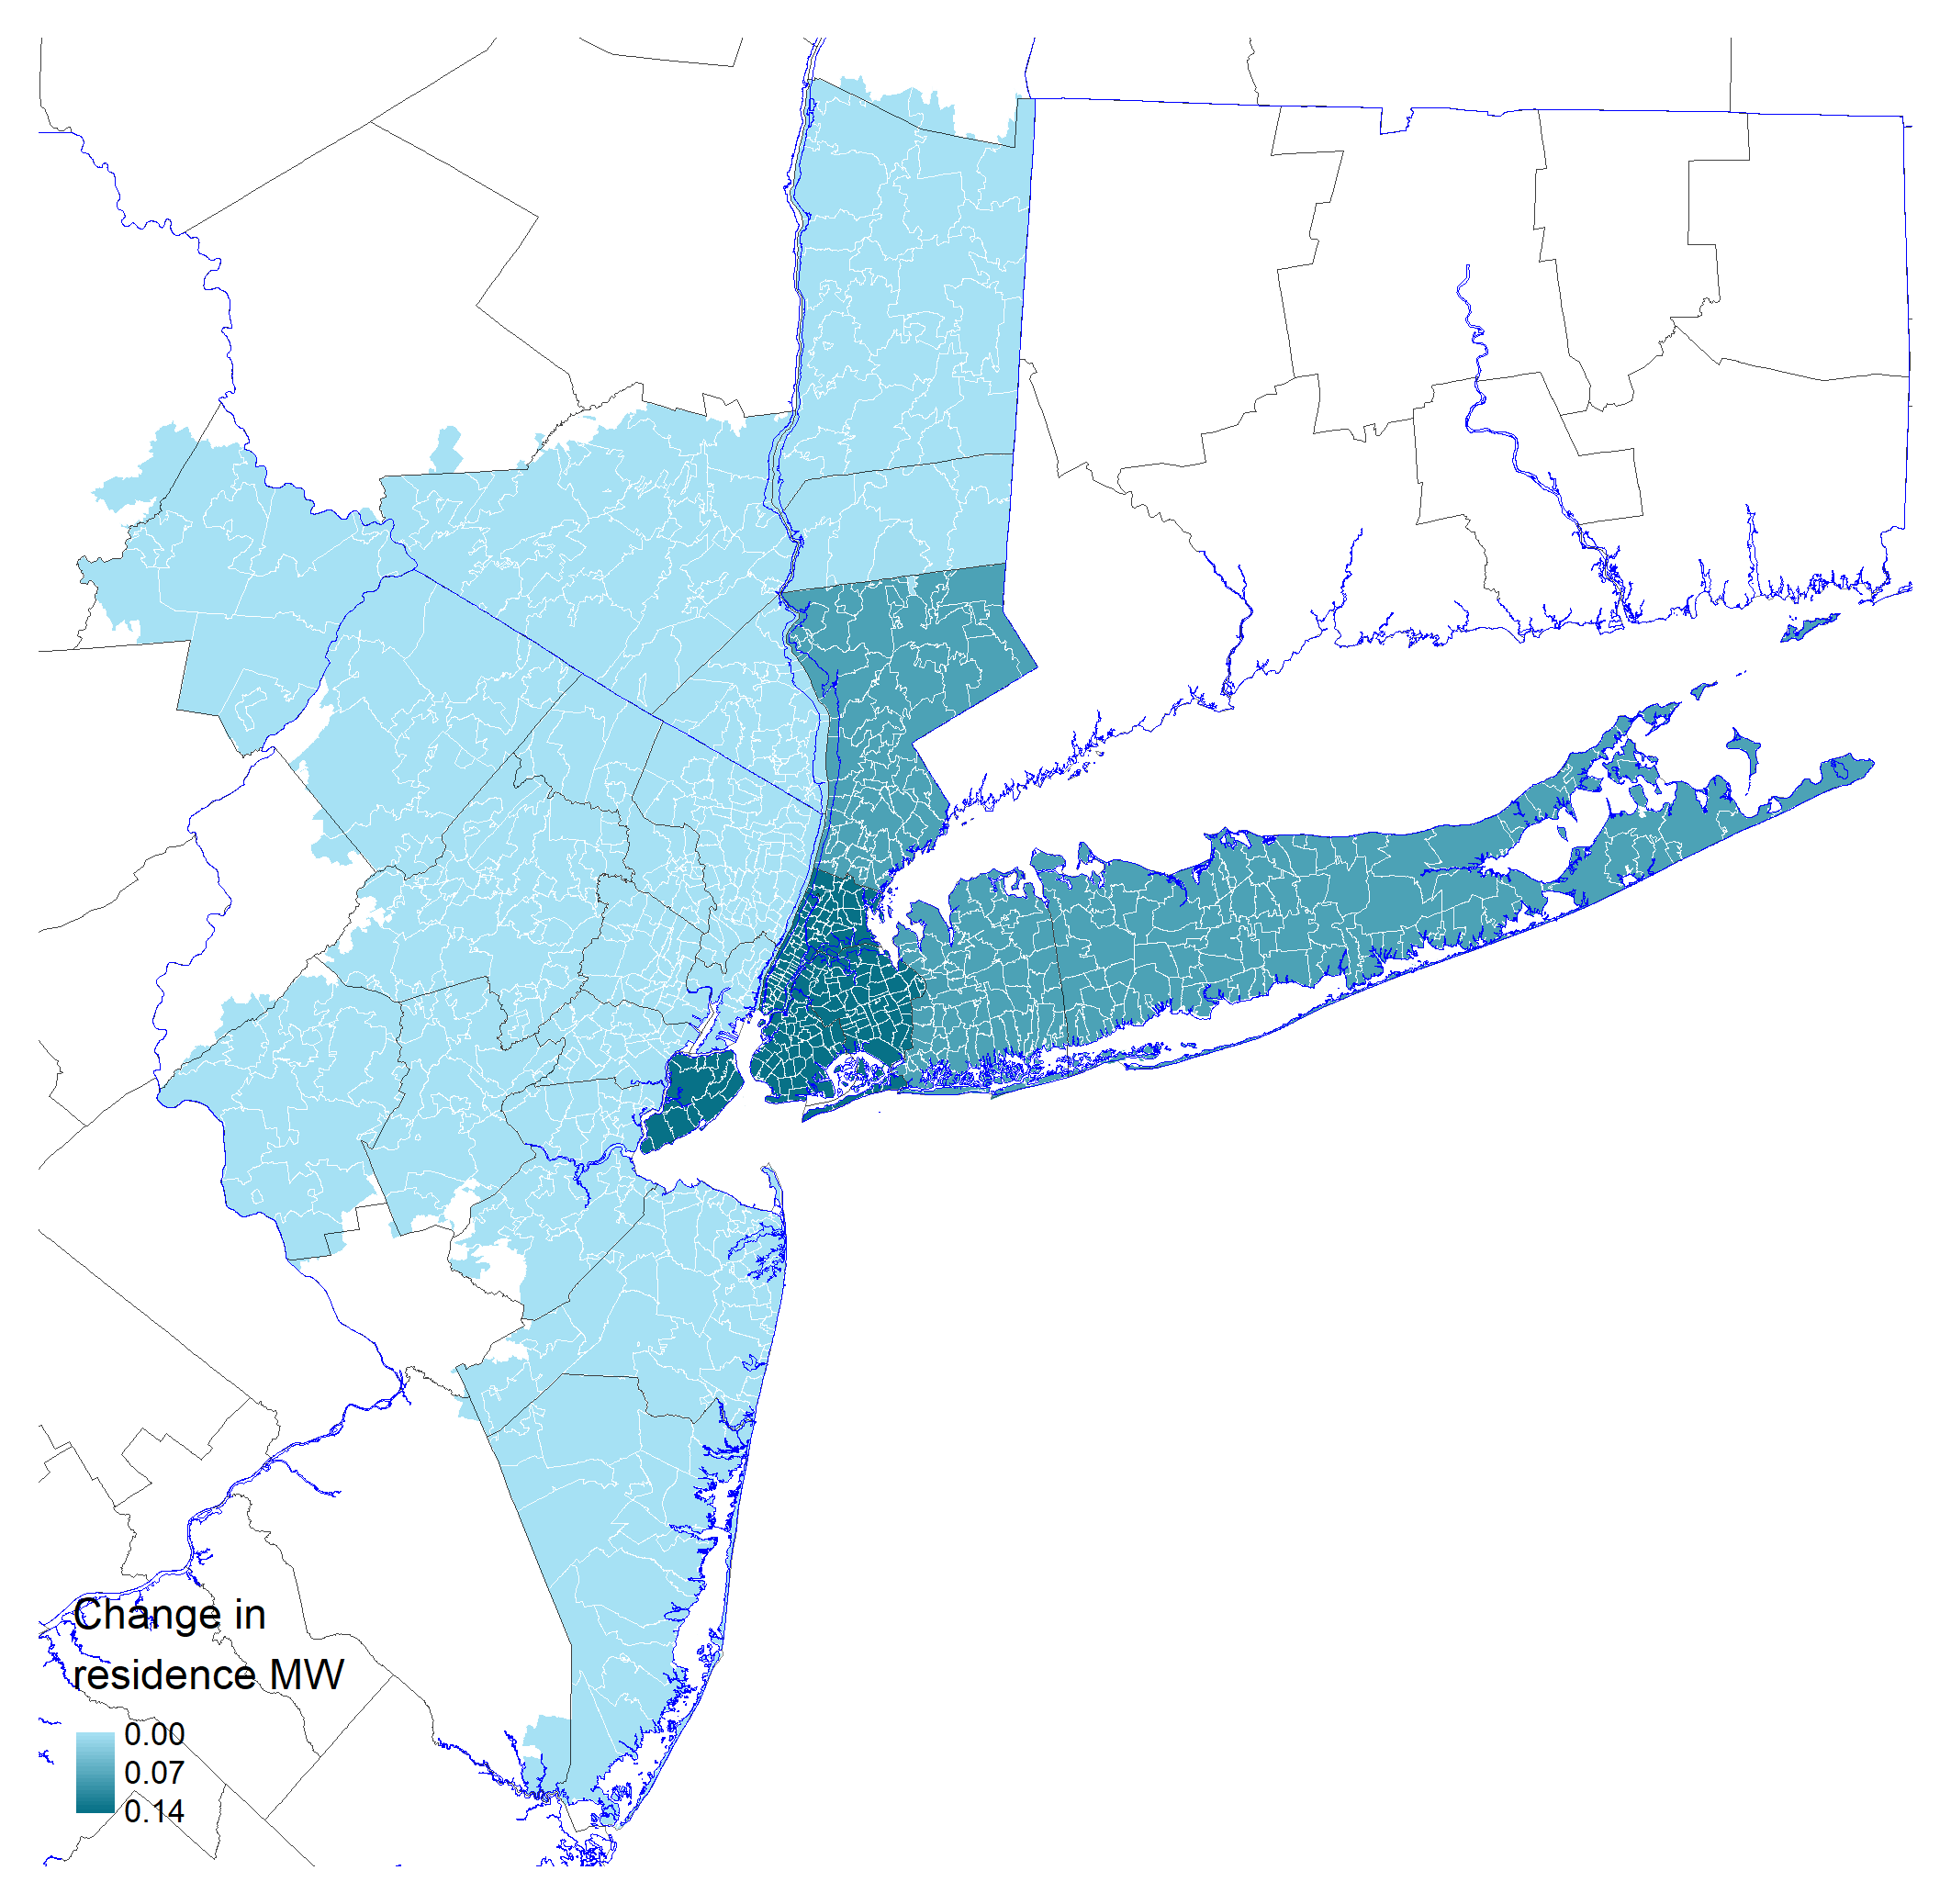
\includegraphics[scale = 0.36]{maps_events/output/nyc_2018-12_statutory_mw.png}
            \end{figure}   
        \end{column}
        \begin{column}{0.50\textwidth}
            \vspace{-4mm}
            \begin{figure}
                \centering
                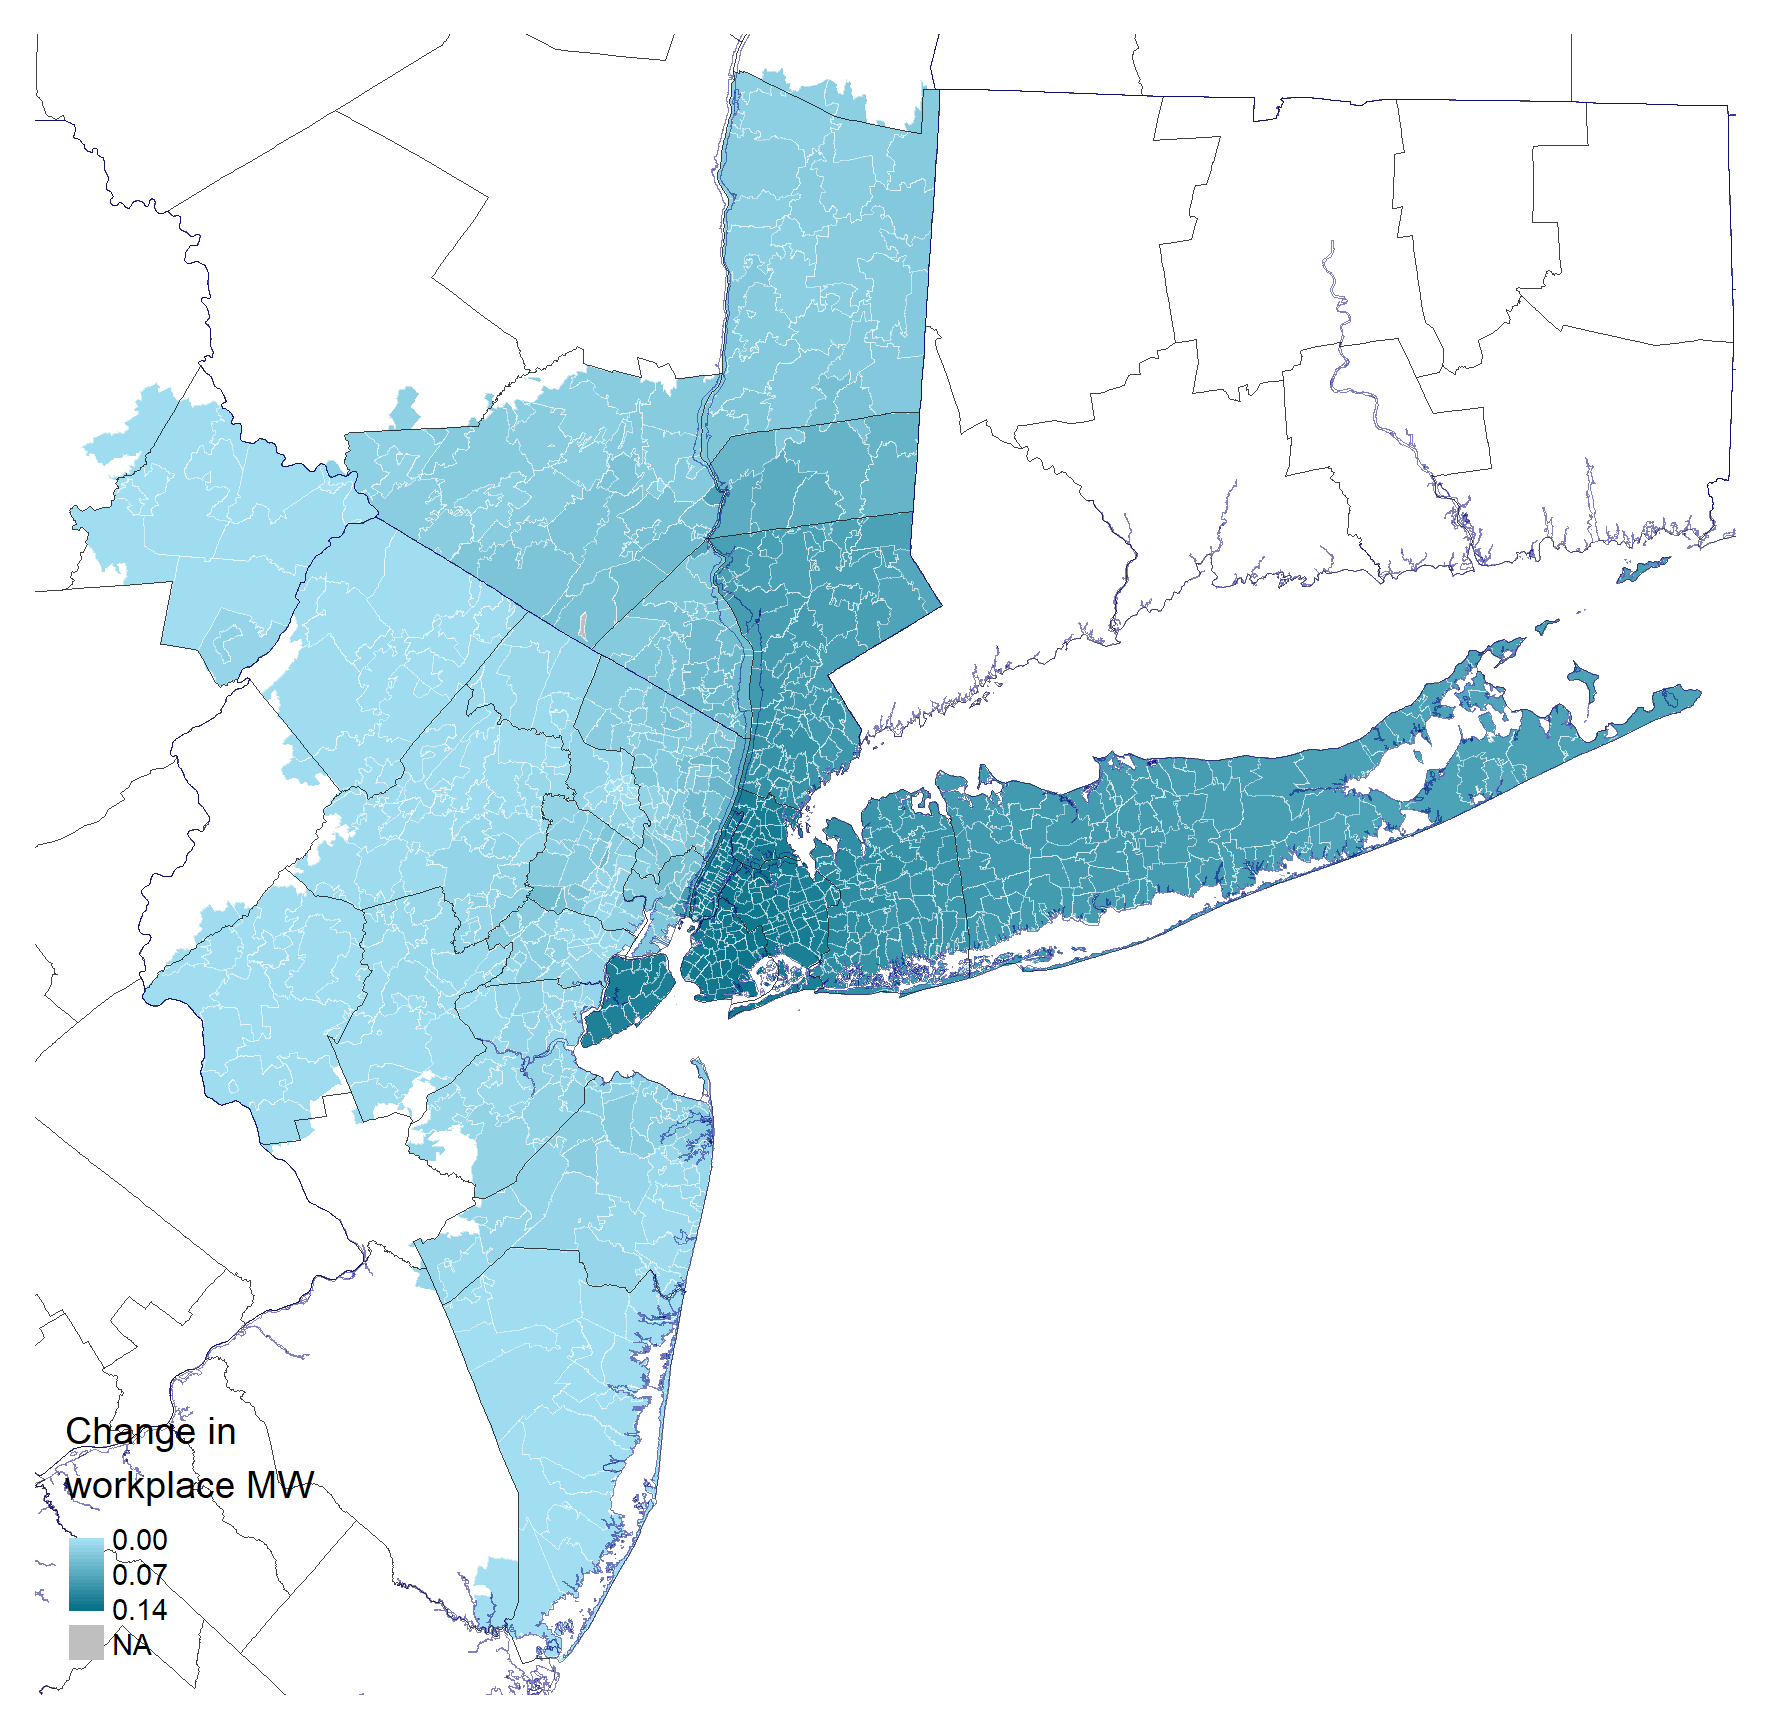
\includegraphics[scale = 0.36]{maps_events/output/nyc2018-12_wkp_mw.png}
            \end{figure}   
        \end{column}
    \end{columns}
    \hyperlink{chi_example}{\beamerbutton{Go back}}
\end{frame}

\begin{frame}[label = bay_example]
\frametitle{Bay area (MW changes in January 2019)}
    \begin{columns}
        \begin{column}{0.50\textwidth}
            \vspace{-4mm}
            \begin{figure}
                \centering
                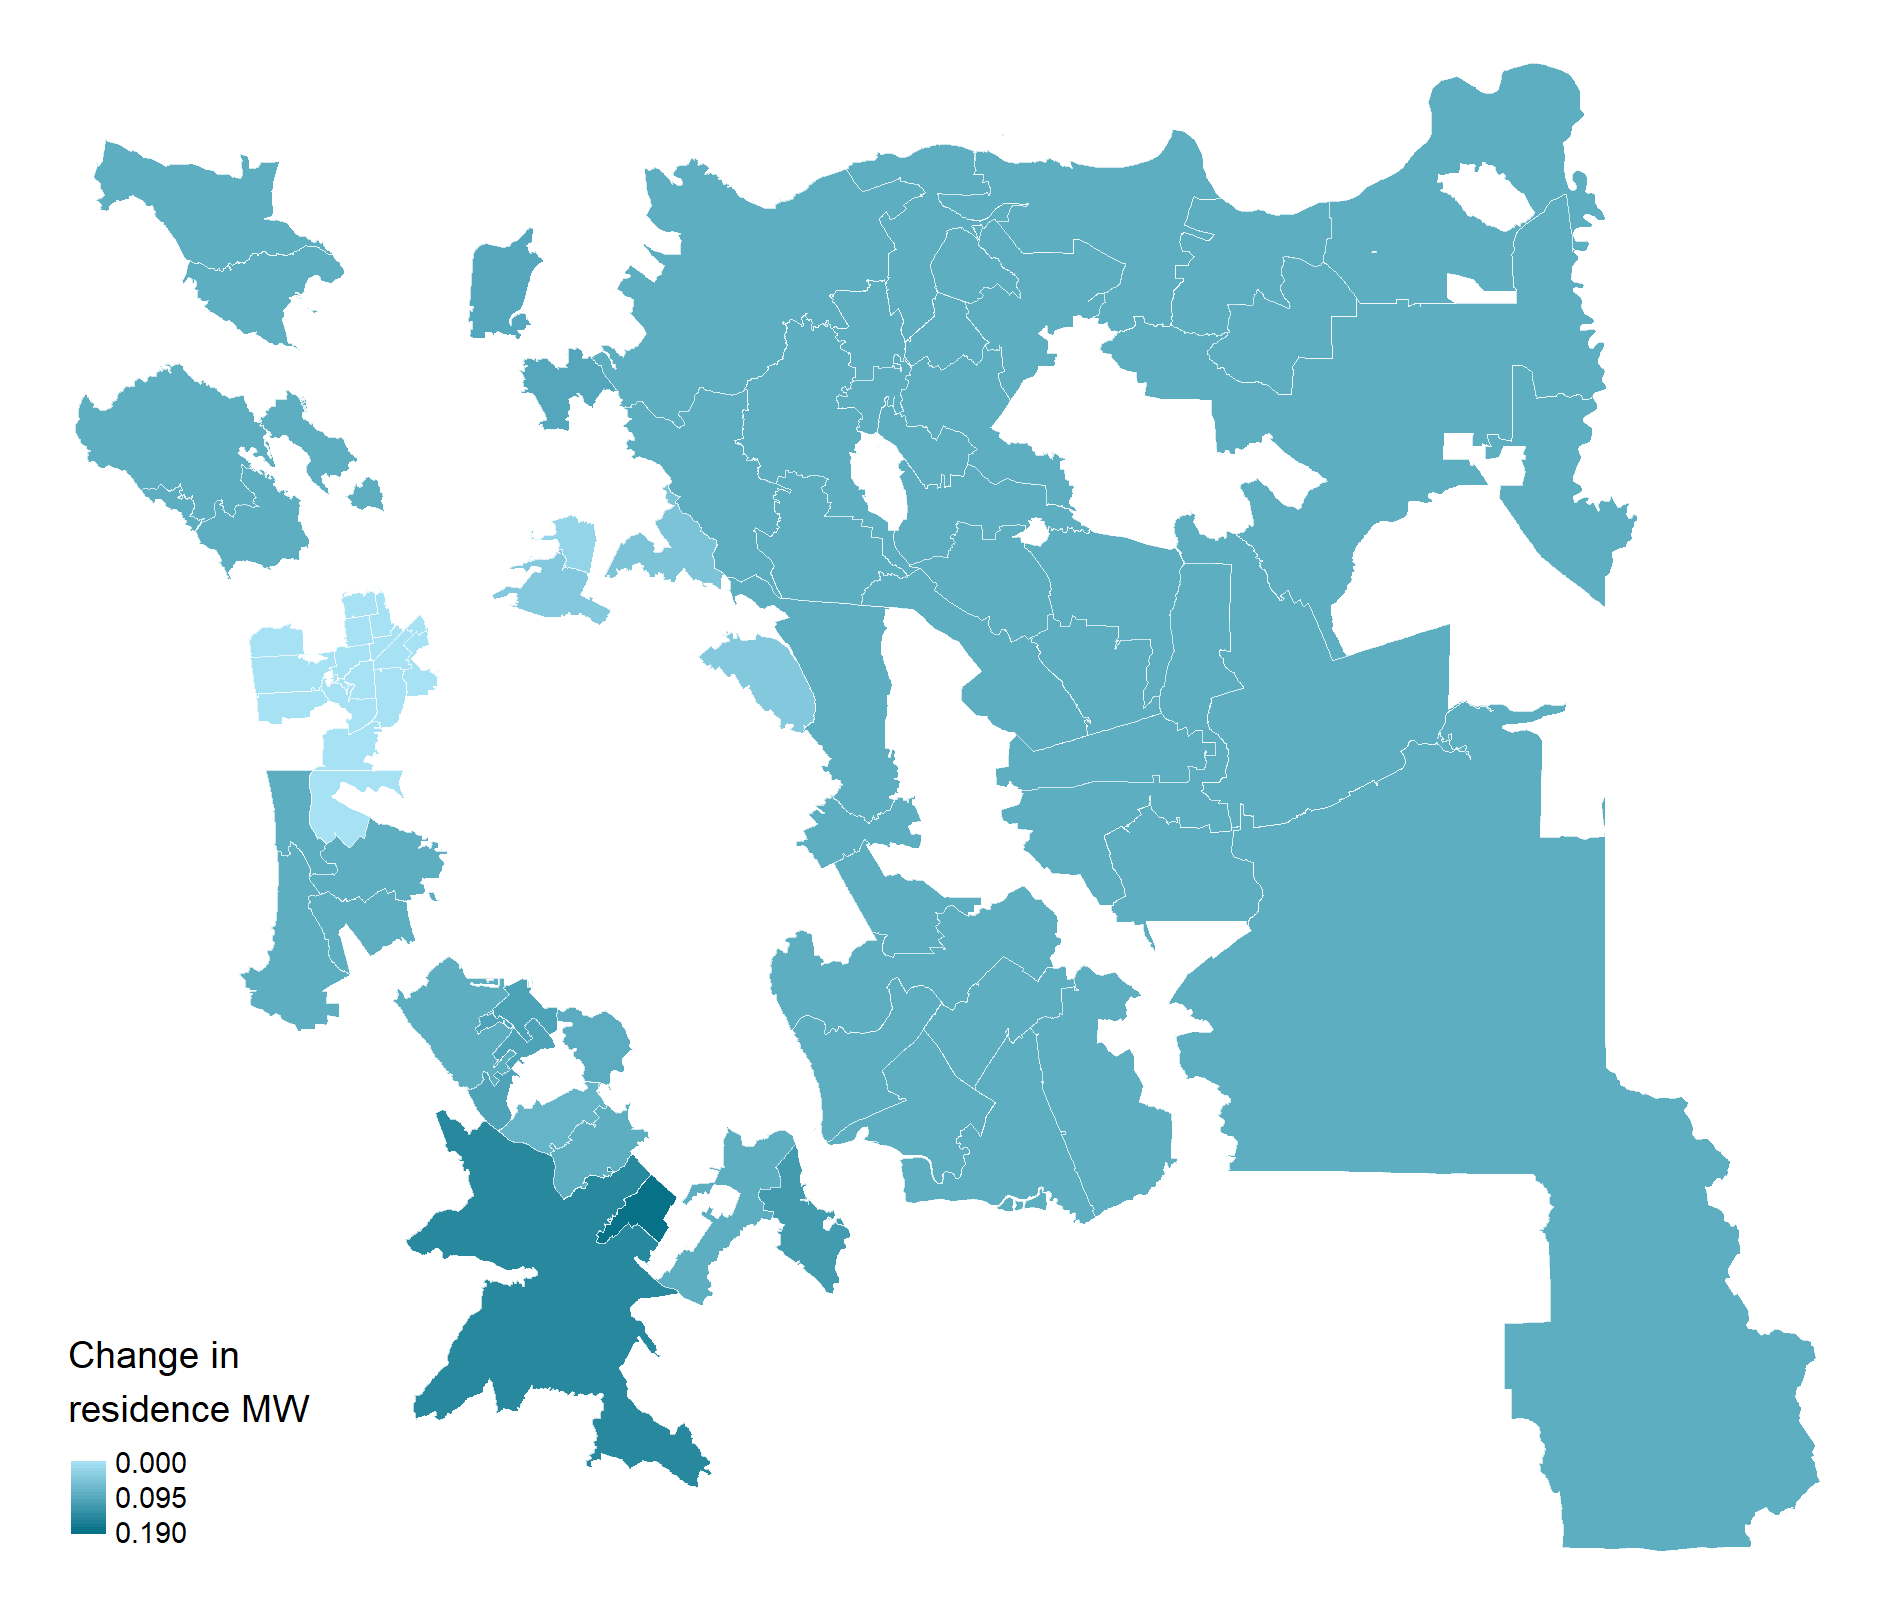
\includegraphics[scale = 0.36]{maps_events/output/bay_area_2018-12_statutory_mw.png}
            \end{figure}   
        \end{column}
        \begin{column}{0.50\textwidth}
            \vspace{-4mm}
            \begin{figure}
                \centering
                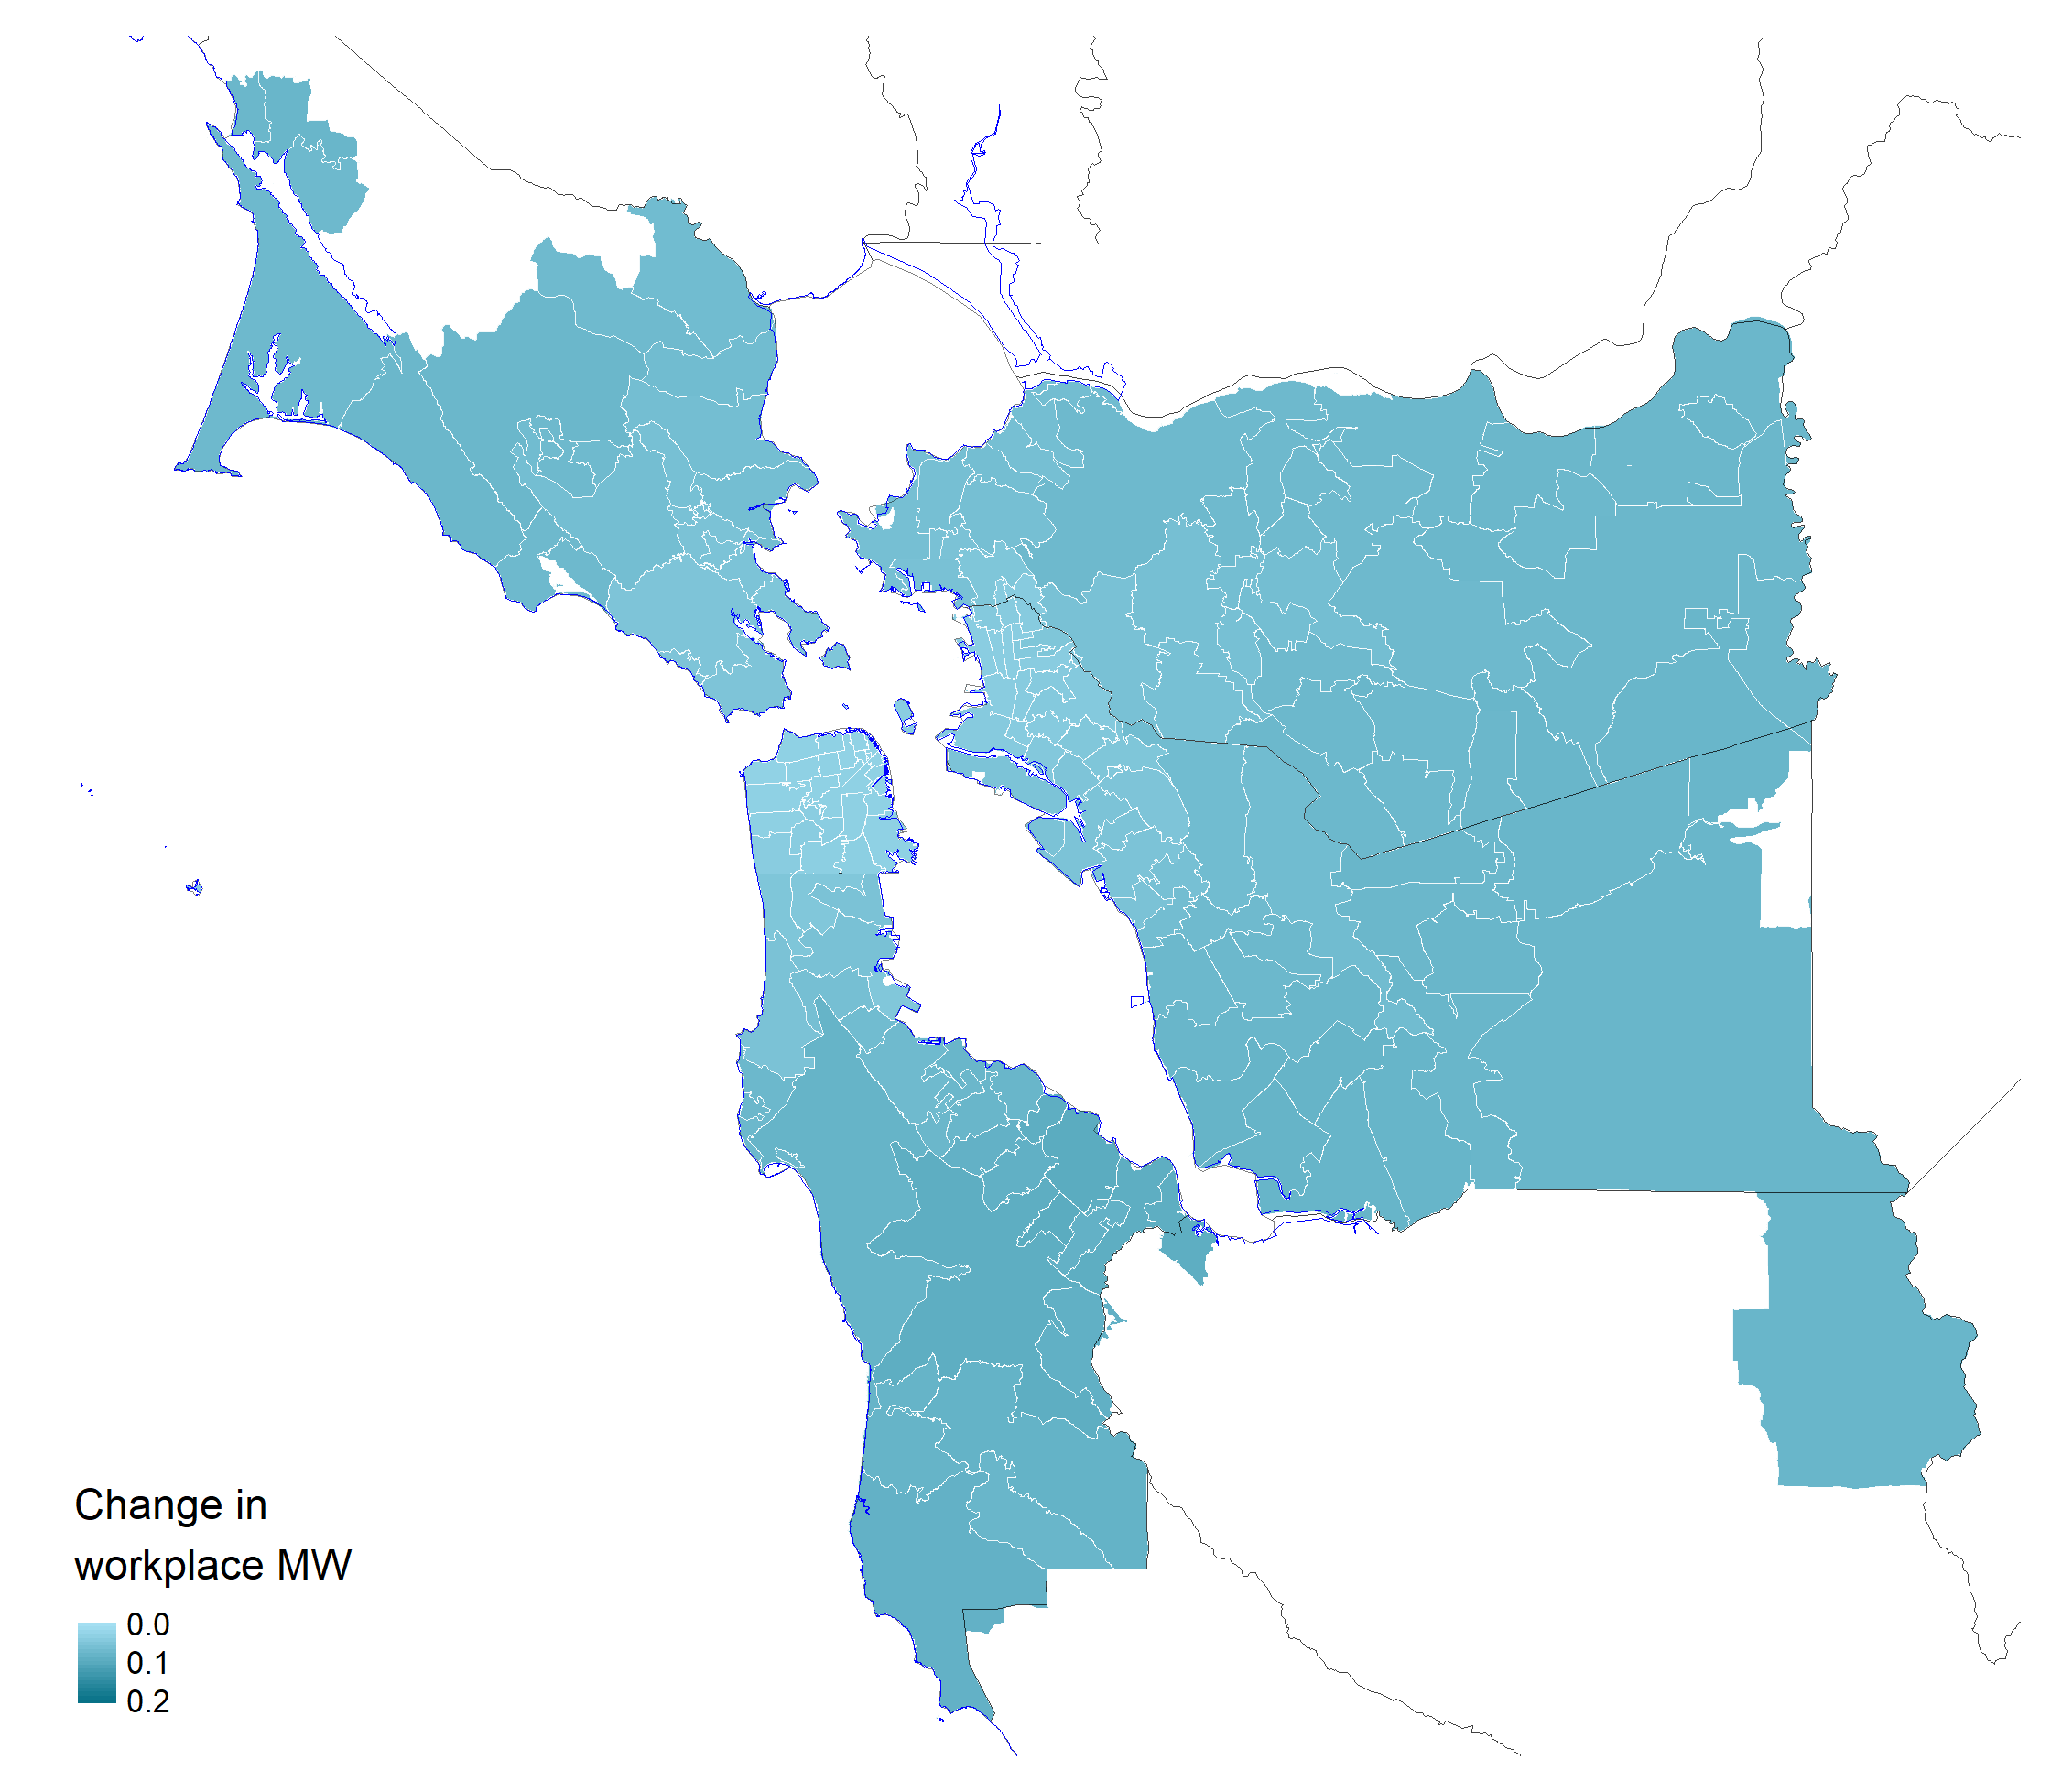
\includegraphics[scale = 0.36]{maps_events/output/bay_area2018-12_wkp_mw.png}
            \end{figure}   
        \end{column}
    \end{columns}
    \hyperlink{chi_example}{\beamerbutton{Go back}}
\end{frame}


\begin{frame}[label = san_diego_example]
\frametitle{San Diego (MW changes in January 2019)}
    \begin{columns}
        \begin{column}{0.50\textwidth}
            \vspace{-4mm}
            \begin{figure}
                \centering
                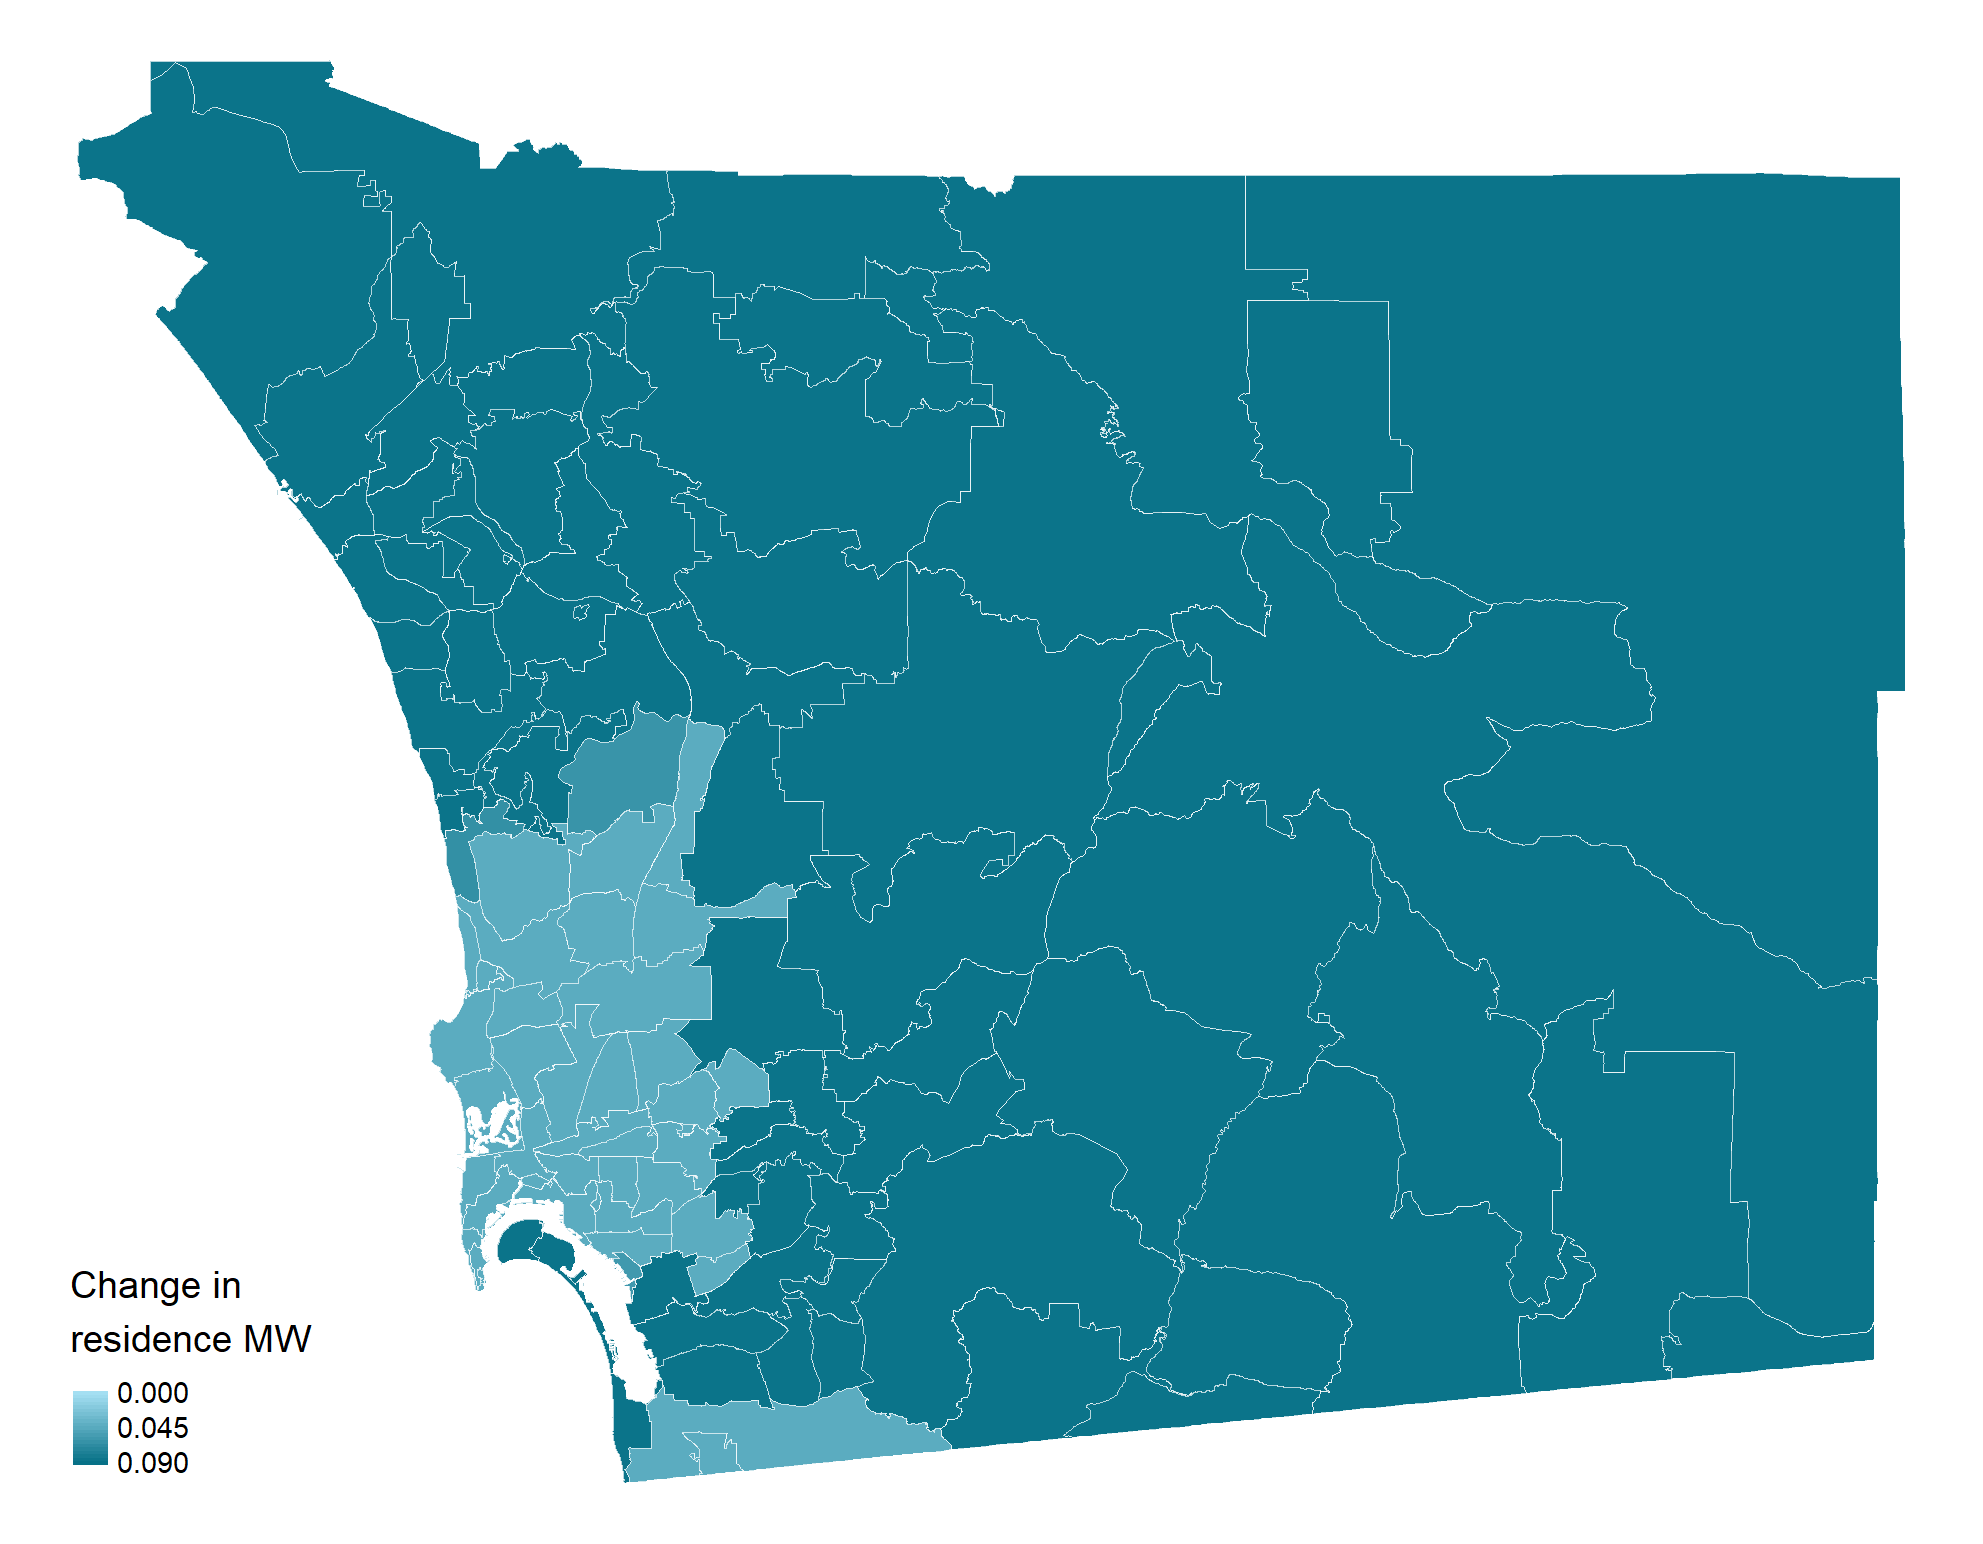
\includegraphics[scale = 0.36]{maps_events/output/san_diego_2018-12_statutory_mw.png}
            \end{figure}   
        \end{column}
        \begin{column}{0.50\textwidth}
            \vspace{-4mm}
            \begin{figure}
                \centering
                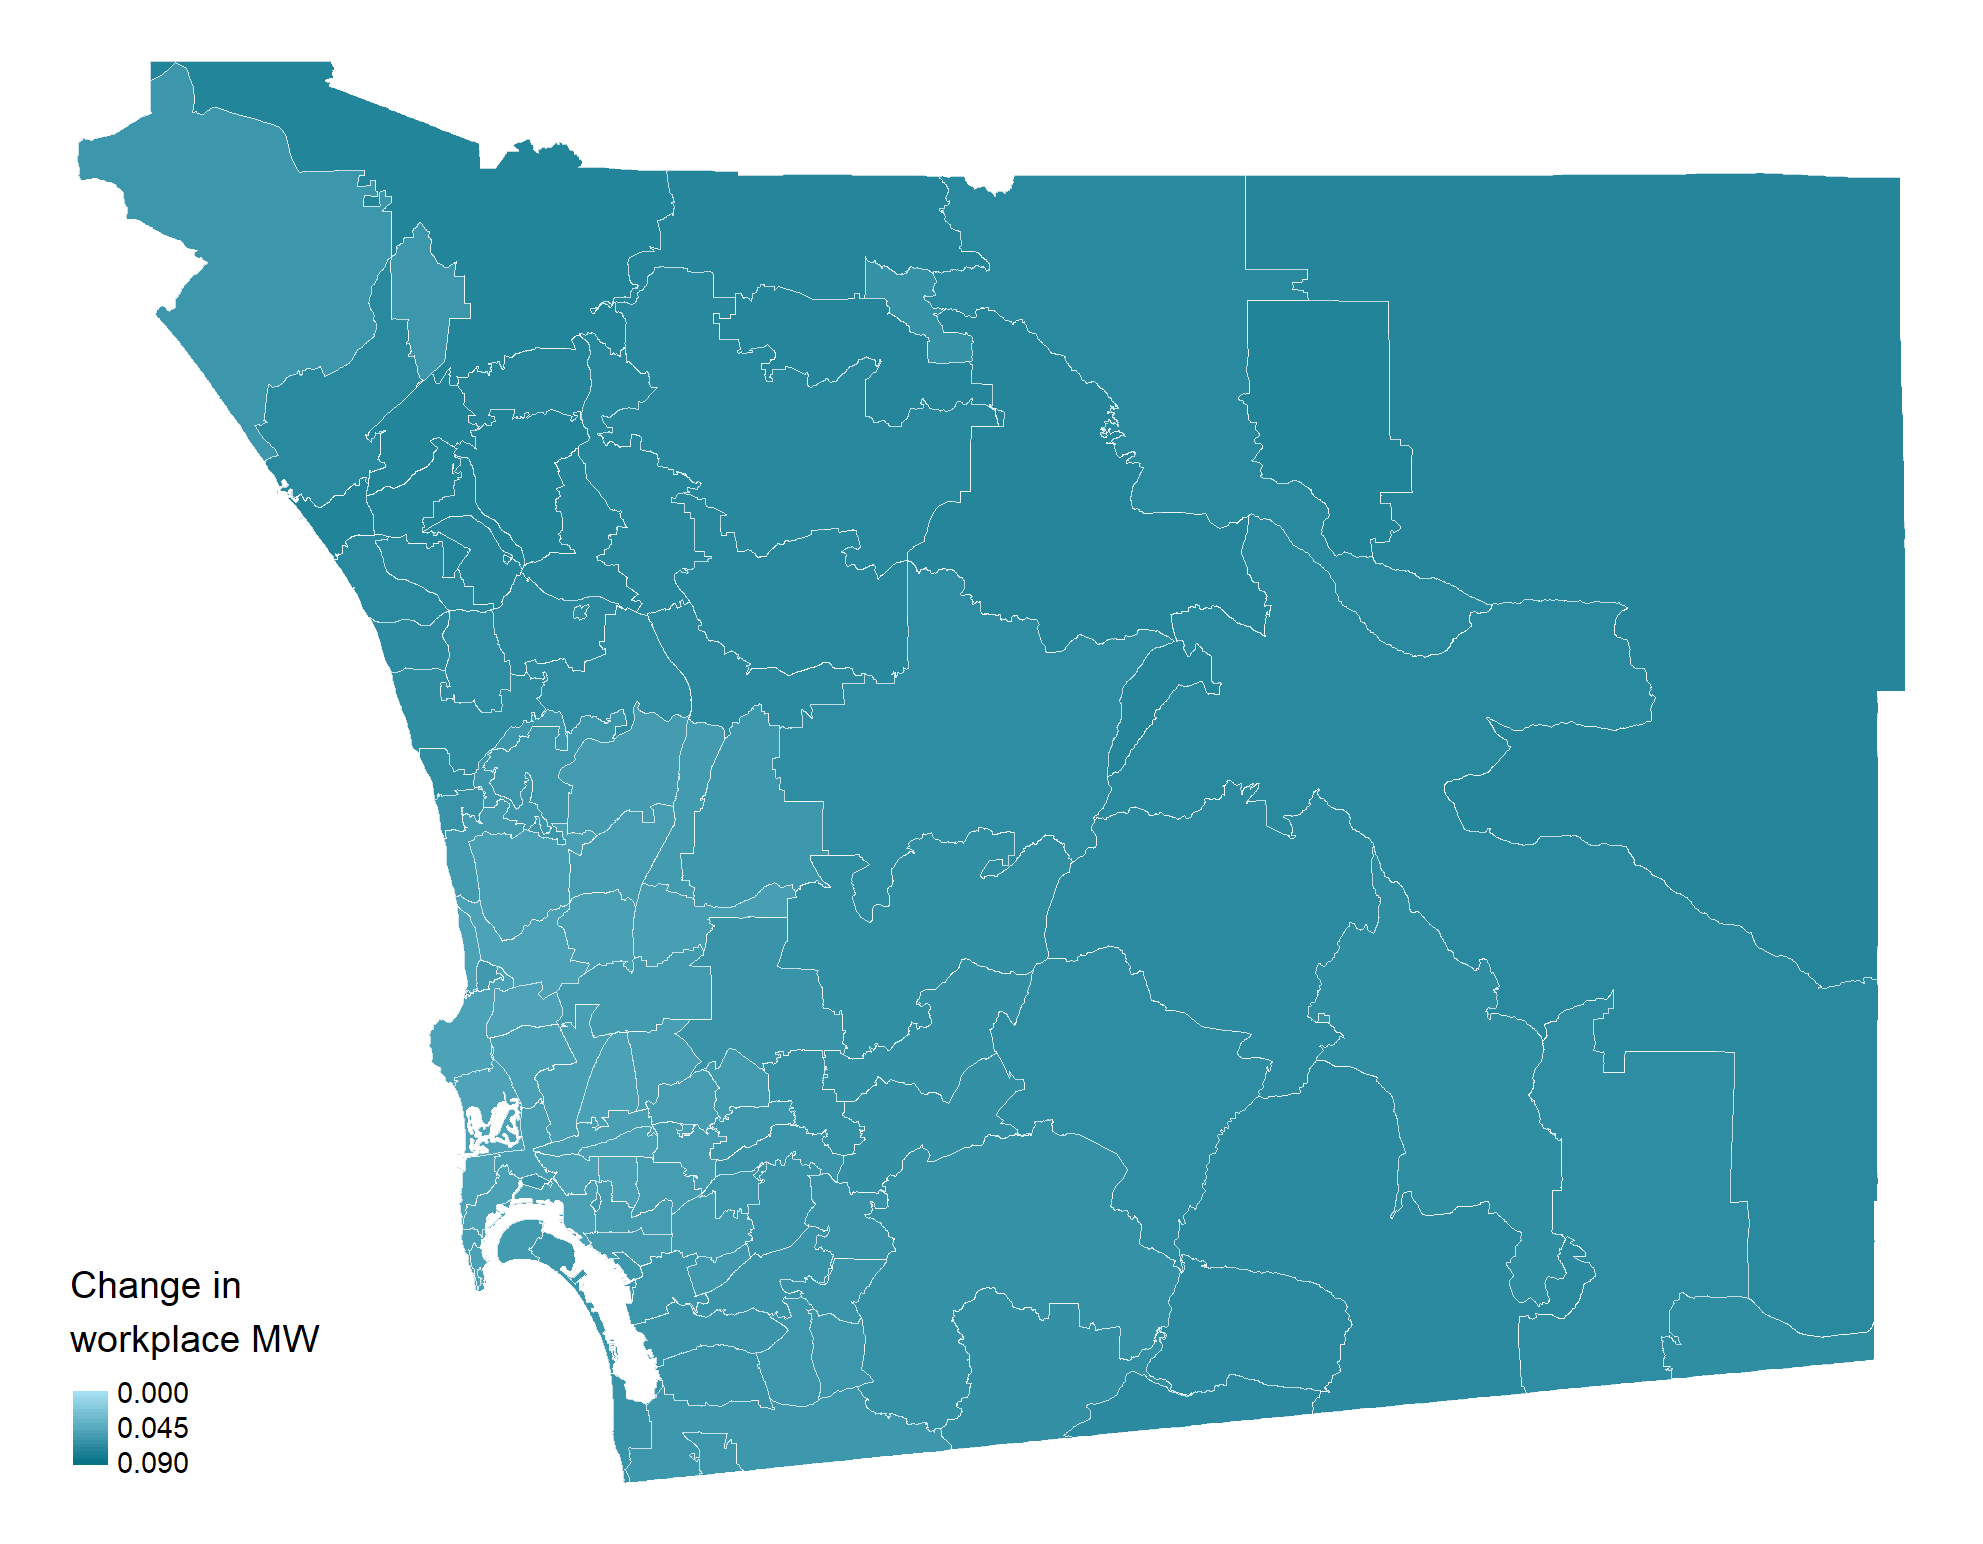
\includegraphics[scale = 0.36]{maps_events/output/san_diego2018-12_wkp_mw.png}
            \end{figure}   
        \end{column}
    \end{columns}
     \hyperlink{chi_example}{\beamerbutton{Go back}}
\end{frame}

\begin{frame}[label = kc_example]
\frametitle{Kansas City (MW changes in January 2019)}
    \begin{columns}
        \begin{column}{0.50\textwidth}
            \vspace{-4mm}
            \begin{figure}
                \centering
                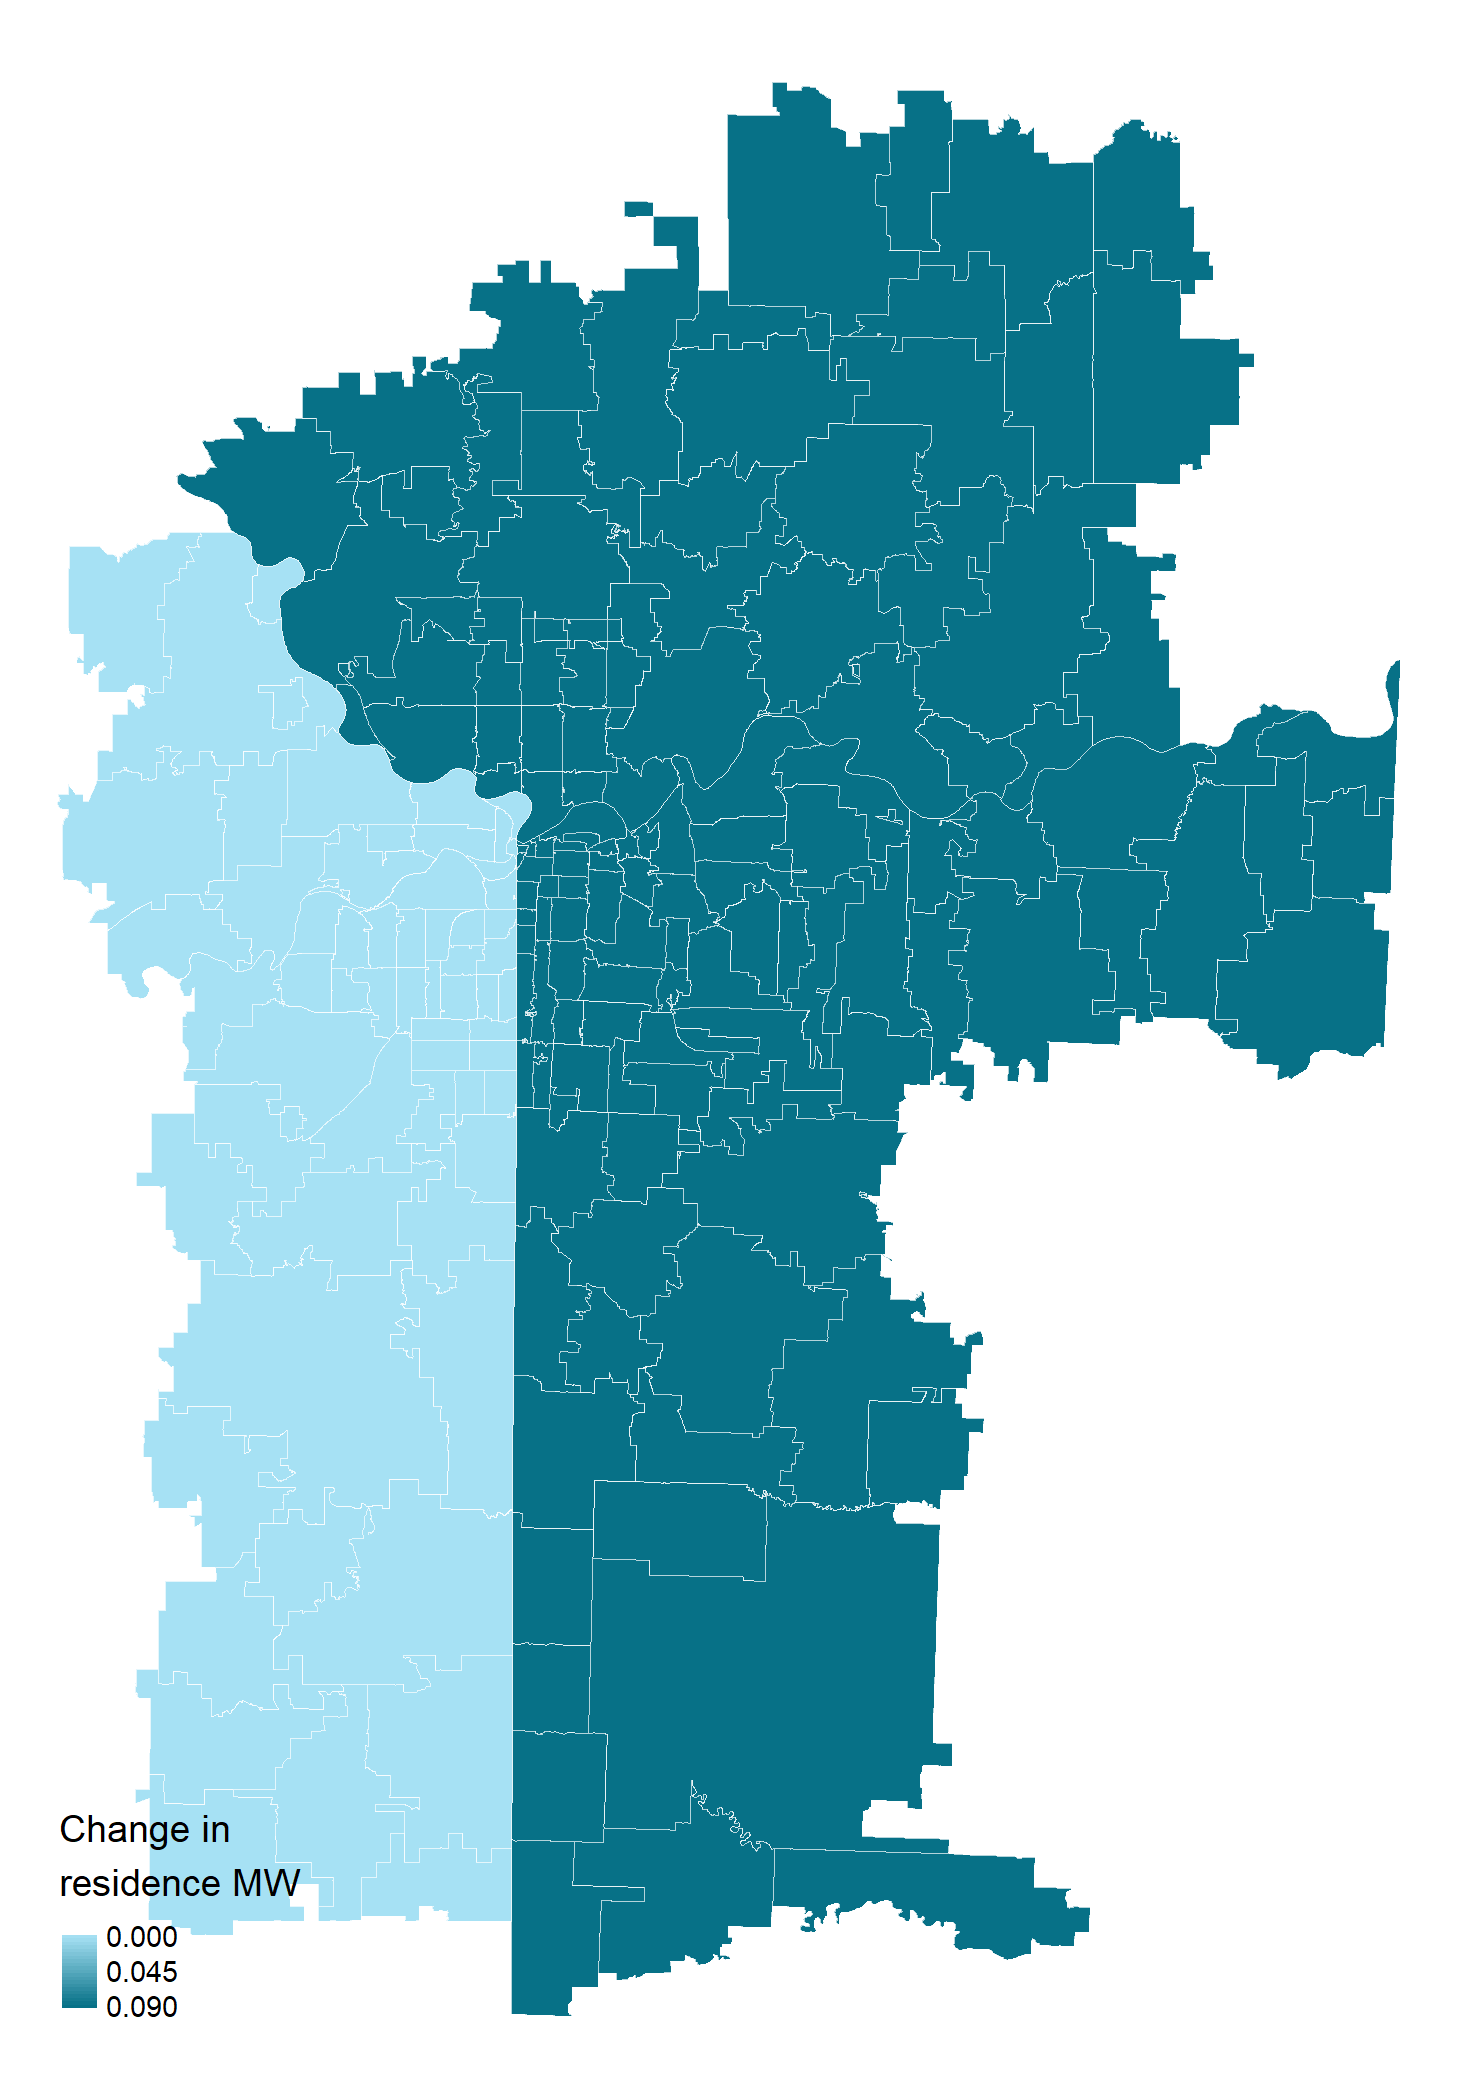
\includegraphics[scale = 0.36]{maps_events/output/kc_2018-12_statutory_mw.png}
            \end{figure}   
        \end{column}
        \begin{column}{0.50\textwidth}
            \vspace{-4mm}
            \begin{figure}
                \centering
                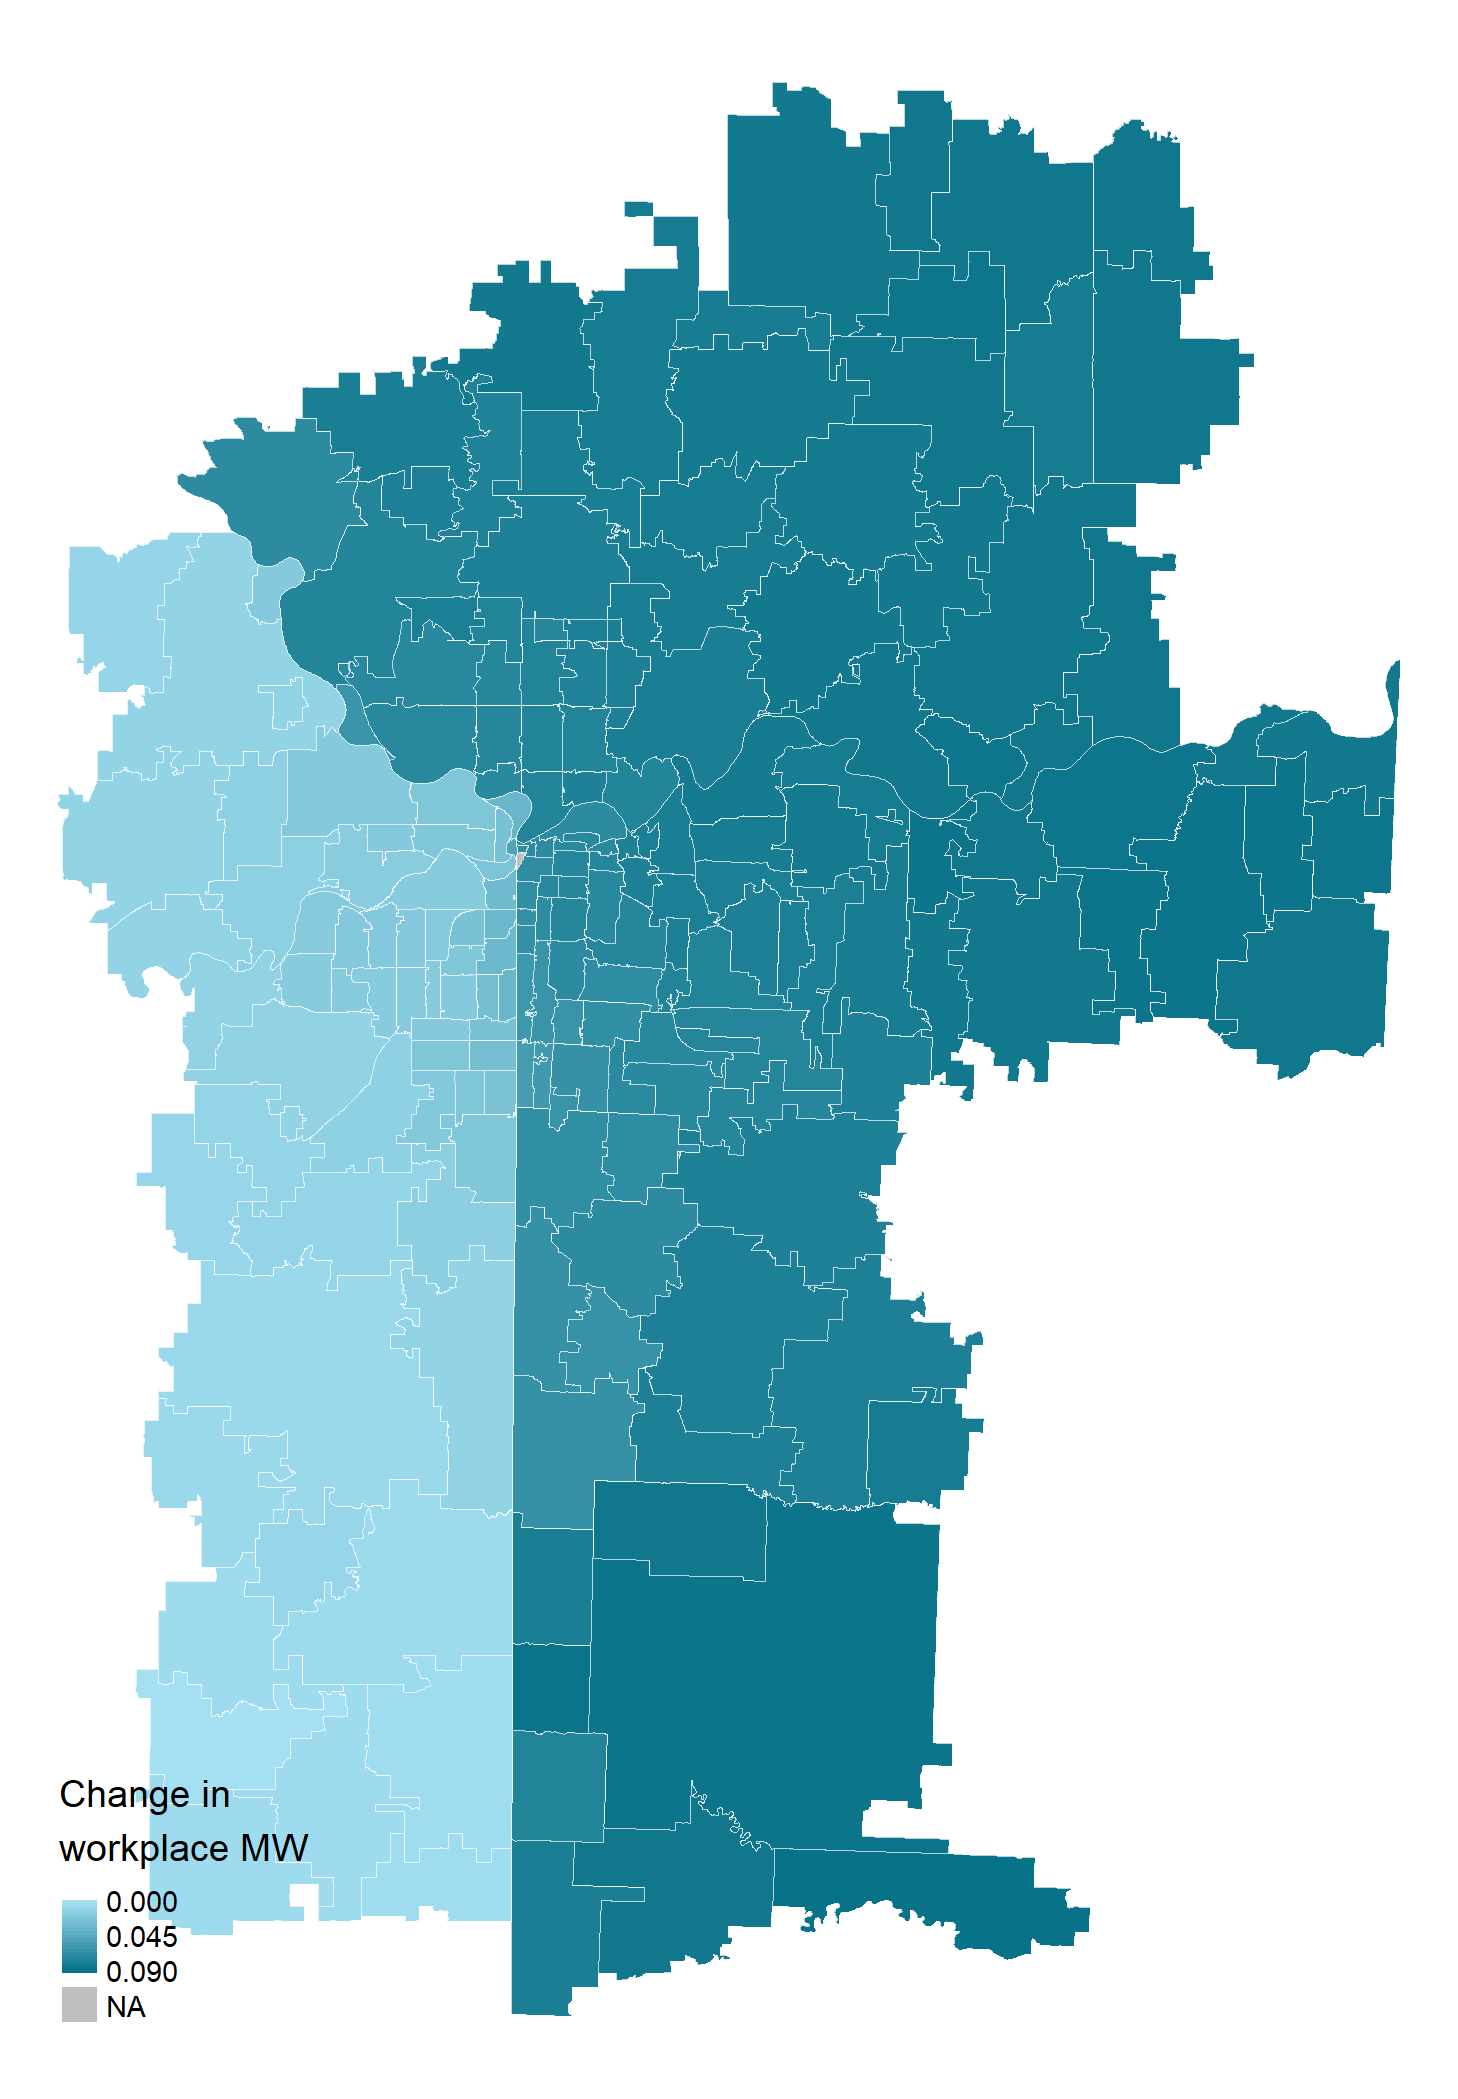
\includegraphics[scale = 0.36]{maps_events/output/kc2018-12_wkp_mw.png}
            \end{figure}   
        \end{column}
    \end{columns}
     \hyperlink{chi_example}{\beamerbutton{Go back}}
\end{frame}

\begin{frame}[label = microfound]
    \frametitle{Microfoundation}
    Say a representative $(i,z)$ worker chooses between housing demand $h_{iz}$,
    non-tradable consumption $c^{\text{NT}}_{iz}$, and tradable consumption $c^{\text{T}}_{iz}$,
    by maximizing
    \[
    u_{iz} = u \left(h_{iz}, c^{\text{NT}}_{iz}, c^{\text{T}}_{iz}\right)
    \]
    subject to

    \[
    r_i h_{iz} + p_i(\MW_i) c^{\text{NT}}_{iz} + c^{\text{T}}_{iz} \leq y_{iz}(\MW_z)
    \]

    where 
    \begin{itemize}
        \item $p_i(\MW_i)$ gives the price of local consumption, increasing in residence MW;
        \item the price of tradable consumption is normalized to one;  
        \item $y_{iz}(\MW_z)$ is an income function that depends positively on the workplace MW.
    \end{itemize}
\end{frame}

\begin{frame}[label = zillow_pop_density]
    \frametitle{Comparison between Zillow Sample and Population Density}
    \begin{figure}
        \centering
    \vspace{10mm}
    \hspace{-23mm}
        \begin{subfigure}{0.40\textwidth}
            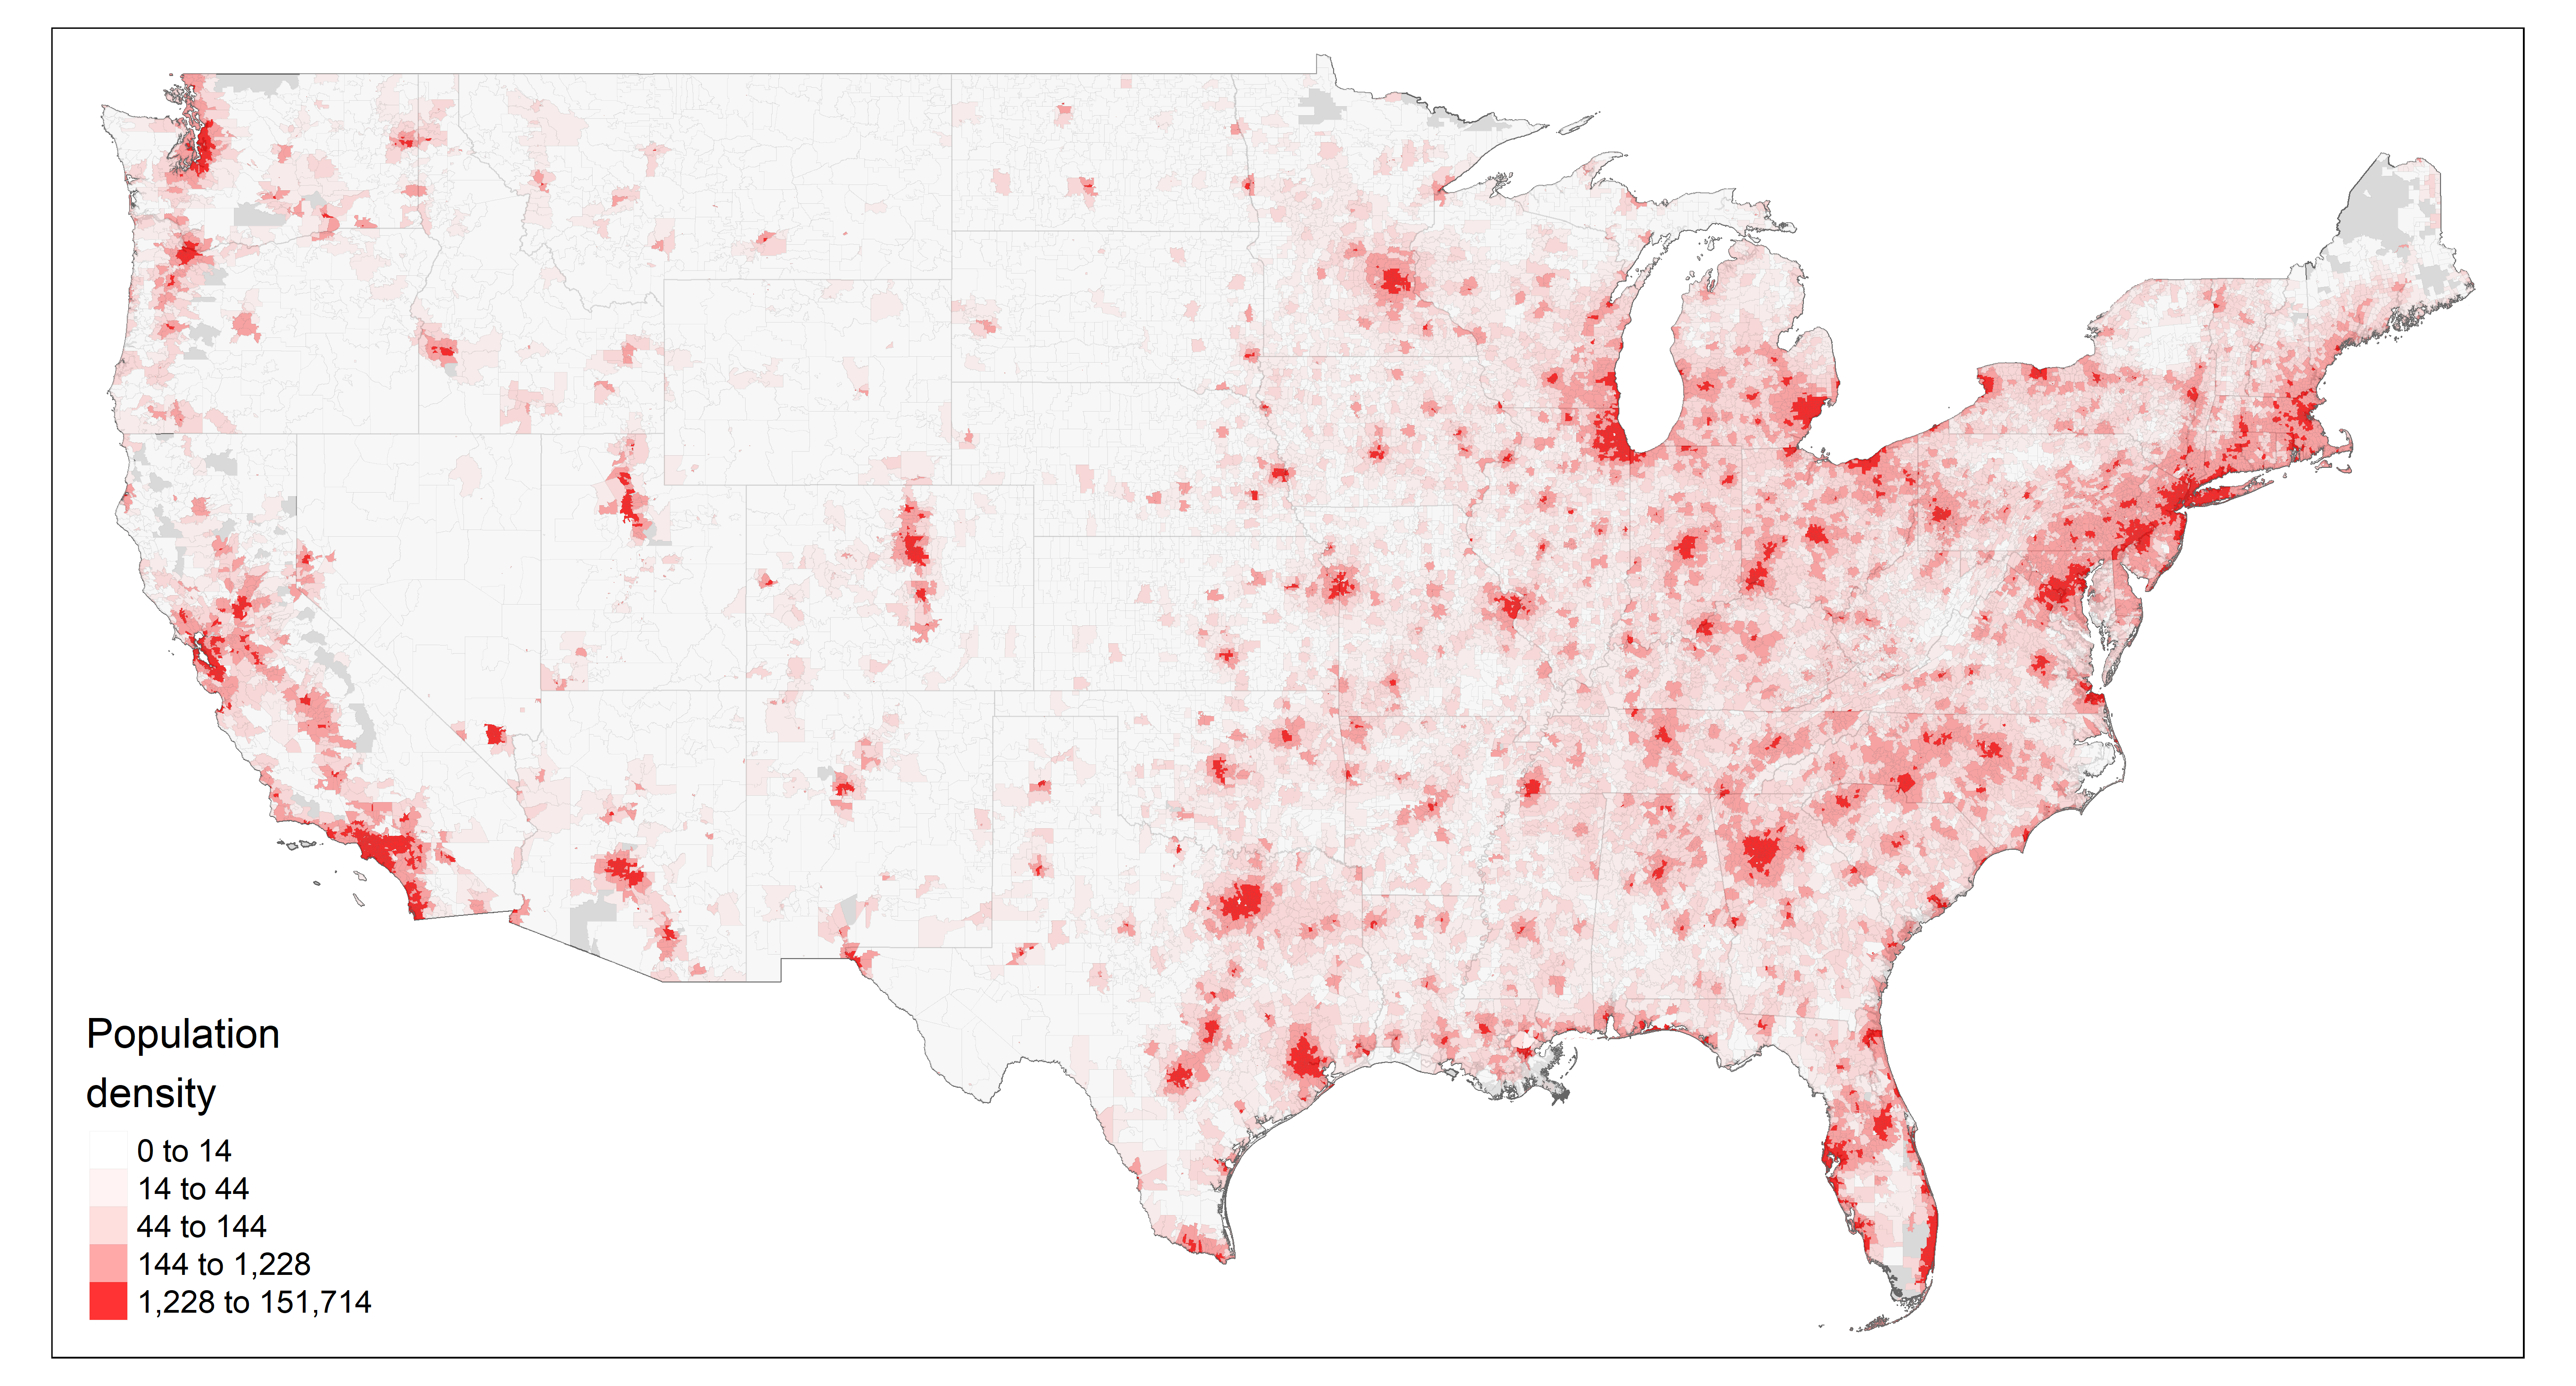
\includegraphics[scale = 0.32]{maps_US/output/USPS_zipcodes_pop_density.png}
        \end{subfigure}%
    \quad\quad\quad\quad\quad\quad
        \begin{subfigure}{0.40\textwidth}
            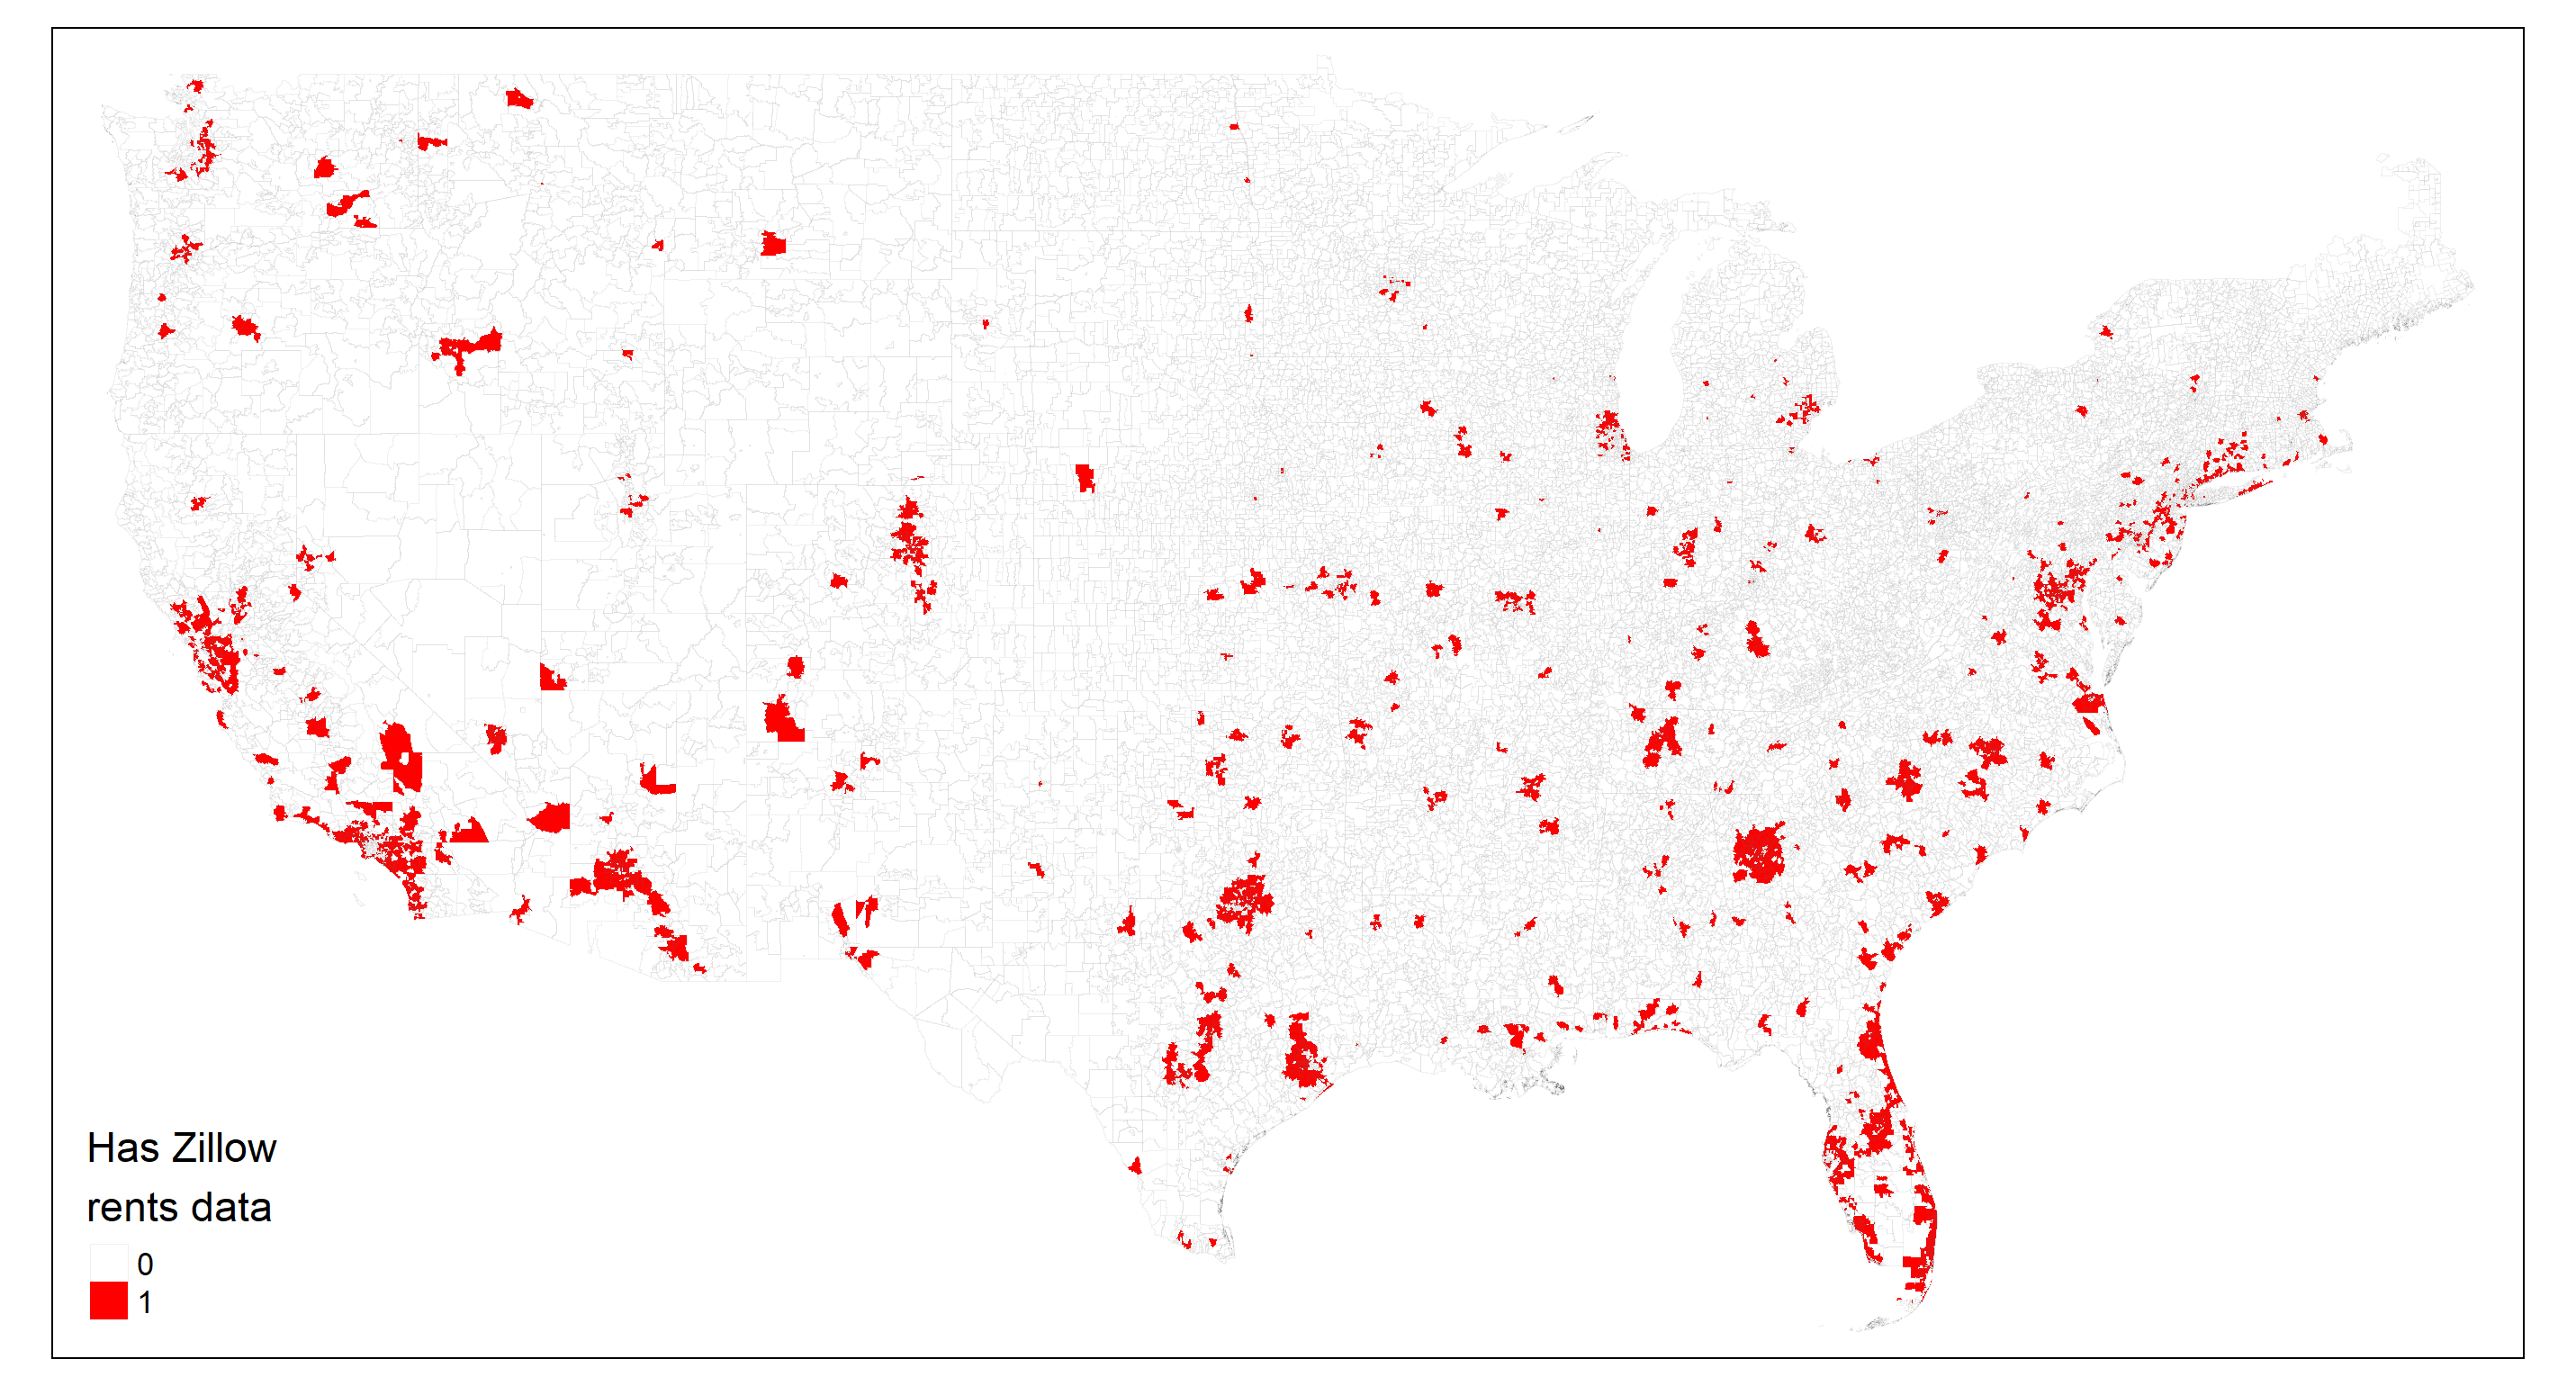
\includegraphics[scale = 0.32]{maps_US/output/USPS_zipcodes_zillow_data.png}
        \end{subfigure}
    \end{figure}
    \hyperlink{zillow_data}{\beamerbutton{Go Back}}
\end{frame}

\begin{frame}[label=dist_mw_changes]
    \frametitle{Distribution of (positive) MW changes}
    \begin{figure}
        \begin{subfigure}{0.49\textwidth}
            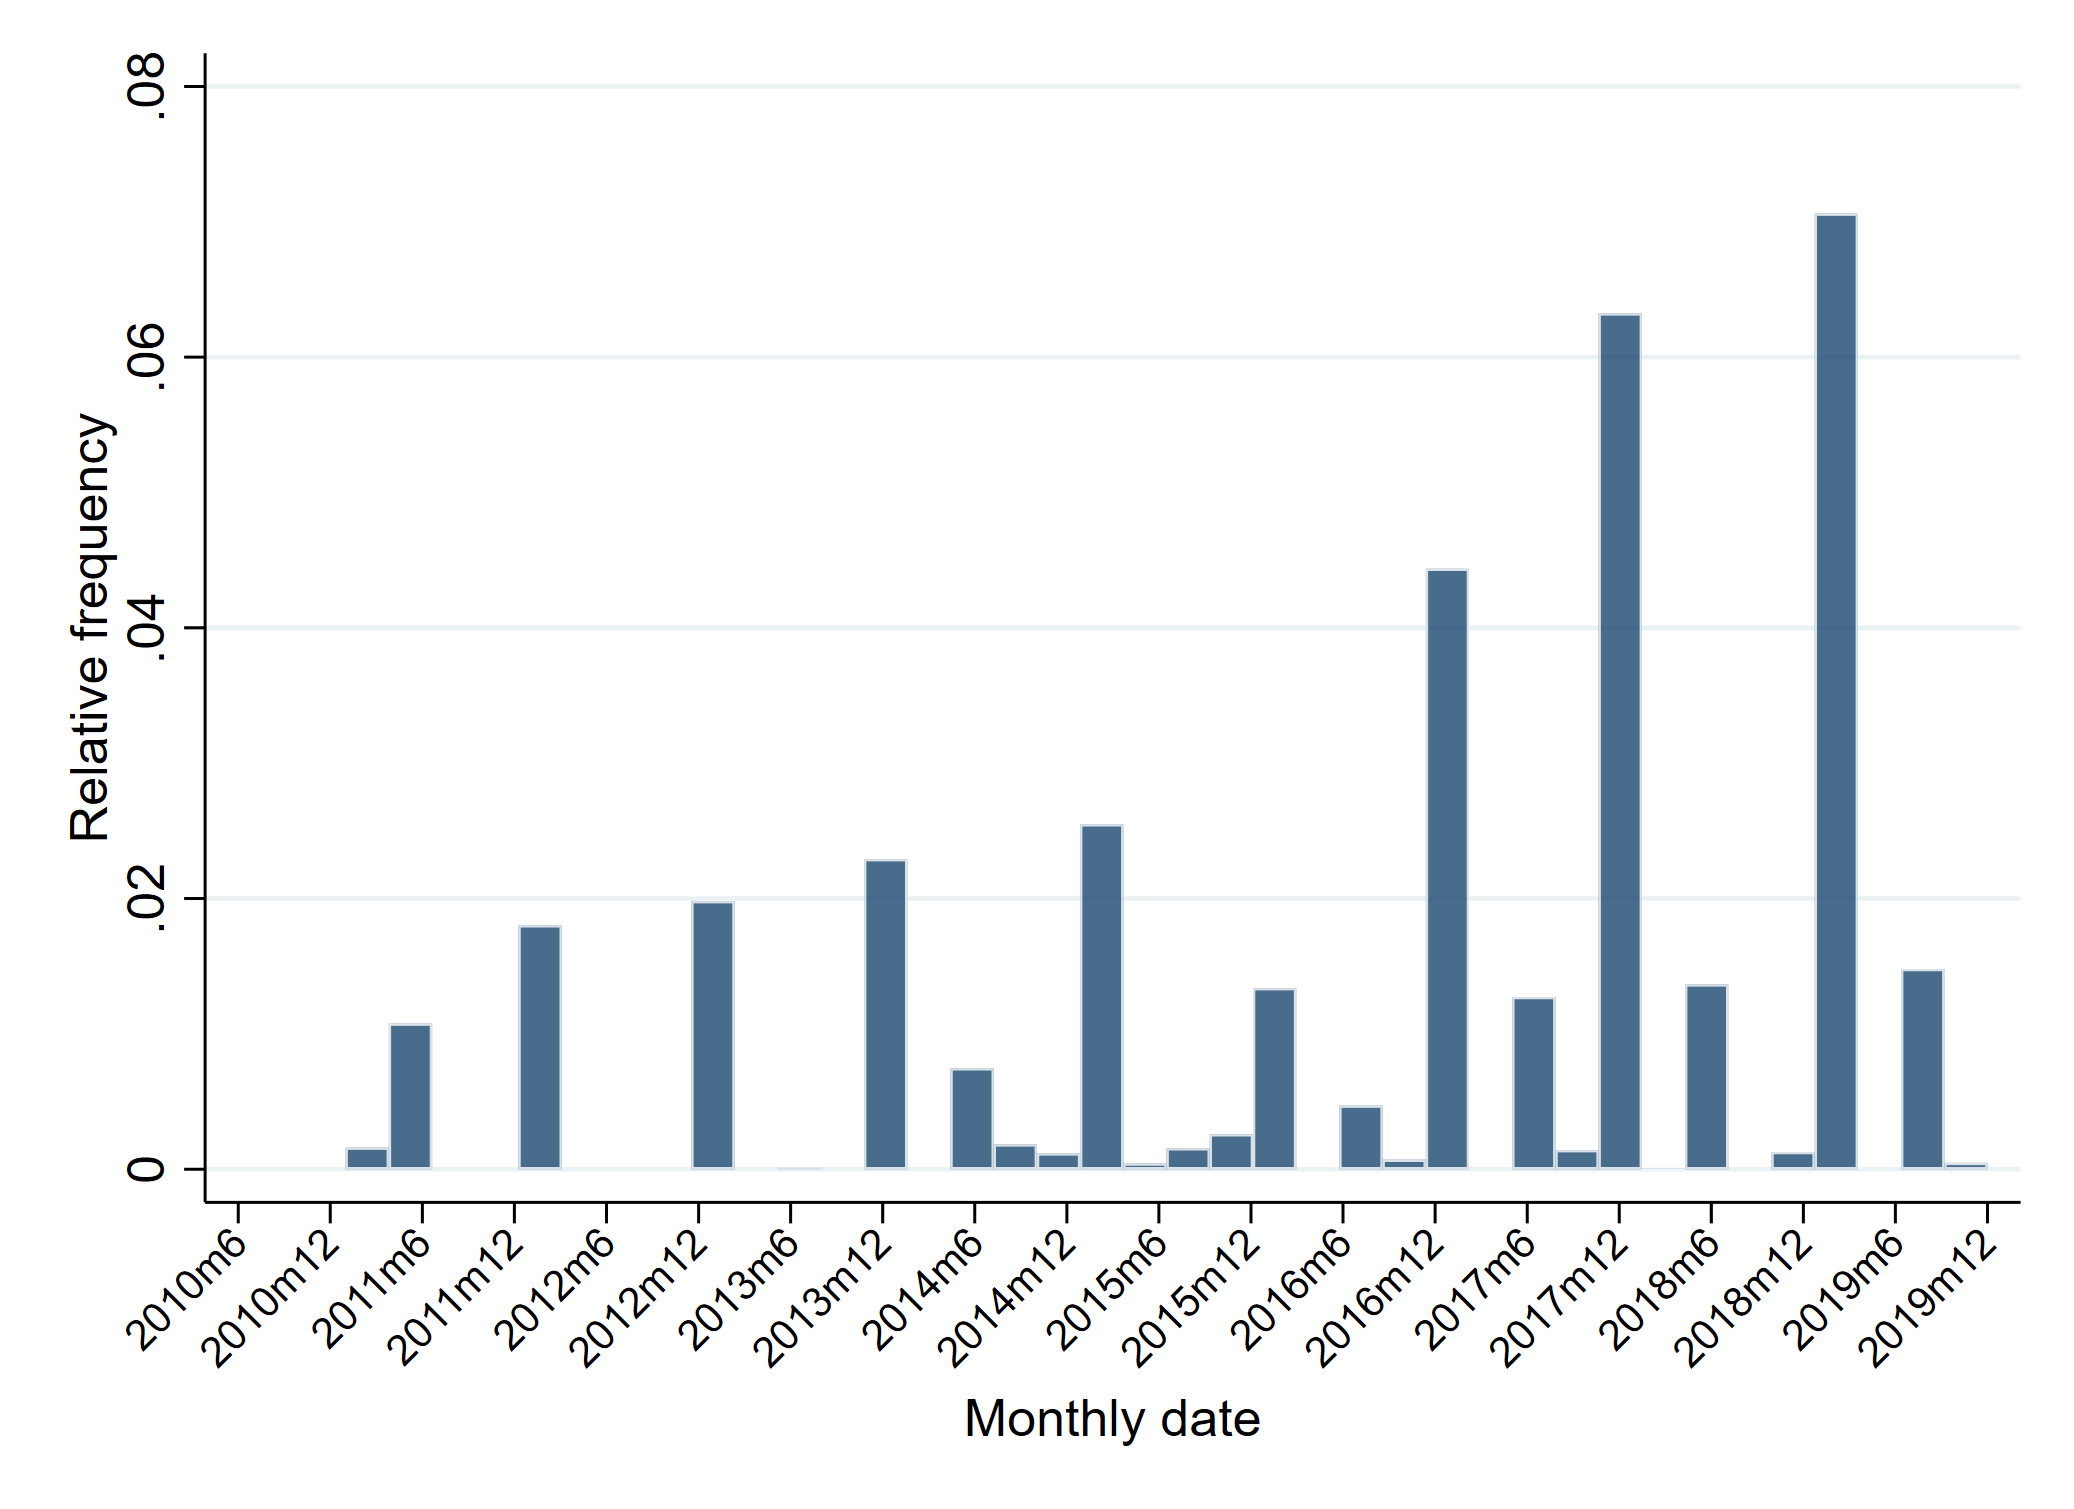
\includegraphics[width = 0.99\textwidth]{estimation_samples/output/pct_ch_mw_date_dist.png}
        \end{subfigure}%
        \begin{subfigure}{0.49\textwidth}
            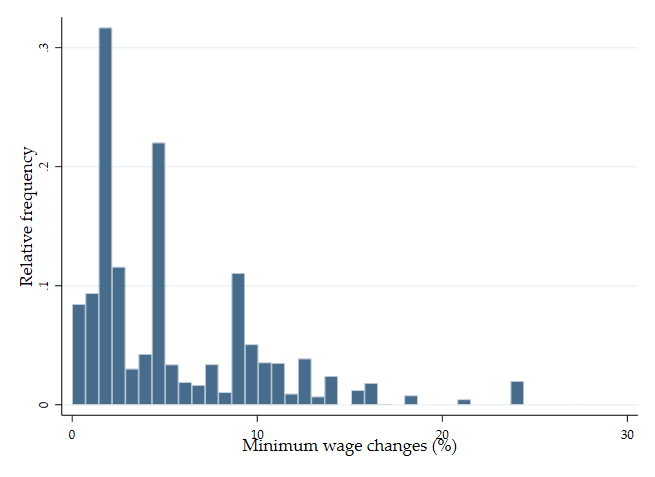
\includegraphics[width = 0.99\textwidth]{estimation_samples/output/pct_ch_mw_dist.png}
        \end{subfigure}
    \end{figure}
    
    \hyperlink{stat_MW}{\beamerbutton{Go Back}}
\end{frame}

\begin{frame}[label = example_pred_chi_07_2019]
    \frametitle{Example Predictions: MMW change in Chicago July 2019}
    
    \begin{figure}
        \begin{subfigure}{0.33\textwidth}
            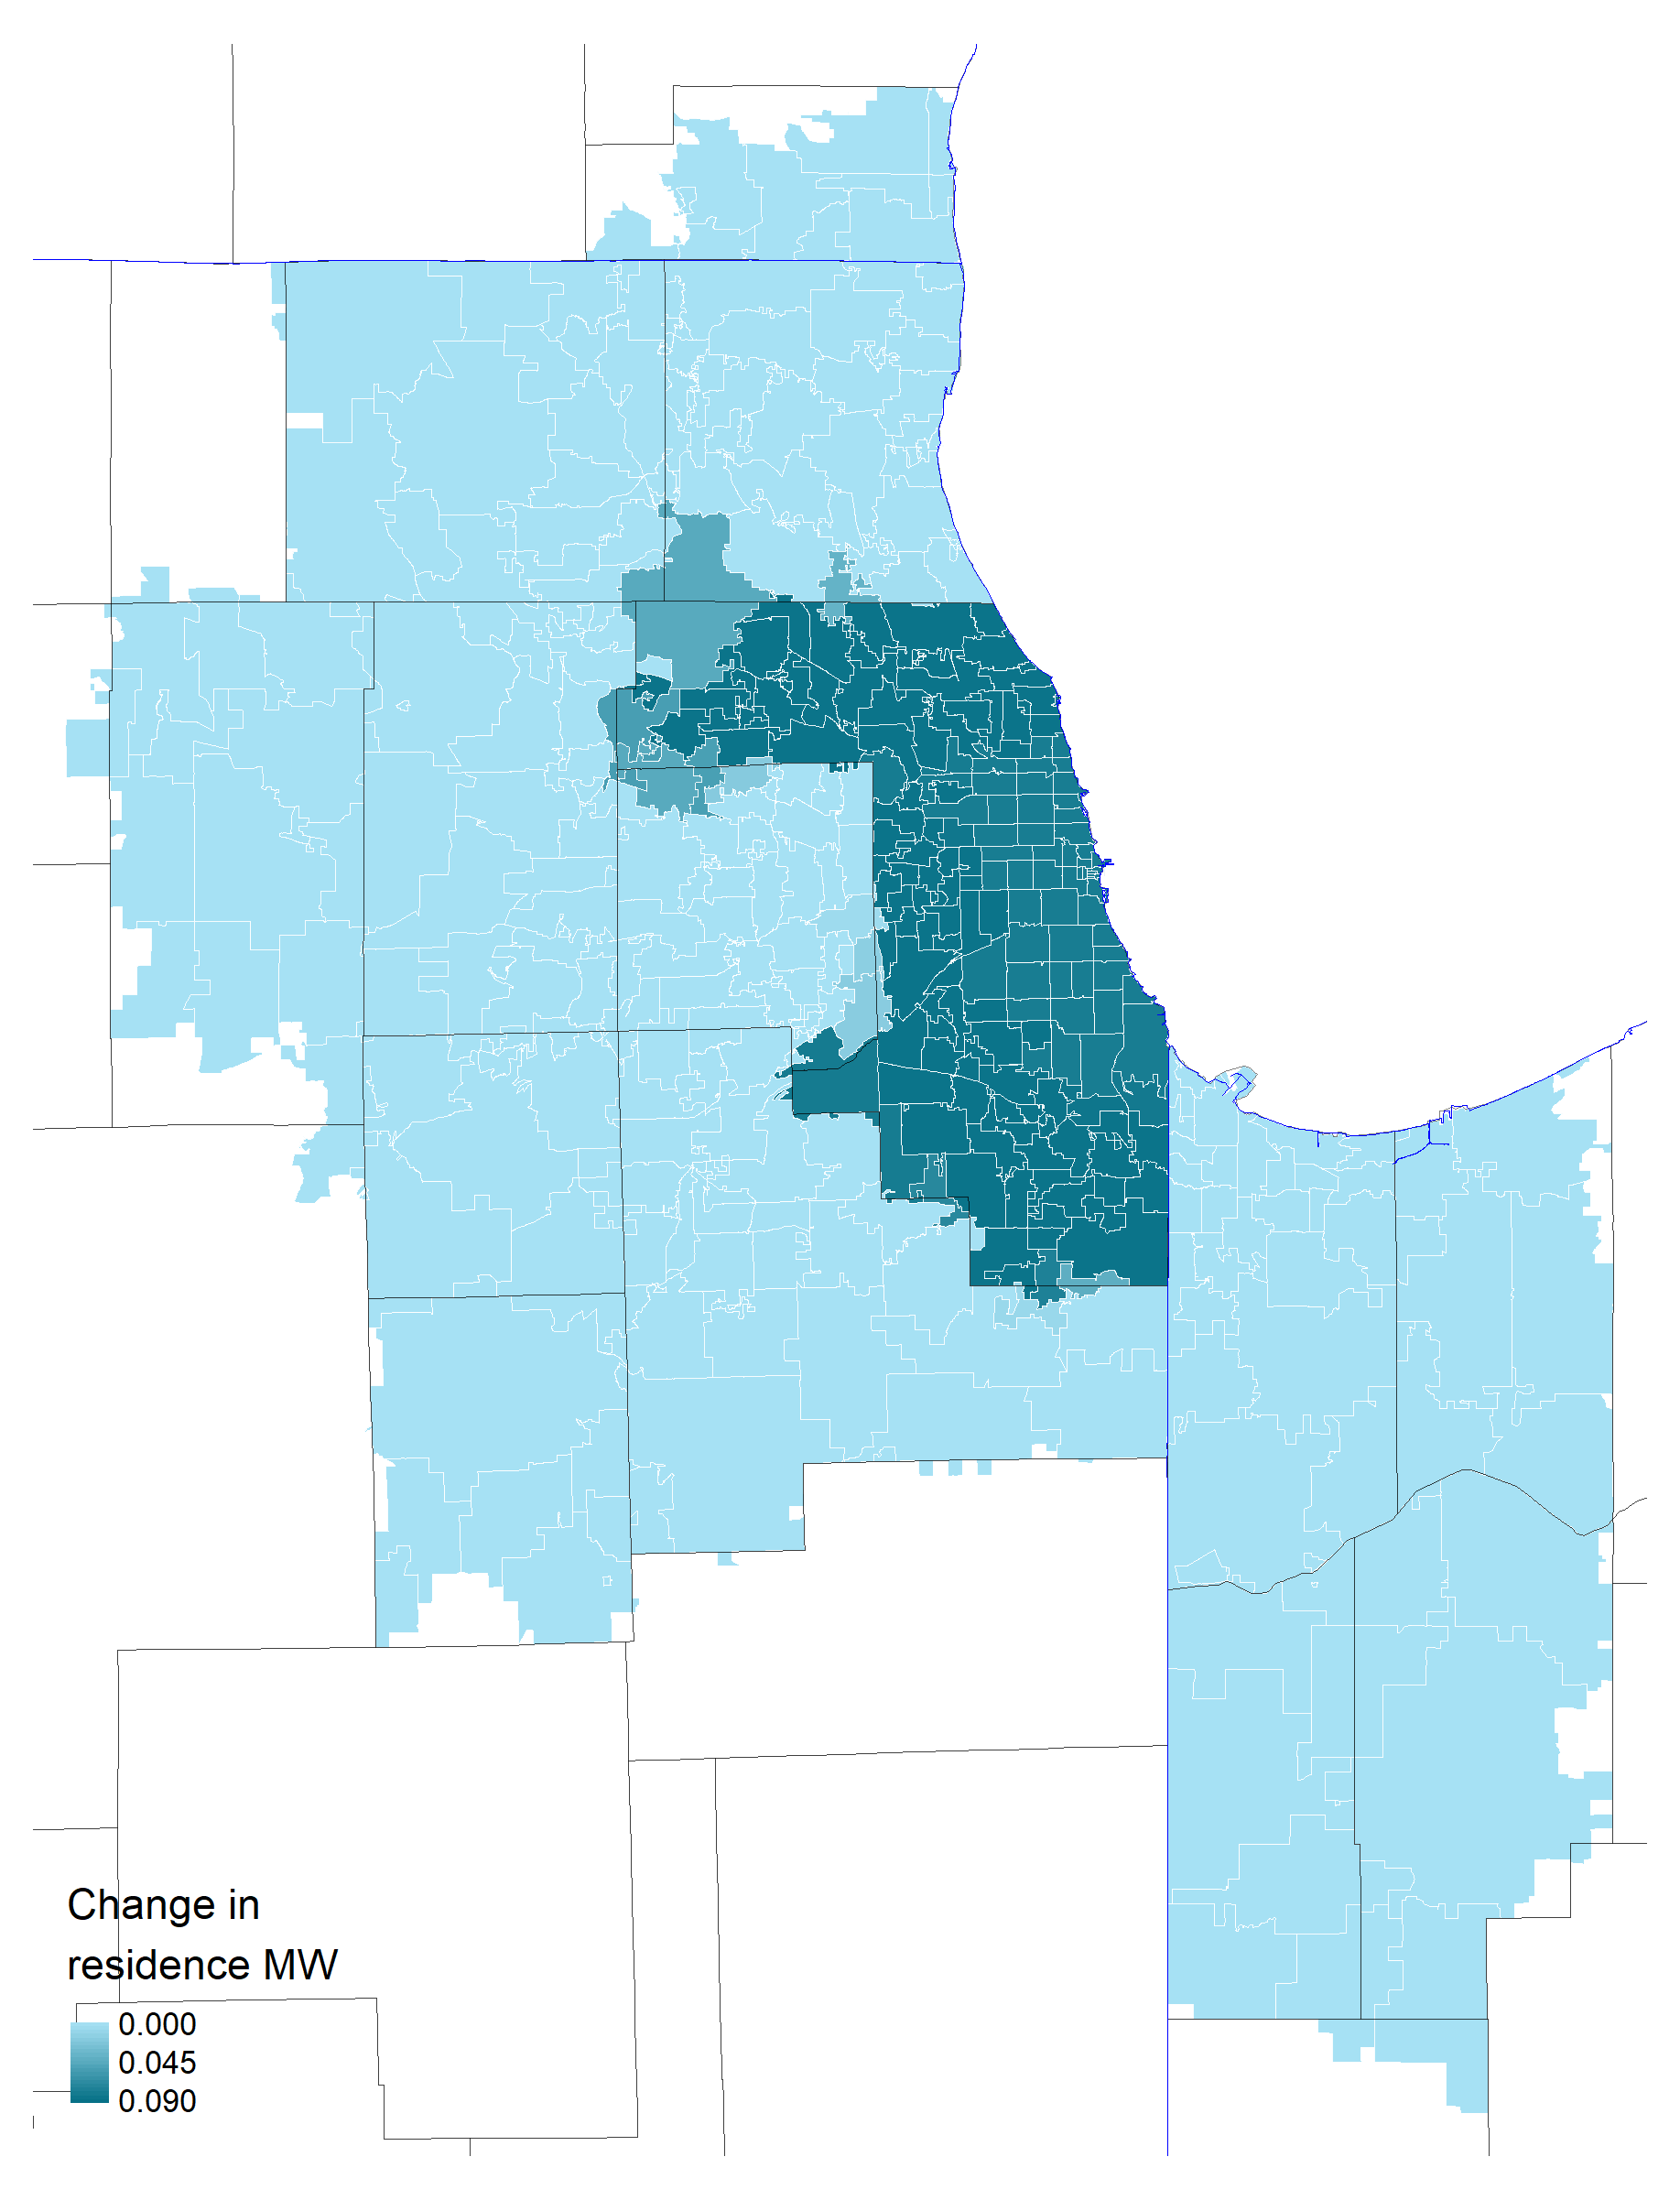
\includegraphics[width = 0.99\textwidth]{maps_events/output/chicago_2019-6_statutory_mw.png}
            \caption*{Change in residence MW}
        \end{subfigure}%
        \begin{subfigure}{0.33\textwidth}
                         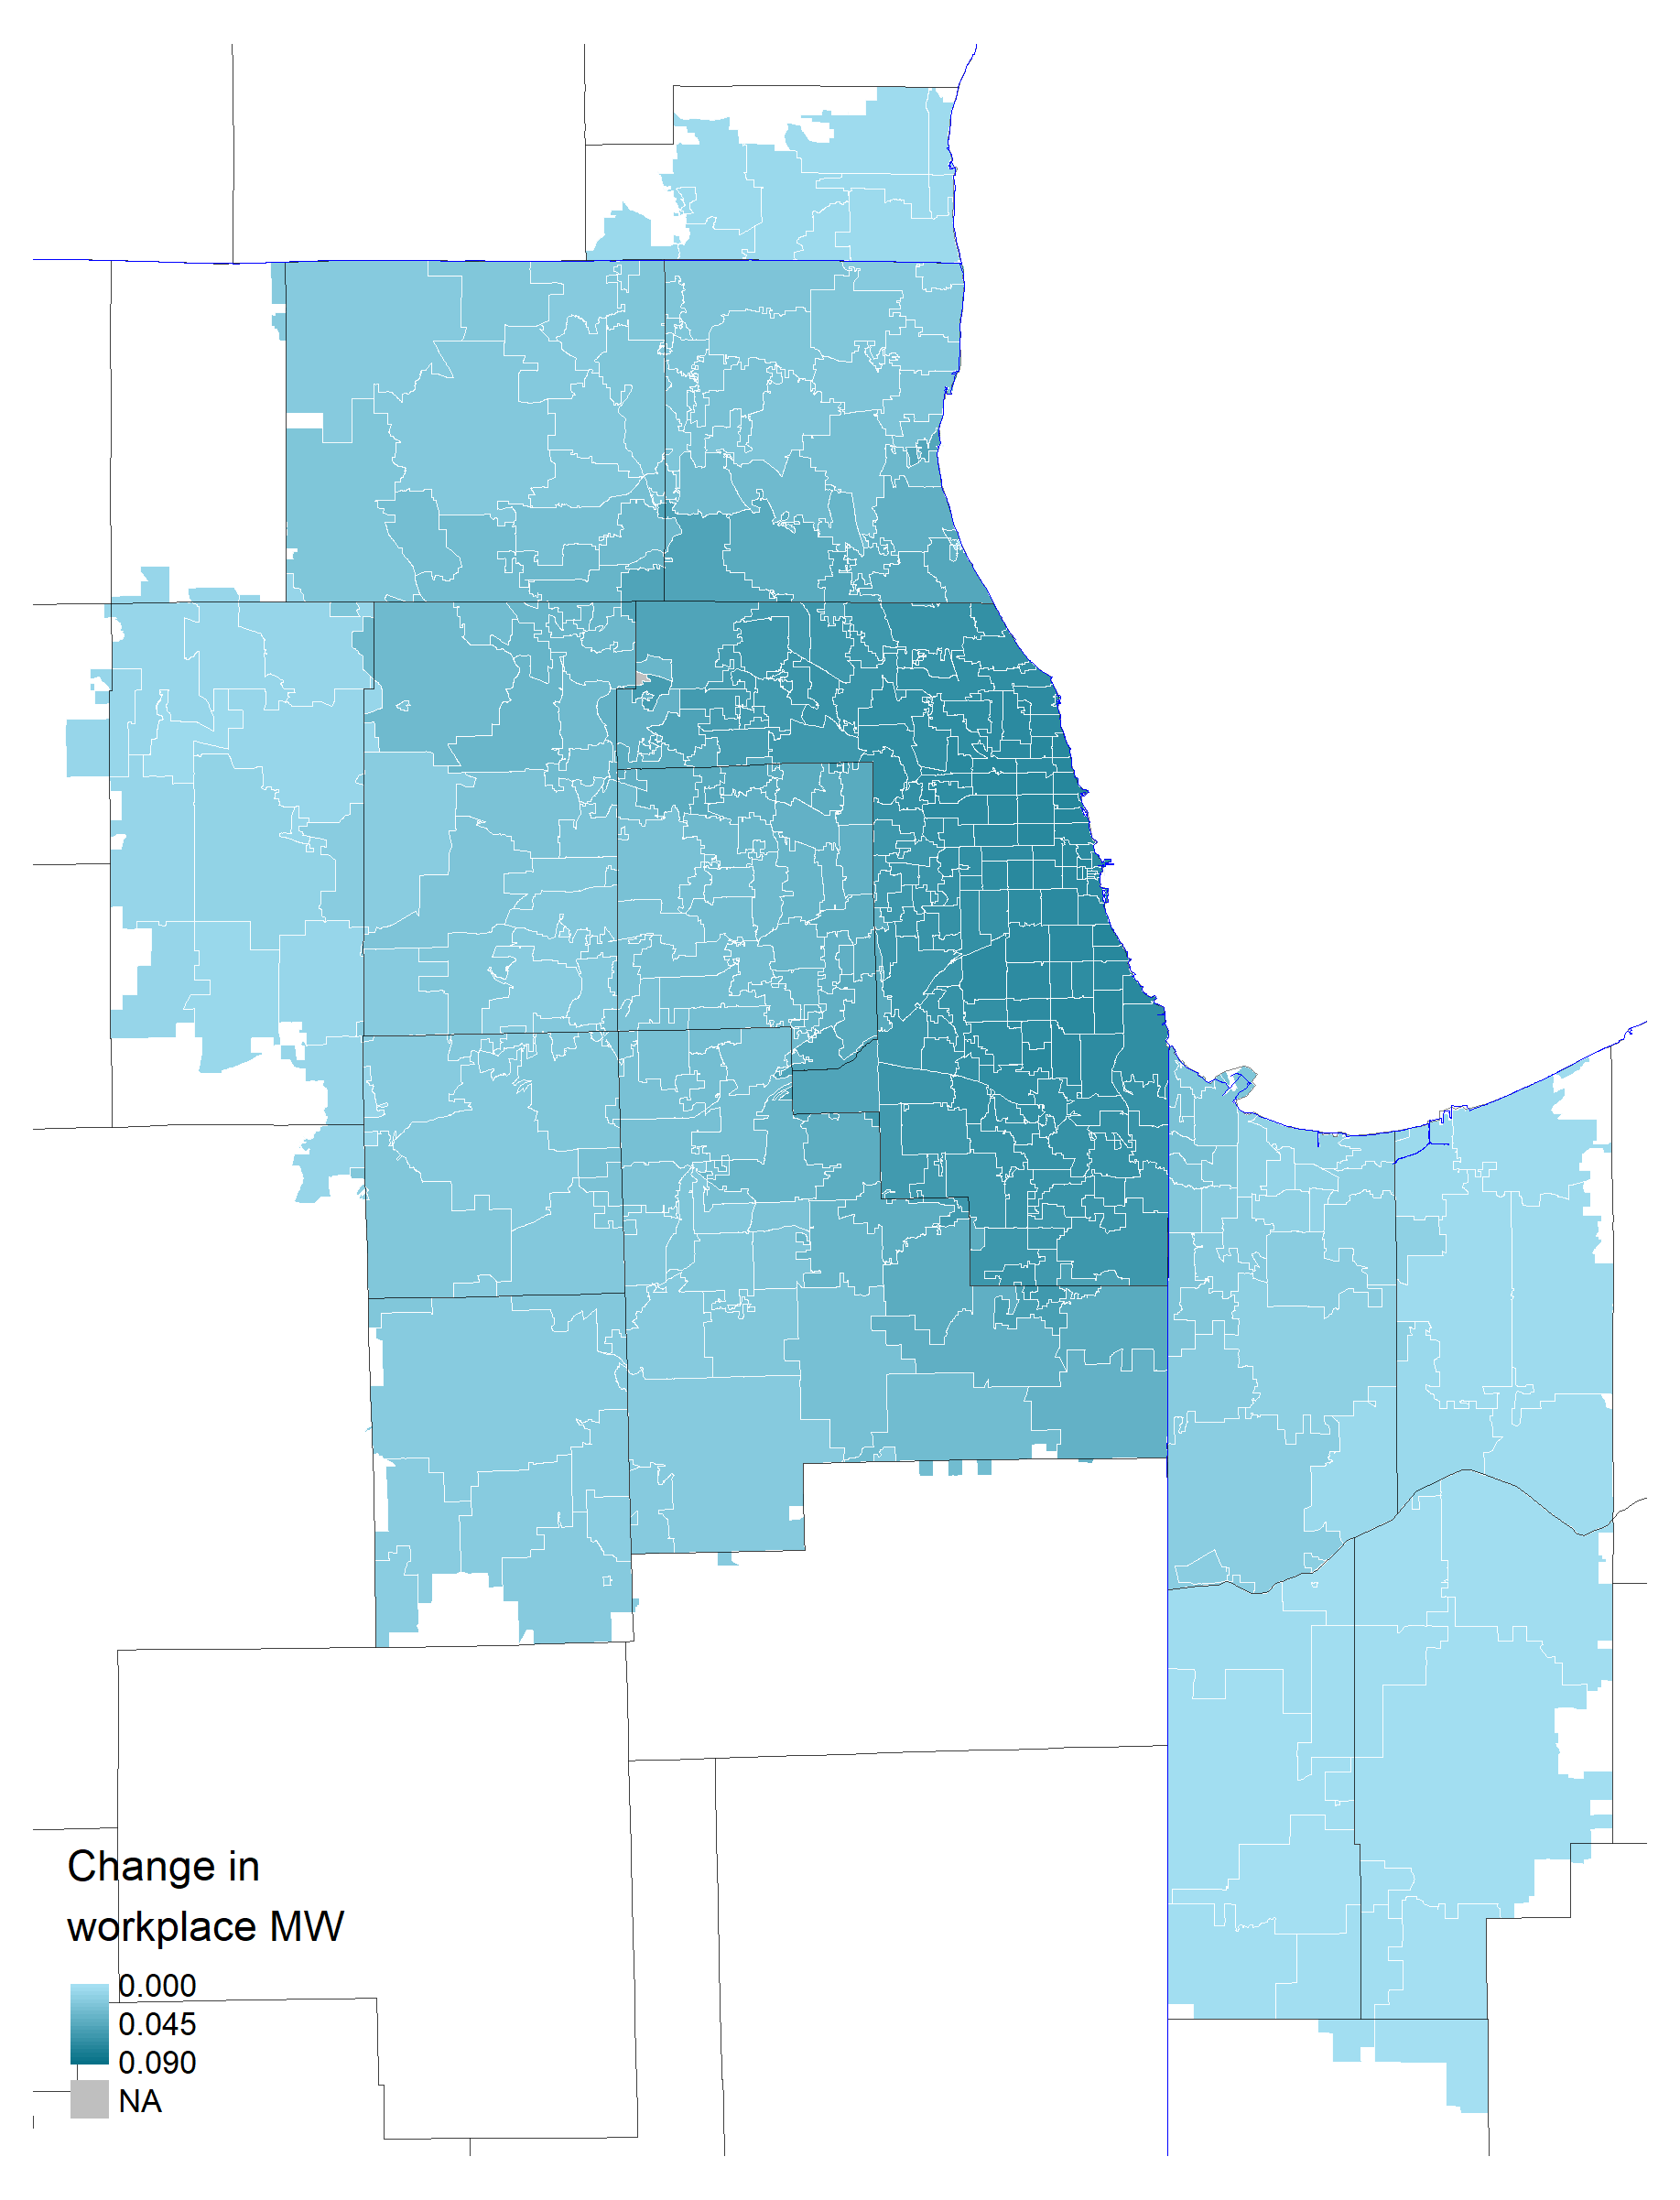
\includegraphics[width = 0.99\textwidth]{maps_events/output/chicago2019-6_wkp_mw.png}
            \caption*{Change in workplace MW}
        \end{subfigure}
        \begin{subfigure}{0.33\textwidth}
                         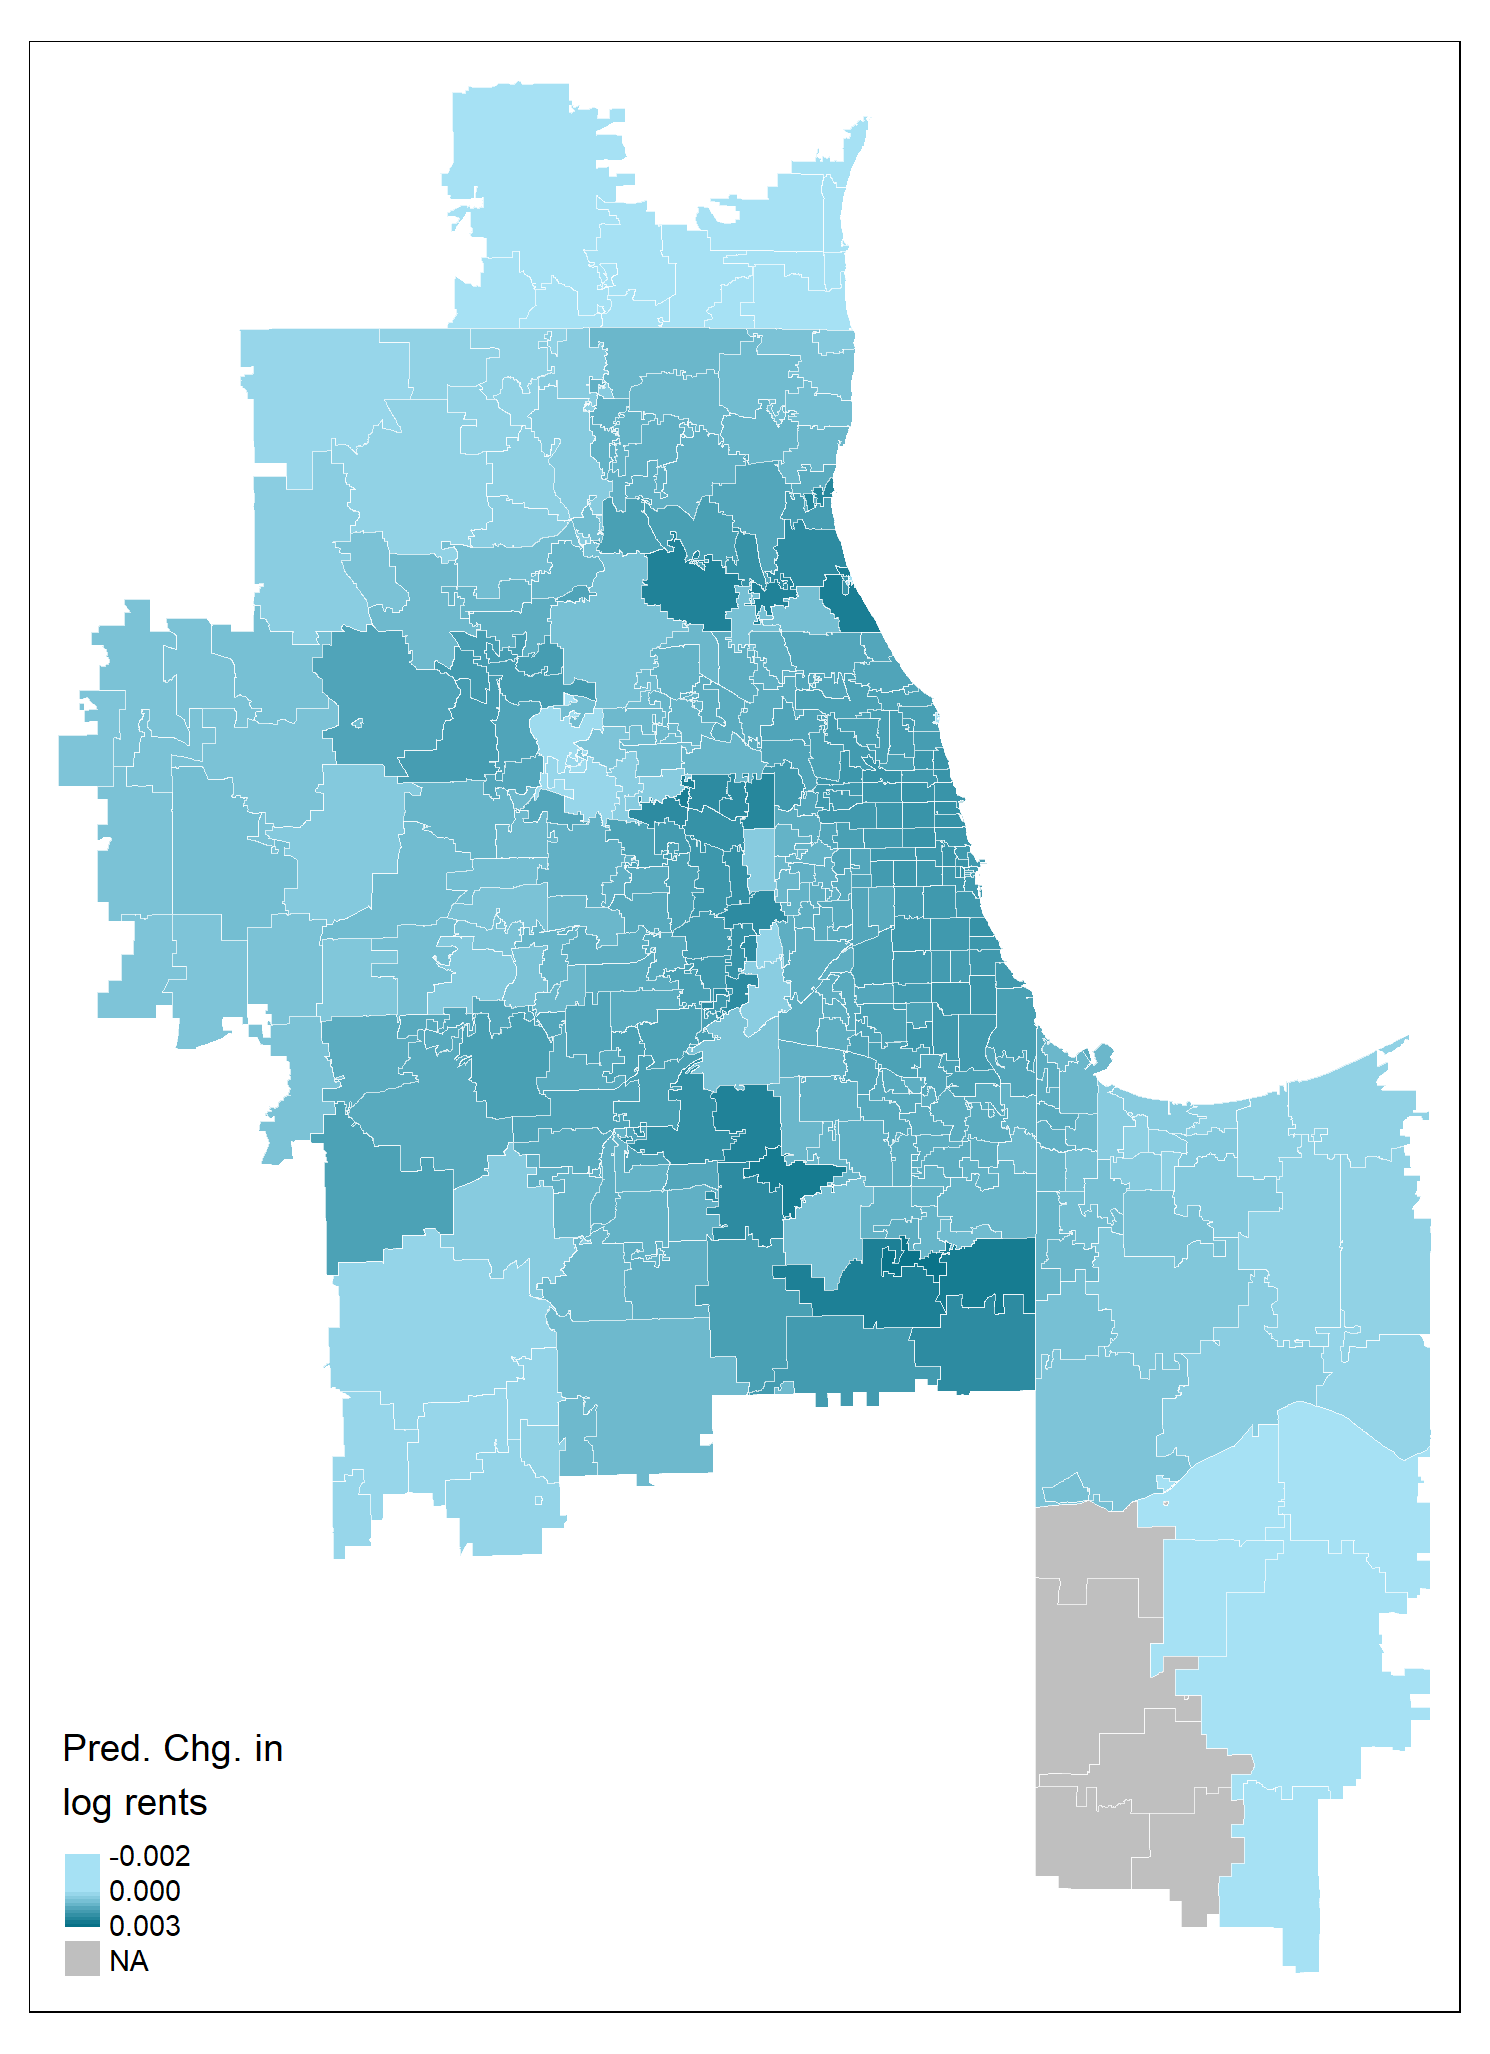
\includegraphics[width = 0.99\textwidth]{prediction_events/output/chicago_2019-7_hatfe_d_ln_rents_baseline.png}
            \caption*{Predicted change in log rents}
        \end{subfigure}
    \end{figure}
    
    \hyperlink{static_tab}{\beamerbutton{Go Back}}
\end{frame}


\end{document}